As stated in the previous chapter, IP multicast can be enabled in DMM by deploying the MLD proxy function at MAR. The multicast traffic is routed directly from the native multicast infrastructure via the current MAR for the new multicast flow. For the flow after handover, the multicast traffic is tunneled from the MAR where the flow is initiated to the current one via the mobility tunnel between them. Thus, the multicast mobility anchor (MMA) is assigned at the initial phase of the multicast flow (identical with the unicast mobility anchor): the MAR where the flow is initiated. The multicast flow will be anchored at the initially assigned MMA during its lifetime. Therefore, even when the MN moves far away from its anchor, the multicast traffic still traverses the anchor. As a result, it causes several issues to the ongoing multicast flow such as service disruption, non-optimal routing, end-to-end delay and packet duplication. These problems become serious when considering the interruption- and delay-sensitive services. Also, even the mobility anchors are distributed, some anchors are more overloaded than the others \cite{anchor_selection}.

In this chapter, we mainly argue the need for a dynamic multicast mobility anchor (DMMA) mechanism. From a service point of view, it helps satisfy the requirements in terms of service disruption and delay, especially when considering the real-time services. It provides a mechanism to better distribute the load among MARs. Moreover, other issues like packet duplication and leave latency (waste of resource) can be reduced. The DMMA takes into account not only the multicast service context (e.g., interruption-sensitive and delay-sensitive services) but also the mobile node's mobility context and the network context (such as current load of MARs and multicast channel policy), thus enabling a per-flow multicast support. In other words, each multicast flow can be treated differently upon different contexts. 

The rest of this chapter is organized as follows. Section \ref{c10:multicast_listener} introduces the issues and different approaches for the multicast listener support in a DMM environment. Section \ref{c10:quantitative_analysis} presents the performance analysis regarding different metrics as service disruption, end-to-end delay, signaling cost and packet loss. The DMMA mechanism is presented in Section \ref{c10:dmma}. Section \ref{c10:discussion} discusses the implementation work, the scenario in which the multicast router is deployed at MAR as well as the multicast source support. Finally, Section \ref{c10:conclusion} concludes this chapter and provides perspectives for future work. 

\section{Multicast Listener Mobility in DMM} \label{c10:multicast_listener}

This chapter follows the concept of the network-based DMM proposed by the IETF DMM Working Group\footnote{http://datatracker.ietf.org/wg/dmm/} as described in Chapter \ref{ch:reference_technologies}. We recall some abbreviations introduced in the previous chapters to denote the role of MAR from a mobile node point of view:
\begin{itemize}
\item Current MAR (cMAR) is the MAR to which the MN is currently attached.
\item Anchor MAR (aMAR) of an MN's address/session is the MAR where the prefix in use is allocated (and the session is initiated using this address as the source address).  
\item Previous MAR (pMAR) is the MAR where the MN was previously attached. 
\end{itemize}

As mentioned in Chapter \ref{ch:reference_technologies}, there is a limited work for the multicast support since the DMM is still in an early stage of standardization.  This chapter focuses on the scenario in which the MAR acts as an MLD proxy. Also, only multicast listener mobility in the network-based DMM is further studied. In this case, when a multicast flow is initiated, the multicast traffic is received directly from the native multicast infrastructure via the cMAR. After handover, the traffic is routed from the anchor to the current MAR via the tunnel between them (like unicast traffic). In this chapter, it is called the default multicast mode in DMM. However, this mode does not address any multicast-related issues caused by the movement of listener such as service disruption, packet loss, non-optimal routing, end-to-end delay, and tunnel convergence problem (for further information, see Chapter \ref{ch:reference_technologies}). 

Regarding the service disruption, when a multicast listener moves from the pMAR to the cMAR, it may cause a noticeable service disruption for the ongoing flows. As a result, the multicast context transfer is required to avoid a large delay caused by multicast-related procedures (about 5s in the normal case, and 2.5s in the best case) \cite{Thinh_WCNC_Multicast}. This delay is much longer than the maximum tolerant interruption time for normal services, as specified in \cite{interruption_requirements} is 500 ms. Even with the multicast context transfer, it is unable to meet the requirement in terms of service disruption for the interruption-sensitive service when the delay cMAR-aMAR is large \cite{Thinh_ICNS, multicast_DMM_Sergio_PIMRC}. It is because the multicast traffic has to pass through the aMAR, which plays the role of multicast mobility anchor (MMA).  

Also, since the multicast traffic always traverses the aMAR, it often results in a longer route (e.g., when the source and the listener are close to each other but far from the listener's aMAR). In particular, when considering a significant large domain, it can cause a high end-to-end delay. This issue becomes serious when the end-to-end delay sensitive service is considered. 

In case of mobility, the utilization of the mobility tunnel for the multicast flow may result in the tunnel convergence problem. It occurs when multiple instances of the same multicast traffic converge to an MAR, leading to the redundant traffic. The main reason is that multiple MLD proxy instances are installed at MAR with their upstream interfaces configured to different aMARs. Since the purpose of DMM is moving the mobility anchors from the core to the edge of the networks, the number of mobility anchors in a DMM domain will be much more than that in a PMIPv6 domain. As a consequence, the tunnel convergence problem is supposed to be much more severe than that in PMIPv6. As stated in the DMM requirements \cite{DMM_requirements}, the multicast solutions in DMM should take this issue into consideration. By using an extension to MLD proxy to support multiple upstream interfaces \cite{multiple_upstreams}, the tunnel convergence problem can be avoided. In this case, only one proxy instance will be installed at MAR with its upstream interfaces being configured towards different aMARs and its upstream MR. Accordingly, the MAR will receive only one instance of the multicast packet.
\begin{figure}[tb!] 
  \begin{center} 
    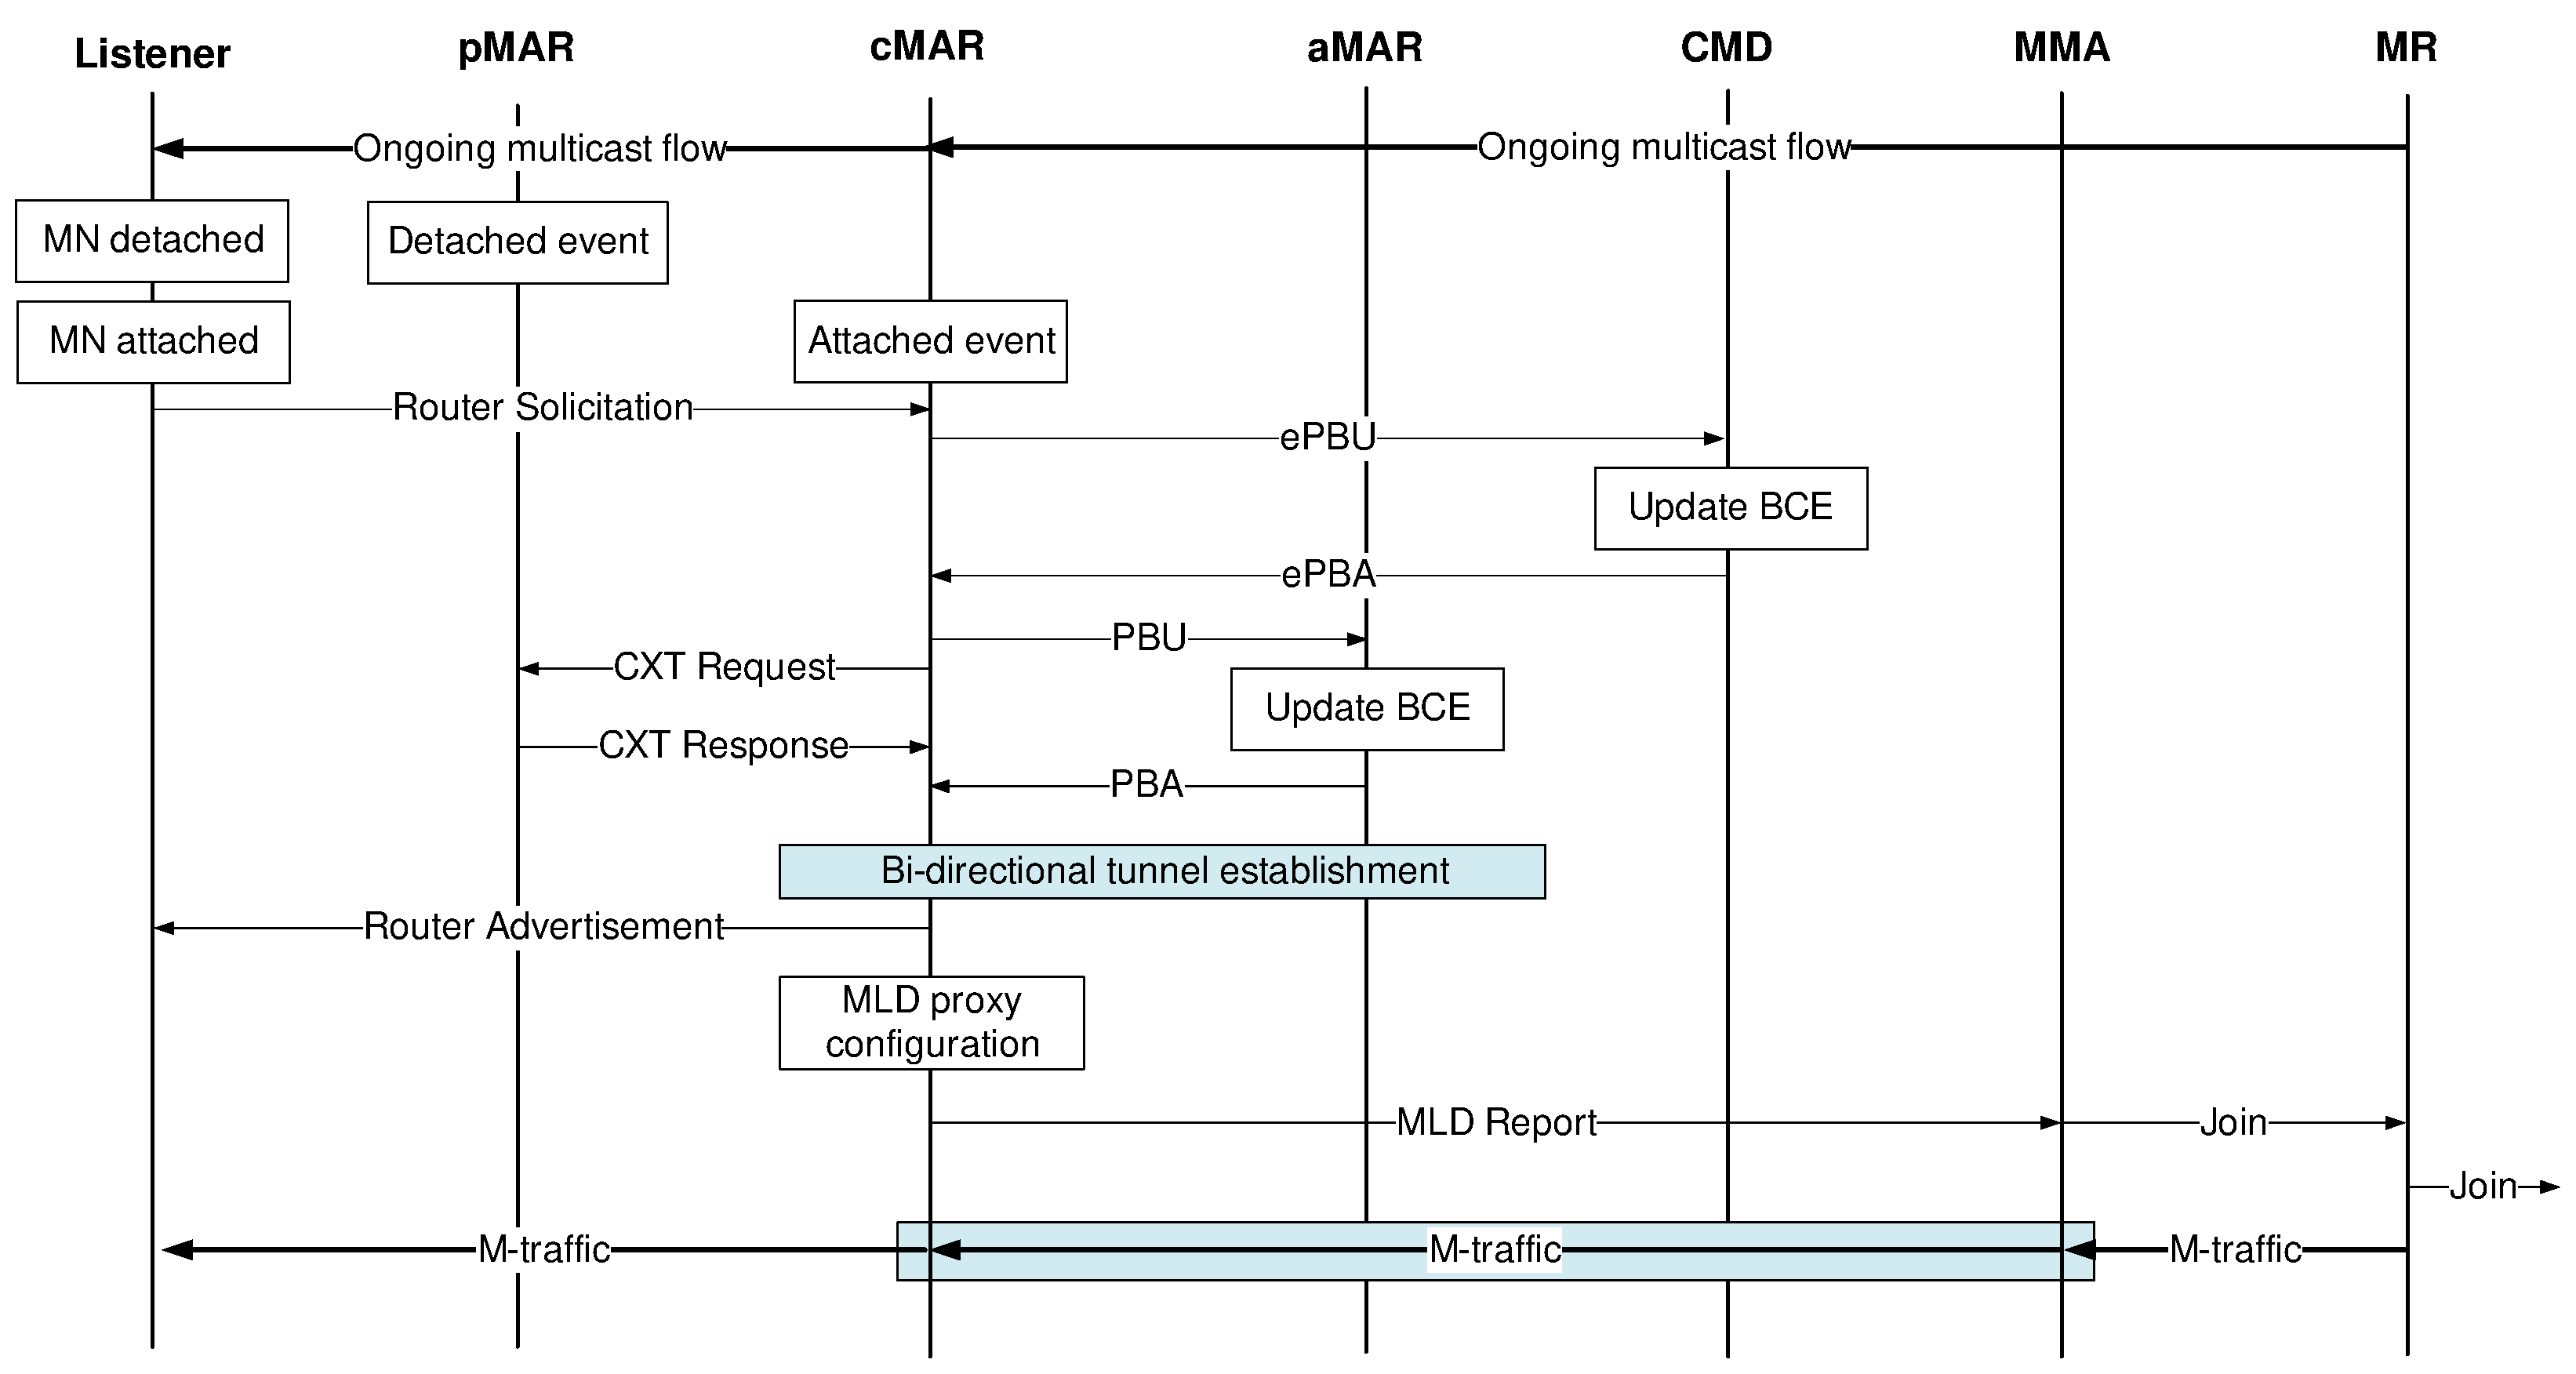
\includegraphics[width=0.90\textwidth]{./Part3/Chapter8/figures/c10_service_disruption_common.eps} 
    \caption[Signaling when a listener performs a handover in DMM.]{Signaling when a listener performs a handover in DMM.}
    \label{fig:c10_HO}
  \end{center} 
\end{figure}
To highlight these issues, this subsection considers different candidates for the MMA such as the aMAR (default mode), the pMAR, the cMAR (native subscription), or a common MMA (COMMA) which serves as only one MMA for the domain (as similar in \cite{direct_routing_mtma}). Different approaches MMA\_aMAR, MMA\_pMAR, MMA\_cMAR, and MMA\_COMMA are considered, accordingly. We also consider the impact of deploying MLD proxy with multiple upstream interfaces on the service disruption time, end-to-end delay and signaling cost. 

The signaling when a listener performs a handover in DMM is described in Fig.~\ref{fig:c10_HO}. The operations are briefly described as follows. The central mobility database (CMD), as an extended LMA, stores the MN's home network prefixes, its corresponding anchor points (aMAR) and its current location (cMAR). In case of handover, the cMAR allocates a new network prefix for this MN. The cMAR then sends a PBU to the CMD for the new prefix registration as well as retrieves the address of the anchoring MARs of the ongoing sessions. This message includes the MN\_ID, the allocated prefix at the current MAR. By looking up the BCE table, the CMD updates the entry corresponding to the MN\_ID with the current location of the MN. The CMD then replies by an extended PBA including the list of previous addresses and the corresponding prefixes. Upon receiving this message, the cMAR exchanges the PBU/PBA messages with the anchor MARs in order to update the current location of the MN. Thus, the bi-directional tunnel is established between the cMAR and each aMAR, if necessary. In parallel, the multicast context transfer messages are exchanged between the cMAR and the pMAR allowing the cMAR to obtain the active multicast subscription of the MN. For each flow, the cMAR configures an upstream interface towards the MMA (if necessary), and sends an MLD report to the MMA to join the flow. The MMA, after joining the multicast delivery tree, forwards the multicast packets to the cMAR via the tunnel between them. Finally, they reach the MN. 

\section{Quantitative Analysis} \label{c10:quantitative_analysis}
This section presents the quantitative analysis of different approaches regarding different metrics such as multicast service disruption, end-to-end delay, signaling cost and packet loss. 

\subsection{Network Model and Performance Metrics}
\subsubsection{Reference model}
\begin{figure}[tb!] 
  \begin{center} 
    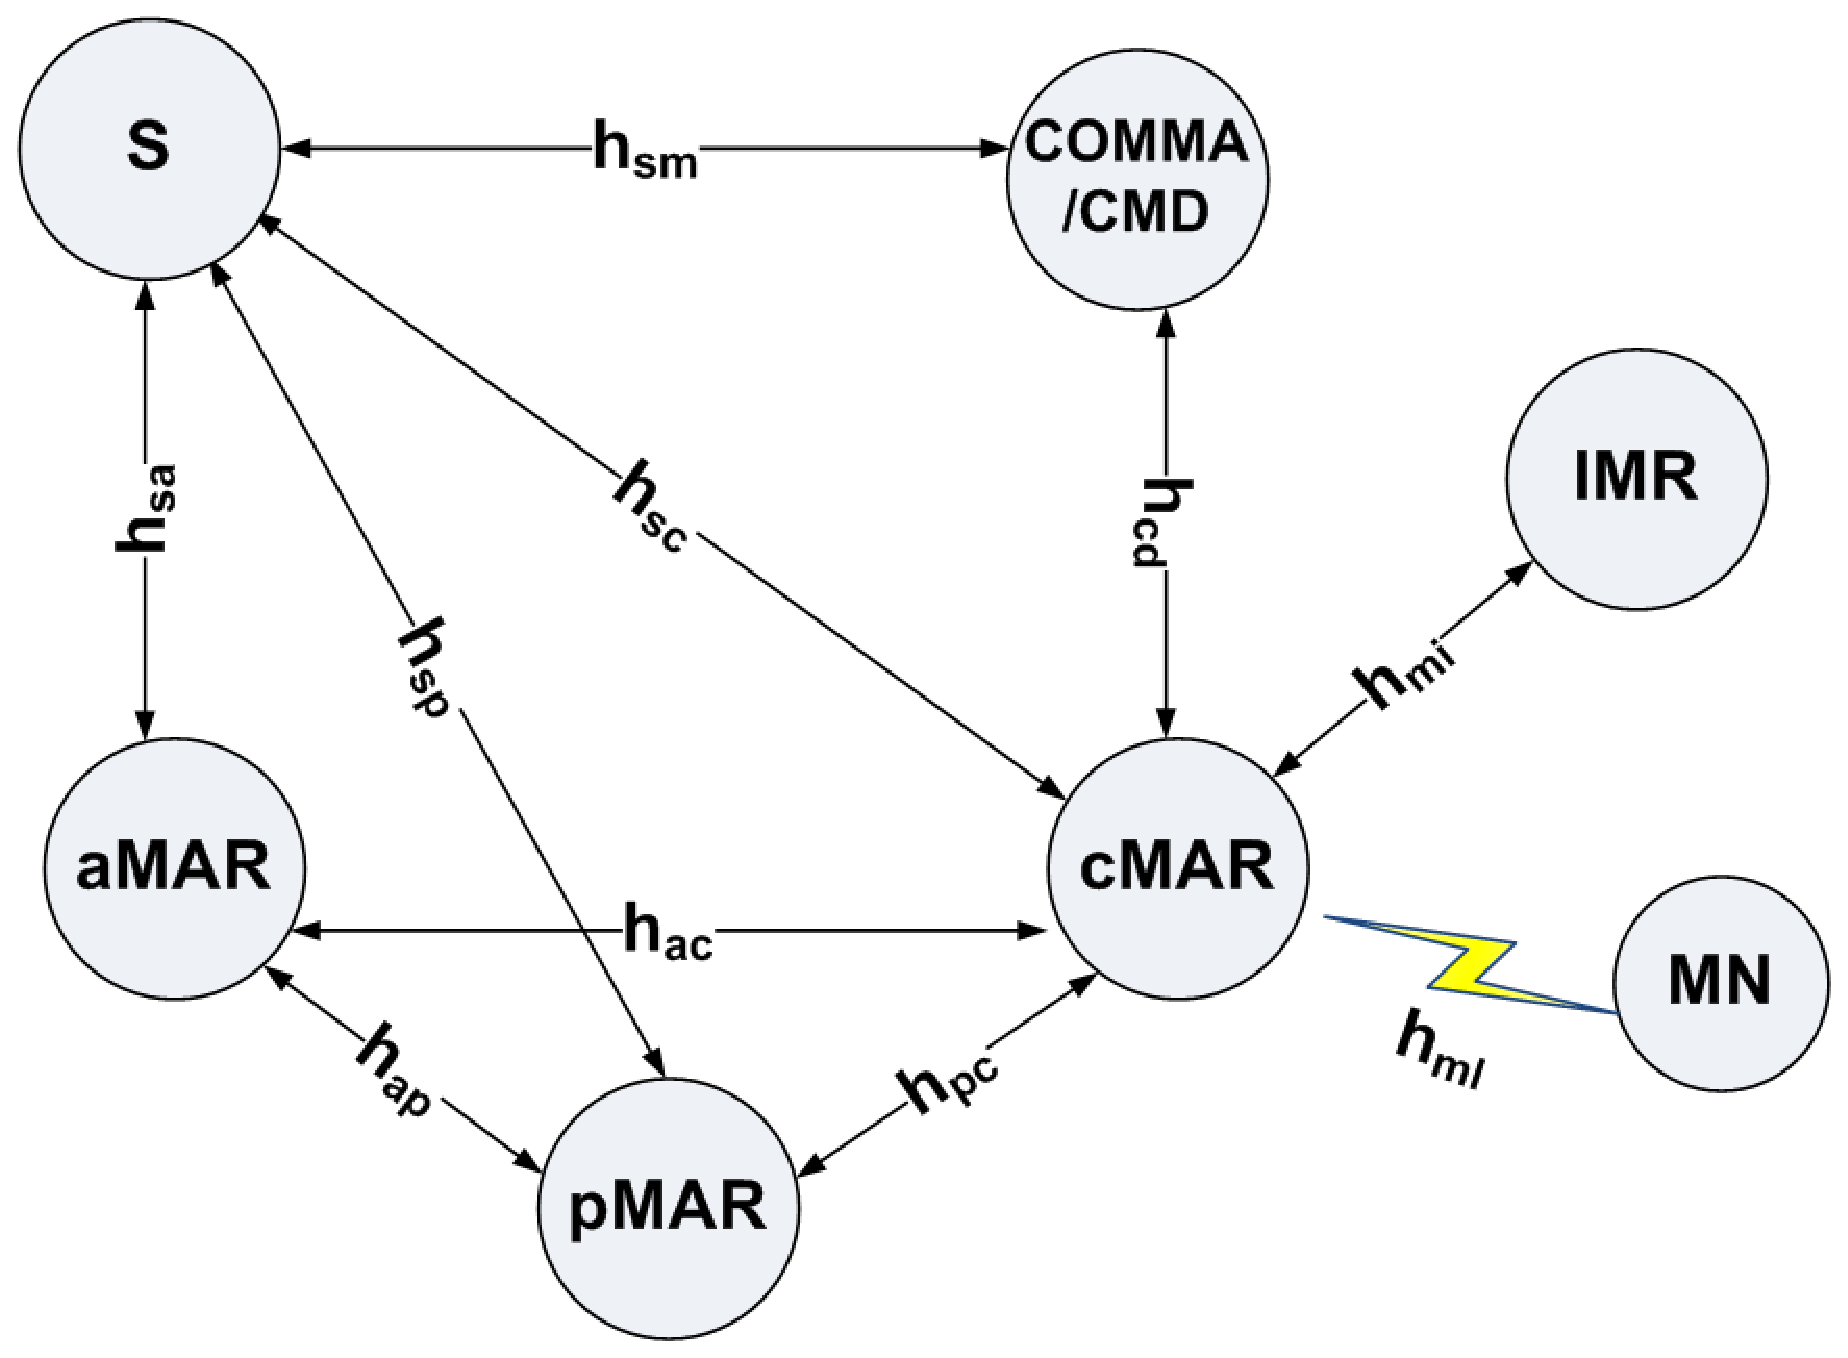
\includegraphics[width=0.55\textwidth]{./Part3/Chapter8/figures/c10_topology_analysis.eps} 
    \caption{Reference network topology.}
    \label{fig:c10_topology_analysis}
  \end{center} 
\end{figure}

Fig.~\ref{fig:c10_topology_analysis} shows a reference topology for the performance analysis. The hop-count distances between the entities are defined as follows:
\setlength \abovedisplayskip{-1pt}
\vspace{-0.1in}
\begin{itemize}
\itemsep 0.07em
\item $h_{ac}$: the average number of hops between the aMAR and the cMAR.
\item $h_{ap}$: the average number of hops between the aMAR and the pMAR.
\item $h_{pc}$: the average number of hops between the pMAR and the cMAR.
\item $h_{cd}$: the average number of hops between the MAR and the CMD/COMMA.
\item $h_{ml}$: the average number of hops between the MAR and the listener (MN), it is assumed to be one (wireless link).
\item $h_{sa}$: the average number of hops between the source S and the aMAR.
\item $h_{sp}$: the average number of hops between the source S and the pMAR.
\item $h_{sc}$: the average number of hops between the source S and the cMAR.
\item $h_{sm}$: the average number of hops between the source S and the COMMA.
\item $h_{mr}$: the average number of hops between the MAR and its upstream MR, it is assumed to be one. 
\item $h_{mi}$: the average number of hops between the cMAR and the intersection MR (IMR) which already has a multicast forwarding state for the group.
\end{itemize}

We then define the network scale $\psi$ which is the ratio between the number of hops between two adjacent MARs ($h_{mm}$) and the number of hops between the MAR and the CMD ($h_{cd}$).\\
\begin{equation}
\psi = \frac{h_{mm}}{h_{cd}}.
\end{equation} 
Typically, the average number of hops between two adjacent MARs is less than that between an MAR and a centralized entity. That means $\psi \leq 1$. In this chapter, we will investigate the impact of the network scale on the performance metrics by varying the value of $\psi$ over a range [0,1] (by varying $h_{mm}$ while fixing the value of $h_{cd}$). 
\subsubsection{Messages Related to the Performance Analysis}
As described in Fig.~\ref{fig:c10_HO}, various messages are used in our analysis. For a sake of simplicity, we suppose that there is only one ongoing flow. The following message sizes in bytes are considered in our analysis:
\begin{itemize}
\item $L_{RS}$: It is the size of the Router Solicitation (RS) message, which is 52.
\item $L_{RA}$: It is the size of the Router Advertisement (RA) message, which is 80.
\item $L_{PBU}$: It is the size of the PBU message, which is 84.
\item $L_{PBA}$: It is the size of the PBA message, which is 92.
\item $L_{ePBU}$: It is the size of the extended PBU message, which is 84.
\item $L_{ePBA}$: It is the size of the extended PBA message, which is 128.
\item $L_{M-Req}$: It is the size of the multicast context transfer request message, which is 86.
\item $L_{M-Res}$: It is the size of the multicast context transfer response message, which is 104.
\item $L_{C-Req}$: It is the size of the channel configuration request message, which is 92.
\item $L_{C-Res}$: It is the size of the channel configuration response message, which is 112. 
\item $L_{MLD-R}$: It is the size of the MLD Report message, which is 96.
\item $L_{Join}$: It is the size of the PIM Join message, which is 110.
\item $L_{MP}$: It is the size of the multicast packet, which is 200.
\item $L_{T}$: It is the size of the tunneling header, which 40.  
\end{itemize}

It is noted that the values of $L_{PBU}$,  $L_{PBA}$, $L_{ePBU}$, $L_{ePBA}$, $L_{M-Req}$ $L_{M-Res}$, $L_{C-Req}$ and $L_{C-Res}$ are taken from the real implementation of PMIPv6 \cite{oai_pmip} and the multicast context transfer function \cite{d4.4}, while the others are from \cite{HO_comparison_Lee,DMM_analysis_Hassan}.  

\subsubsection{Delay Model}
As described in Chapter \ref{ch:performance_evaluation}, we adopt the packet transmission delay model in \cite{packet_transmission_delay} in which the packet transmission consists of the transmission time and the propagation time.  
Thus, the transmission delay of a wired link can be calculated as\\
\begin{equation}
d_{wd}(l,h) = h (\dfrac{l}{BW_{wd}} + D_{wd}),
\end{equation}
where h is the hop-count distances between two nodes, l is the length of the packet, $BW_{wd}$ is the bandwidth of wired link and $D_{wd}$ is the wired link latency. 

Unlike the wired transmission which can be considered as reliable, the wireless link is unreliable. The wireless transmission delay is therefore calculated as \cite{packet_transmission_delay}\\
\begin{equation}
d_{wl}(l) = \dfrac{1}{1-q} (\dfrac{l}{BW_{wl}} + D_{wl}),
\end{equation} 
where q is the probability of wireless link failure, $BW_{wl}$ is the bandwidth of wireless link and $D_{wl}$ is the wireless link latency.  

\subsubsection{Mobility Model}
In this chapter, we consider the case where the MN always moves from MAR to MAR as if they were linearly deployed (the user is moving further away from the first attached MAR and never attaches back to a previously visited MAR). It represents the worst-case scenario. Thus, we have $h_{ac}$ = $h_{ap}$ + $h_{pc}$.
Let $N_{mar}$ denote the average number of MARs involved in the data traffic forwarding to/from an MN. In our context, $N_{mar}$ is also the number of handovers. We therefore obtain \\
\begin{equation}
h_{ac} = N_{mar} h_{mm},
\end{equation} 
\begin{equation}
h_{pc} = h_{mm}.
\end{equation}

In our analysis, the low value of $N_{mar}$ represents the low mobility node and the short-lived flow scenarios. The higher value of $N_{mar}$ corresponds to the high mobility and long-lived flow scenarios.   

\subsection{Analytical Modeling}
This subsection develops an analytical model regarding the following performance metrics: the multicast service disruption time ($SD(.)$), representing the period when the listener cannot receive the multicast packet; the end-to-end delay ($E2E(.)$) - the transmission time from source to listener; the signaling cost ($SC(.)$) - the cost for supporting multicast handover; the packet delivery cost ($DC(.)$) - the cost to deliver multicast packets from the source to the listener; the packet tunneling cost ($TC(.)$) - the tunnel overhead;  and packet loss ($\varphi_{p}$) - the number of lost packets during handover. In the performance analysis, we consider the normal case and the case where the MLD proxy supports the multiple upstream interfaces capability. We then highlight the impacts and benefits of using multiple upstream interfaces on these metrics. 

\subsubsection{Multicast Service Disruption Time Analysis}
The multicast service disruption time ($SD(.)$) is defined as a period when a multicast listener is unable to receive the multicast packets. 
Assuming that the delay associated with the processing of the messages in the network entities (e.g., time for PBU processing and updating binding cache in MAR) is included in the total value of each variable. Then the service disruption time is (see Fig.~\ref{fig:c10_HO}) \\
\small
\begin{equation}
SD(.) = T_{L2} + d_{wl}(L_{RS}) +T_{CMD} + max \{ T_{LU}, T_{CXT}\}  +max \{d_{wl}(L_{MP}), T_{M}{(.)} + d_{wl}(L_{MP})\},
\label{eq:sd}
\end{equation}
\normalsize
where $T_{L2}$ is the L2 handover duration, $T_{CMD}$ is the time needed to get the address of the anchor/previous MAR from the CMD, $T_{LU}$ is the location update time (at the aMAR), $T_{CXT}$ is the time for the context transfer messages exchanged, $T_{M} (.)$ is the time needed for the cMAR to join and get the first multicast packet after handovers. 

In Eq.~(\ref{eq:sd}), except $T_{M}{(.)}$, the other components are the same in different approaches, and given by\\
\begin{equation}
T_{CMD} = d_{wd}(L_{ePBU},h_{cd}) + d_{wd}(L_{ePBA},h_{cd}),
\end{equation}
\begin{equation}
T_{LU} = d_{wd}(L_{PBA}, h_{ac}) + d_{wd}(L_{PBU}, h_{ac}),
\end{equation}
\begin{equation}
T_{CXT} = d_{wd}(L_{M-Req},h_{pc}) +d_{wd}(L_{M-Res},h_{pc}).
\end{equation}

In (\ref{eq:sd}), $T_{M}^{(.)}$ represents the time needed for the cMAR to join and get the first multicast packet. In case of MMA\_cMAR, the cMAR has to get the multicast traffic from the IMR which already has a multicast forwarding state for this group. Thus, \\
\small
\[ T_{M}(cMAR) = \left\{ 
 \begin{array}{l l}
   \overline{w}_{mr} \quad \small \text{if } h_{mi} =0,  \\
   (h_{mi} +1) \overline{w}_{mr}+d_{wd}(L_{MLD-R}) + d_{wd}(L_{MP}) +  d_{wd}(L_{Join},h_{mi}-1) \\+d_{wd}(L_{MP},h_{mi}-1)   \quad \small \text{if }h_{mi} \geq 1. 
 \end{array} \right.\] 
\normalsize 
where $\overline{w}_{mr}$ is the delay time in which an MR (and an MLD proxy) needs to join a multicast flow at each router (proxy) in the internet \cite{MPDSR}. 

In case of MMA\_pMAR, the pMAR already had the multicast state for this flow. We have \\
\begin{equation}
T_{M}(pMAR) = 2\overline{w}_{mr} +d_{wd}(L_{MLD-R}+L_{T},h_{pc})+d_{wd}(L_{MP} +L_{T},h_{pc}).
\end{equation}

In case of MMA\_aMAR, there are two possibilities: the normal case (case 1, without deploying the multiple upstream interfaces, thus, corresponding to the default mode), and the case where MLD proxy with multiple upstream interfaces is deployed at MARs. In the latter case, in the worst situation, the aMAR needs to join the multicast channel, leading to an extra delay. It happens, for example, in case the multicast traffic was received from the multicast infrastructure in the pMAR and the aMAR has left the channel. Let $p_{a}$ denote the probability that this situation happens. As a result, $T_{M}(.)$ is calculated as \\
\begin{equation}
T_{M}(aMAR) =(1-p_{a}) T_{M}(aMAR-c1)  +p_{a} T_{M}(aMAR-wc),
\end{equation}
where
\begin{equation}
T_{M}(aMAR-c1) =2\overline{w}_{mr} +d_{wd}(L_{MLD-R}+L_{T},h_{ac})+d_{wd}(L_{MP} +L_{T},h_{ac}),
\end{equation}
\small
\[T_{M}(aMAR-wc)  = \left\{ 
 \begin{array}{l l}
   T_{M}(aMAR-c1)  \quad \small \text{if } h_{mi} =0,  \\
    T_{M}(aMAR-c1)+ d_{wd}(L_{MLD-R})+ d_{wd}(L_{MP})  + d_{wd}(L_{Join},h_{mi}-1) \\+ (h_{mi}+1)  \overline{w}_{mr} +d_{wd}(L_{MP},h_{mi}-1)  \quad \small \text{if }h_{mi} \geq 1. 
 \end{array} \right.\] 
\normalsize 

It is noted that $T_{M}(aMAR-c1)$ represents the multicast service disruption time in the default mode, when $T_{M}(aMAR)$ shows the impact of using MLD proxy with multiple upstream interfaces on the service disruption time. As a result, $SD(aMAR)$ can be considered as a trade-off between the service disruption and the tunnel convergence problem.  

In case of MMA\_COMMA, we have \\
\begin{equation}
T_{M}(COMMA)= 2\overline{w}_{mr}+  d_{wd}(L_{MLD-R}+L_{T}, h_{cd}) + d_{wd}(L_{MP}+L_{T}, h_{cd}).
\end{equation}
\subsubsection{End-to-End Delay}
End-to-end delay ($E2E(.)$) is the packet transmission delay from the source to the listener. In the MMA\_cMAR, the cMAR receives the multicast traffic directly from the multicast infrastructure. Hence, the end-to-end delay is given by\\
\begin{equation}
E2E(cMAR) = d_{wd}(L_{MP},h_{sc}) + d_{wl}(L_{MP}).
\end{equation}

In the MMA\_aMAR, the multicast packet is routed from the source to the cMAR via the aMAR, representing the default multicast mode. We have \\
\begin{equation}
E2E(aMAR) = d_{wd}(L_{MP},h_{sa}) + d_{wd}(L_{MP}+L_{T},h_{ac}) + d_{wl}(L_{MP}).
\end{equation}

In case of MMA\_pMAR, the MAR always receives the multicast traffic from its pMAR in the normal case. Therefore, the end-to-end delay is given as follows \\
\begin{equation}
E2E(pMAR-c1)= d_{wd}(L_{MP},h_{sa}) + d_{wd}(L_{MP} +L_{T},h_{ap}) + d_{wd}(L_{MP} + L_{T},h_{pc})  + d_{wl}(L_{MP}).
\end{equation}

In case of using multiple upstream interfaces, we suppose that $p_{p}$ is the probability that the MAR gets multicast traffic from its upstream interfaces. Thus, $1-p_{p}$ is the probability the MAR gets the multicast traffic from its pMAR. The end-to-end delay in case of MMA\_pMAR is therefore given by
\begin{multline}
E2E(pMAR)=   d_{wl}(L_{MP}) + [d_{wd}(L_{MP},h_{sa})+ N_{mar} d_{wd}(L_{MP} +L_{T},h_{mm})] p_{p}^{N_{mar}-1} \\+ \sum_{i=1}^{N_{mar}-1} [d_{wd}(L_{MP},h_{i})+ (N_{mar}-i) d_{wd}(L_{MP} +L_{T},h_{mm})] p_{p}^{N_{mar}-i-1} (1-p_{p}),
\end{multline}
where $h_{i}$ is the hop-count distances from the source to the $i^{th}$ MAR in the moving path of the MN (from the aMAR to the cMAR), for example, $ h_{N_{mar}-1} = h_{sp}$ .  

Considering the MMA\_COMMA, the end-to-end delay is expressed as\\
\begin{equation}
E2E(COMMA) = d_{wd}(L_{MP},h_{sm})  + d_{wd}(L_{MP}+L_{T},h_{cd}) + d_{wl}(L_{MP}).
\end{equation}

\subsubsection{Cost Analysis}
In this subsection, the signaling cost ($SC(.)$), the packet delivery cost ($PC(.)$) and the tunneling cost ($TC(.)$) are investigated. The signaling cost (per handover) is the signaling overhead for supporting the handover including multicast-related procedures. It can be calculated as \\
\begin{equation}
SC(.) =SC_{LU} + SC_{M}(.),
\end{equation}
where $SC_{LU}$, $SC_{M}(.)$ is the signaling cost for the location update and the multicast-related procedures, respectively. As mentioned in Chapter \ref{ch:performance_evaluation}, the signaling message delivery cost is calculated as the product of the message size, the hop distance and the unit transmission cost in a wired/wireless link ($\alpha$ for the wired and $\beta$ for the wireless link). $SC_{LU}$ is therefore given by\\
\begin{equation}
SC_{LU} = \beta (L_{RS} + L_{RA}) + \alpha (L_{ePBU}  h_{cd} + L_{ePBA} h_{cd})  + \alpha (L_{PBU}  h_{ac} + L_{PBA} h_{ac}).
\end{equation}
$SC_{M}(.)$ is expressed as\\
\begin{equation}
SC_{M}(cMAR) = \alpha  (L_{M-Req}  h_{pc} + L_{M-Res} h_{pc} + L_{MLD-R} + L_{Join} h_{mi}).
\end{equation}
\begin{equation}
SC_{M}(pMAR) = \alpha (L_{M-Req}  h_{pc} + L_{M-Res} h_{pc} + L_{MLD-R} h_{pc}).
\end{equation}
\begin{equation}
SC_{M}(aMAR) =(1-p_{a}) SC_{M}(aMAR-c1)  + p_{a} SC_{M}(aMAR-wc),
\end{equation}
where 
\begin{equation}
SC_{M}(aMAR-c1) = \alpha (L_{M-Req}  h_{pc} + L_{M-Res} h_{pc} +L_{MLD-R} h_{ac}),
\end{equation}
\begin{equation}
SC_{M}(aMAR-wc) = \alpha (L_{M-Req}  h_{pc} + L_{M-Res} h_{pc}  + L_{MLD-R} h_{ac}+L_{MRD-R} +L_{Join} h_{mi}).
\end{equation}

\begin{equation}
SC_{M}(COMMA) = \alpha (L_{M-Req}  h_{pc} + L_{M-Res} h_{pc}  + L_{MLD-R} h_{cd}).
\end{equation}

The packet delivery cost represents the cost of delivering multicast packets to the MN per unit of time. Let $S_{c}$, $\lambda_{p}$ denote the average session length at the cMAR and the packet arrival rate, respectively. Again, the packet delivery cost in the MMA\_aMAR corresponds to the default multicast mode. The packet delivery cost is expressed as\\
\begin{equation}
PC(cMAR) = S_{c} \lambda_{p} (\alpha L_{MP} h_{sc}  + \beta L_{MP}).
\end{equation}
\begin{equation}
PC(aMAR) = S_{c} \lambda_{p} [\alpha L_{MP} h_{sa} + \alpha (L_{MP} + L_{T}) h_{ac}  + \beta L_{MP}].
\end{equation}

In case of MMA\_pMAR, in the normal case, the MAR always receives the multicast traffic from its pMAR. Thus, the packet delivery cost is given as follows \\
\begin{equation}
PC(pMAR-c1)=  S_{c} \lambda_{p} [\alpha  L_{MP} h_{sa} +  \alpha  (L_{MP} + L_{T}) ( h_{ap} + h_{pc}) + \beta L_{MP}].
\end{equation}
Using the multiple upstream interfaces, the packet delivery cost is calculated as
\begin{multline}
PC(pMAR)= S_{c} \lambda_{p}  \beta L_{MP} +  S_{c} \lambda_{p} [\alpha L_{MP} h_{sa}+ \alpha N_{mar}  (L_{MP} +L_{T}) h_{mm}] p_{p}^{N_{mar}-1} \\+ S_{c} \lambda_{p} \sum_{i=1}^{N_{mar}-1} [\alpha L_{MP} h_{i}+ \alpha  (N_{mar}-i) (L_{MP} +L_{T}) h_{mm}] p_{p}^{N_{mar}-i-1} (1-p_{p}).
\end{multline}

In case of MMA\_COMMA, the packet delivery cost is\\
\begin{equation}
PC(COMMA) = S_{c} \lambda_{p} [\alpha L_{MP} h_{sm} + \alpha (L_{MP} + L_{T}) h_{cd}  + \beta L_{MP}].
\end{equation}

Regarding the packet tunneling cost, it is defined as the additional cost from the tunneling overhead. In MMA\_cMAR, the multicast traffic is received directly from the multicast infrastructure, thus, there is no tunneling cost. On the contrary, in MMA\_aMAR, MMA\_pMAR, and MMA\_COMMA the traffic is routed via the tunnel aMAR-cMAR, pMAR-cMAR, and cMAR-COMMA, respectively. Note that the tunneling cost in the MMA\_aMAR corresponds to the default multicast mode. The tunneling cost is therefore computed as\\ 
\begin{equation}
TC(cMAR) = 0. 
\end{equation}
\begin{equation}
TC(aMAR) = \alpha  S_{c} \lambda_{p} (L_{MP} + L_{T}) h_{ac}. 
\end{equation}
\begin{equation}
TC(pMAR)=  \alpha  S_{c} \lambda_{p} (L_{MP} + L_{T}) h_{mm}  \sum_{i=0}^{N_{mar-1}} (N_{mar}-i)p_{p}^{N_{mar}-i-1} (1-\theta p_{p}).
\end{equation}
where 
\[\theta  = \left\{ 
 \begin{array}{l l}
   0 \quad \small \text{if } i =0,  \\
    1  \quad \small \text{if } i \geq 1. 
 \end{array} \right.\] 

\begin{equation}
TC(COMMA) = \alpha  S_{c} \lambda_{p} (L_{MP} + L_{T}) h_{cd}. 
\end{equation}

The signaling cost in general is an important factor which influences the scalability of the networks. However, as data and control plane are no longer coupled, in case where a huge amount of traffic is generated in the network, the packet delivery cost and tunneling cost play more important role.  
 
\subsubsection{Packet Loss}
During the handover, packets may be lost. The number of lost packets is proportional to the service disruption time and the packet arrival rate. As a result, the number of lost packets is given by\\
\begin{equation}
\varphi_{p}(.)= \lambda_{p} SD(.).
\end{equation}

\normalsize
\subsection{Numerical Results}
This subsection presents the numerical results based on the analysis given in the previous one. The default parameter values for the analysis are introduced in Table \ref{tap:c10_parameters}, in which some parameters are taken from \cite{dsrm}\cite{d4.4}. It is worth noting that the $SD (aMAR-c1)$, $E2E(aMAR)$, $SC(aMAR-c1)$, $PC(aMAR)$, and $TC(aMAR)$ correspond to the default mode in our analysis. \\

\begin{table}[ht]
\small
\caption{Parameters for the performance analysis.}
\label{tap:c10_parameters}
\centering
\begin{tabular}{|c |c |c |c |c |c |}
\hline
\textbf{Parameter} & \textbf{Value} & \textbf{Parameter} & \textbf{Value} & \textbf{Parameter} & \textbf{Value}  \\
\hline
$T_{L2}$ & 50ms & $BW_{wd}$  &  100Mbps & $BW_{wl}$  & 11 Mbps\\
\hline
  $D_{wd}$& 2ms  & $D_{wl}$ & 10ms & $q$& 0.35  \\
\hline
$\overline{w}_{mr}$&  10 ms  & $h_{mm}$ & 3 hops & $h_{cd}$&  12 hops  \\
\hline
$h_{mi}$& 2 hops  & $h_{sa}$& 16 hops  & $h_{sp}$&  16 hops   \\
\hline
 $h_{sc}$  & 16 hops   & $h_{sm}$&  16 hops &$S_{c} $&  60 s  \\
\hline
$\lambda_{p}$& 10 packets/s  & $\alpha$&  1 & $\beta $&  5  \\
\hline
$p_{p}$& 0.9  & $p_{a}$&  0.5 & & \\
\hline
\end{tabular}
\end{table}
\normalsize

\subsubsection{Multicast Service Disruption Time}
\begin{figure}[!h]
\centering
\subfloat[]{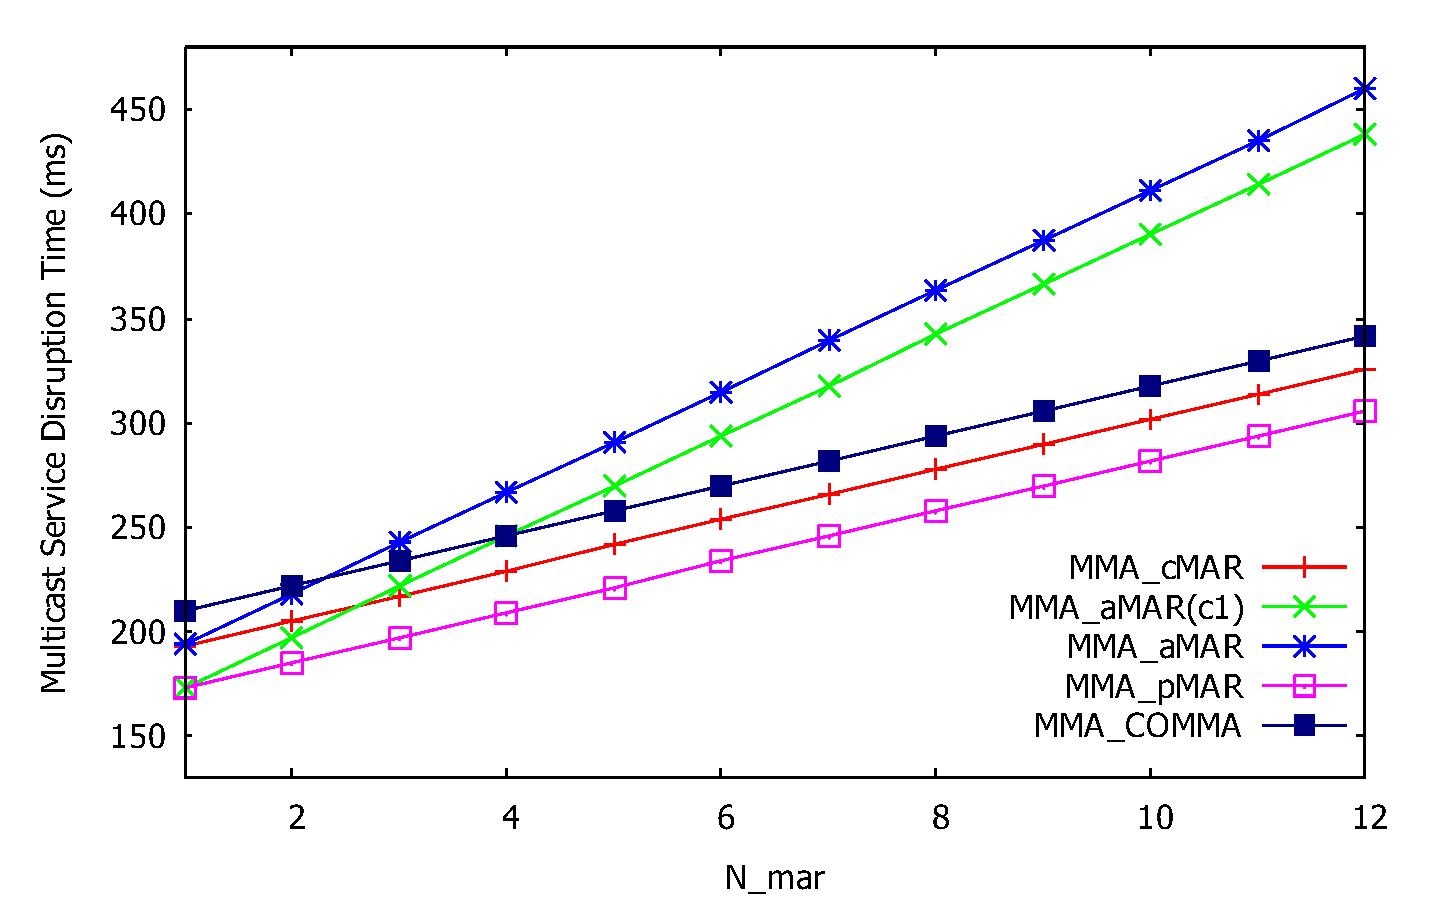
\includegraphics[scale=0.28]{./Part3/Chapter8/figures/c10_sd_n_mar.eps} \label{fig:c10_sd_n_mar}}
\subfloat[]{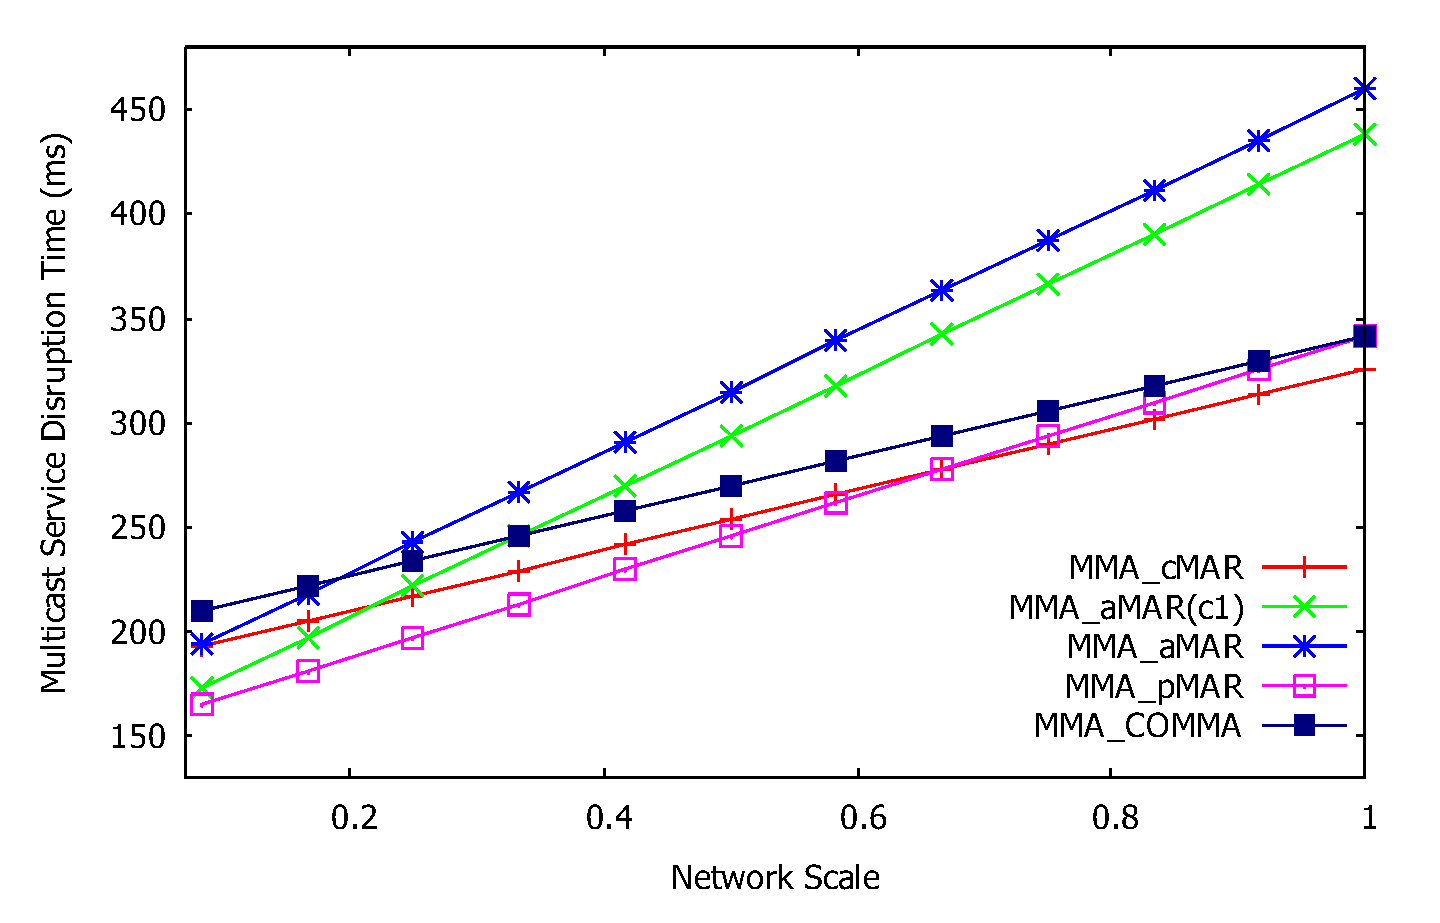
\includegraphics[scale=0.28]{./Part3/Chapter8/figures/c10_scale.eps}\label{fig:c10_scale}}\,
\subfloat[]{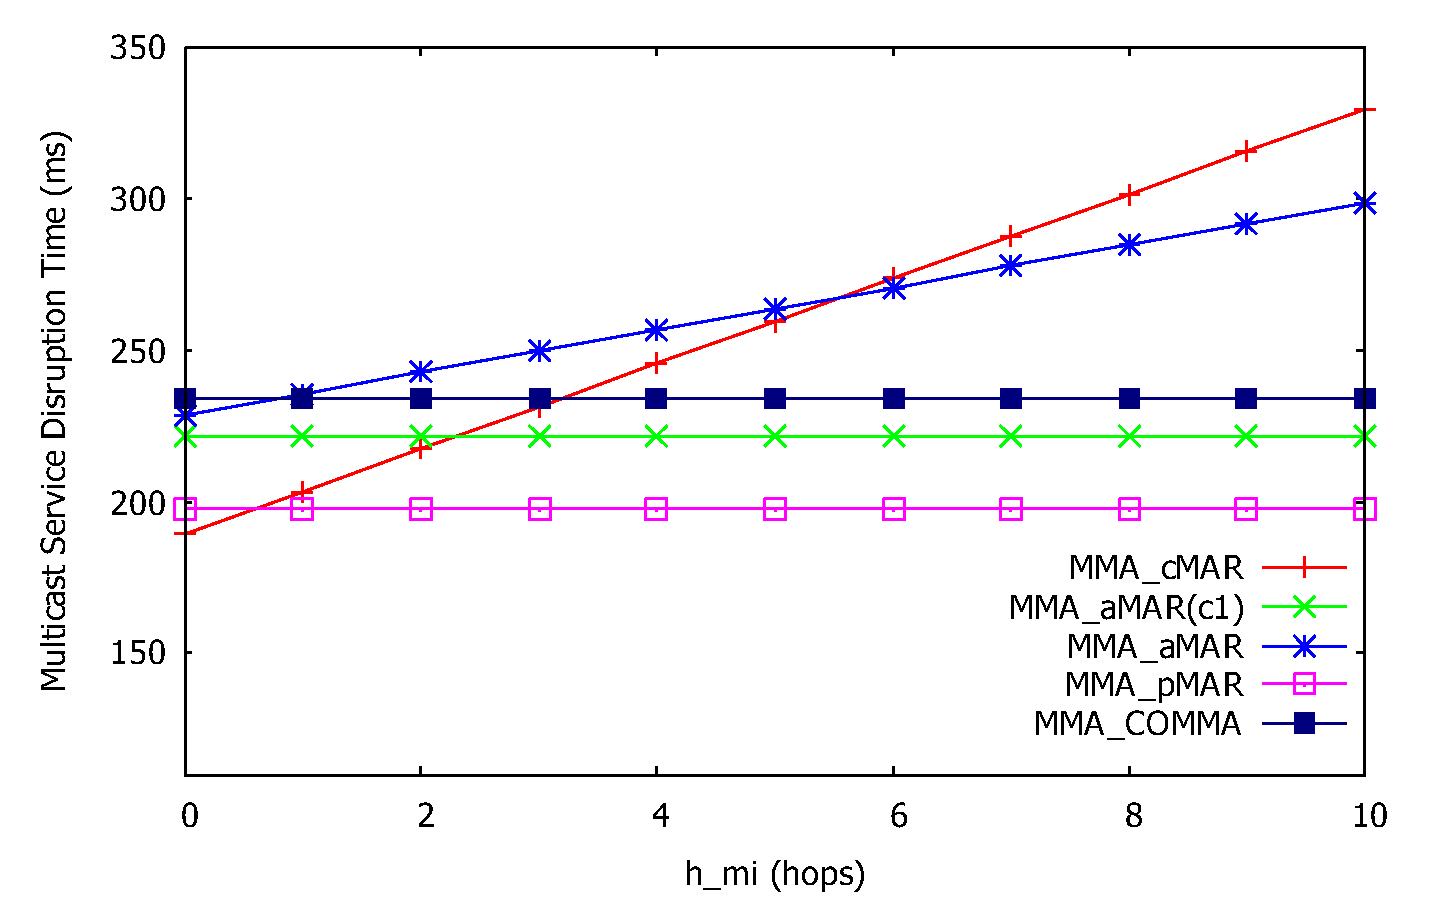
\includegraphics[scale=0.28]{./Part3/Chapter8/figures/c10_h_mi.eps}\label{fig:c10_h_mi}}
\caption[Multicast service disruption time.]{Multicast service disruption time as a function of: (a) $N_{mar}$, (b) $\psi$, (c) $h_{mi}$.}
\label{fig:c10_sd}
\end{figure}

Fig.~\ref{fig:c10_sd_n_mar} shows the multicast service disruption time when $N_{mar}$ is varied over a range from 1 to 12. It appears clearly that the MMA\_pMAR approach gives a better performance than the others (lower is better). The service disruption time in the MMA\_cMAR is slightly greater than that in the MMA\_pMAR since the value of $h_{mi}$ in this case is quite small (2 hops). When $N_{mar}$ is small (less than 5), all approaches satisfy the requirement in terms of service disruption for real-time services (lower than 300ms). When $N_{mar}$ is relatively big, the service disruption in case of MMA\_aMAR is significantly increased. We also investigate the impact of the network scale ($\psi$) on the service disruption time. In this case, $N_{mar}$ is set to a value of 3. In general, the impact of $\psi$ is similar to that of $N_{mar}$. Especially, Fig. \ref{fig:c10_scale} shows that there is an area where the MMA\_cMAR outperforms the MMA\_pMAR (when the network scale is larger than 0.62).

Fig.~\ref{fig:c10_h_mi} shows the multicast service disruption time when $h_{mi}$ is varied over a range from 0 to 10 hops. A small value of $h_{mi}$ indicates a high listener density scenario while a high value of $h_{mi}$ represents a low listener density scenario. The service disruption in the MMA\_pMAR is lower than that in the others (except when $h_{mi}=0$ indicating the case where the multicast traffic is already available at the cMAR's upstream MR). As the value of $h_{mi}$ increases, the service disruption time in the MMA\_pMAR, MMA\_aMAR (c1) and MMA\_COMMA is kept constant while that in the other cases is significantly increased. As a result, the difference between the approaches is increased. It comes from the fact that the multicast traffic is already available at the pMAR, aMAR, and COMMA in case of MMA\_pMAR, MMA\_aMAR(c1) and MMA\_COMMA, respectively. Additionally, the service disruption time in the MMA\_cMAR strongly depends on the value of $h_{mi}$. In other words, it cannot be guaranteed in the MMA\_cMAR approach. Also, in the MMA\_aMAR, it increases significantly compared to that in the MMA\_aMAR (c1) as a consequence of using multiple upstream interfaces in DMM. 

\begin{figure}[h!]
\centering
\subfloat[]{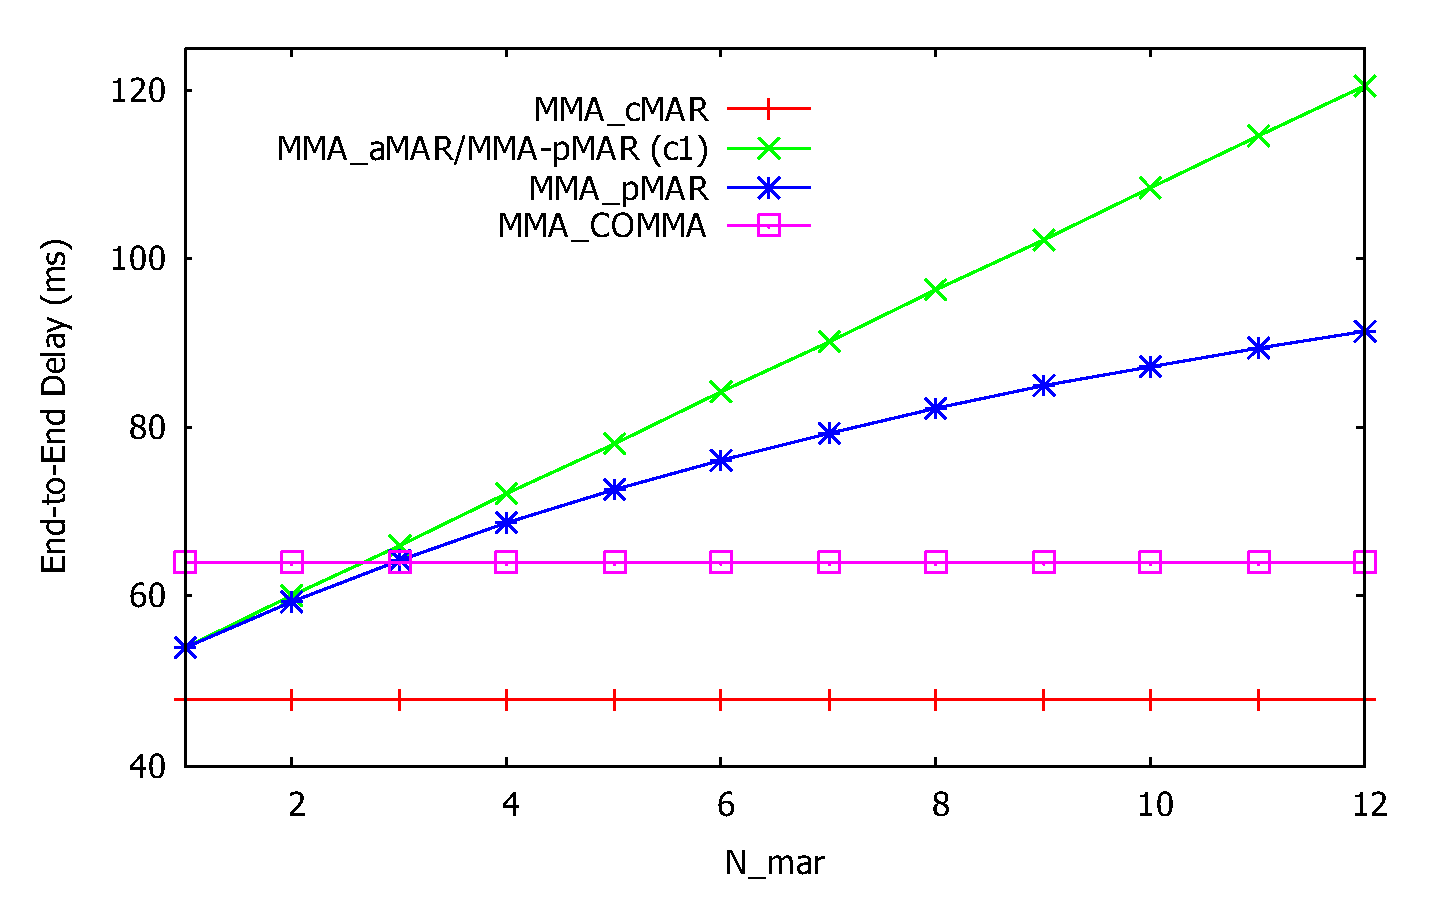
\includegraphics[width=0.50\textwidth]{./Part3/Chapter8/figures/c10_e2e_n_mar.eps} \label{fig:c10_e2e_n_mar}}
\subfloat[]{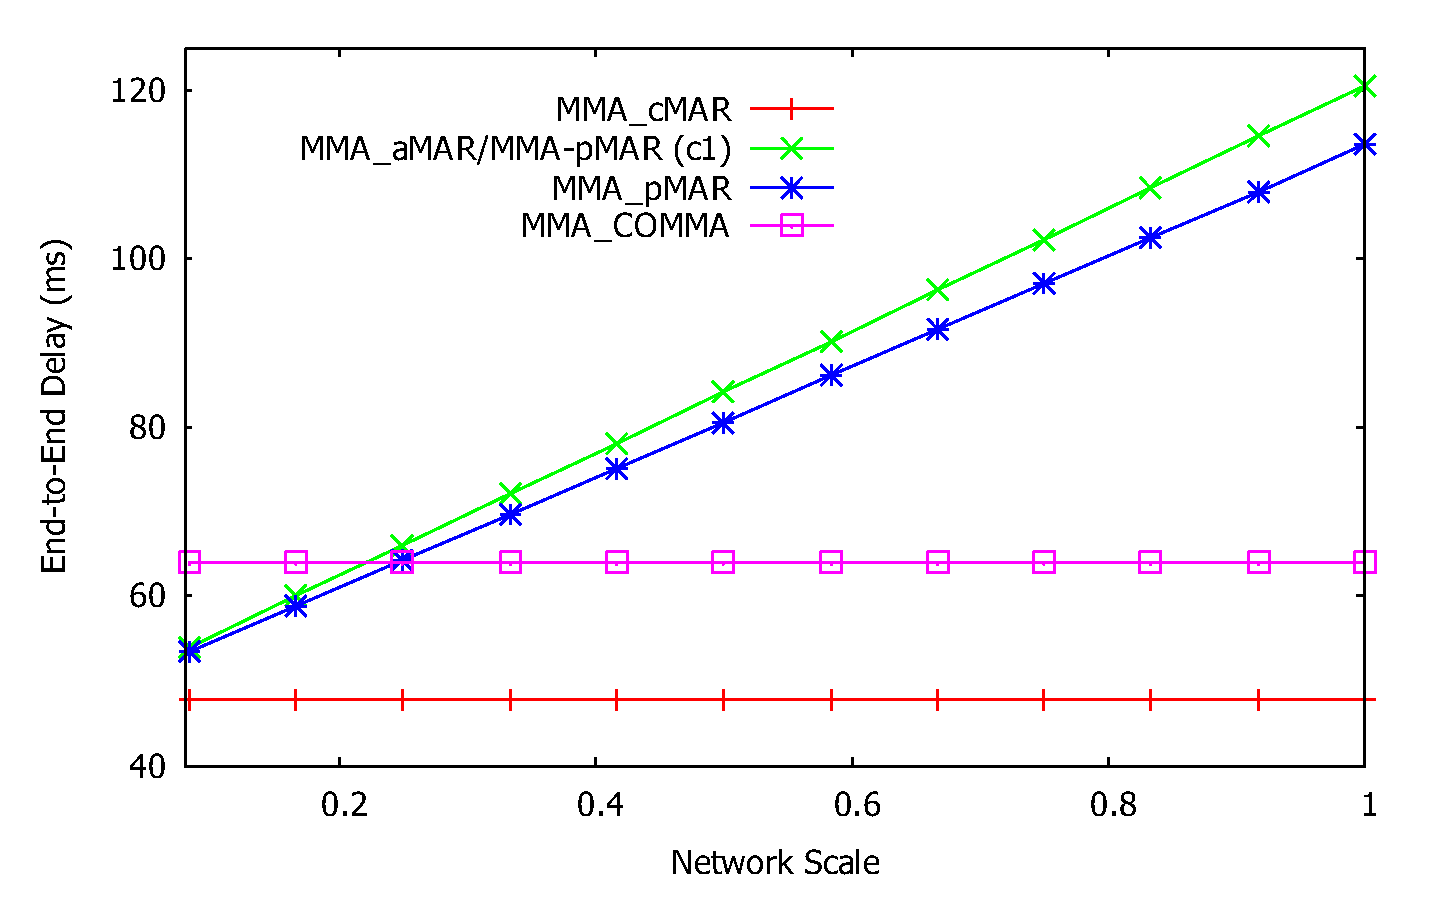
\includegraphics[width=0.50\textwidth]{./Part3/Chapter8/figures/c10_e2e_scale.eps}\label{fig:c10_e2e_scale}}\,
\subfloat[]{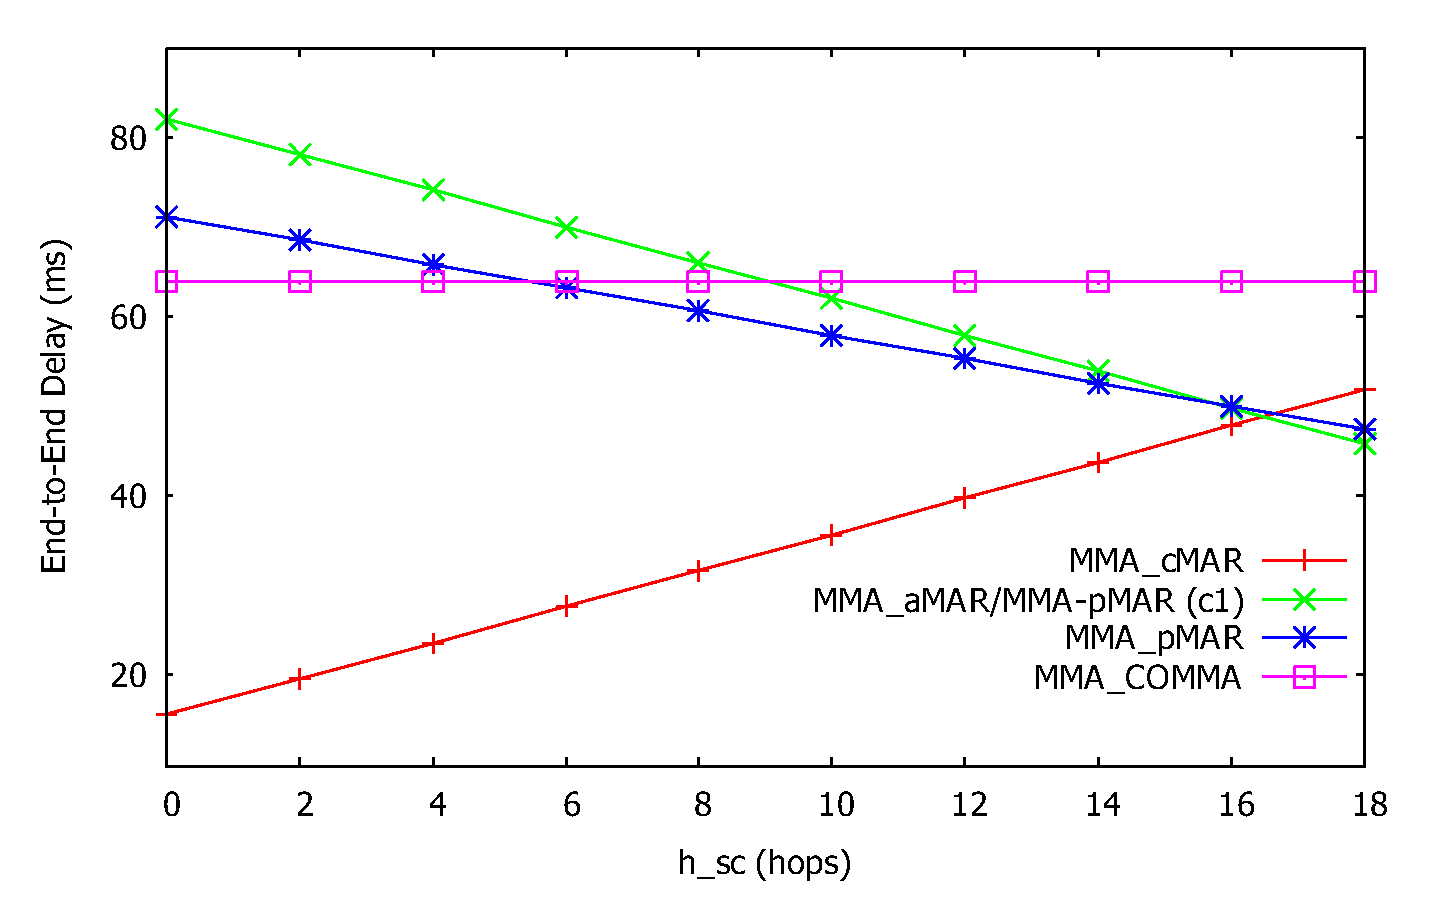
\includegraphics[width=0.50\textwidth]{./Part3/Chapter8/figures/c10_e2e_h_sc.eps}\label{fig:c10_e2e_h_sc}}
\caption[End-to-end delay.]{End-to-end delay as a function of: (a) $N_{mar}$, (b) $\psi$, (c) $h_{sc}$.}
\label{fig:c10_e2e}
\end{figure}
In conclusion, MMA\_pMAR is generally well suited for service interruption sensitive services. Moreover, the service disruption in the MMA\_aMAR is always greater than that in the MMA\_aMAR (c1). Thus, the increasing of service disruption time, which is caused by enabling the multiple upstream interfaces for the MLD proxy, can be considered as a trade-off between the service disruption time and the tunnel convergence problem. 

\subsubsection{End-to-End delay}
Now we investigate the impact of $N_{mar}$ on the end-to-end delay. Fig.~\ref{fig:c10_e2e_n_mar} shows the plot for the end-to-end delay versus the number of handover $N_{mar}$. As $N_{mar}$ increases ($h_{ac}$ increases) the end-to-end delay in case of MMA\_aMAR and MMA\_pMAR rapidly increases, while that in MMA\_cMAR and MMA\_COMMA is kept constant. Note that the end-to-end delay in MMA\_cMAR is kept below the value 50 ms. That means the MMA\_cMAR satisfies the strict requirement in terms of end-to-end delay (for real-time gaming \cite{e2e_requirement}). The delay in MMA\_pMAR(c1) is greater than that in MMA\_pMAR as a result of using the multiple upstream interfaces. As can be seen in Fig.~\ref{fig:c10_e2e_scale}, in general, the network scale has a similar impact on the end-to-end delay as $N_{mar}$. The major difference is that the increasing line of MMA\_pMAR in Fig.~\ref{fig:c10_e2e_scale} is faster than that in Fig.~\ref{fig:c10_e2e_n_mar}.

Then, $N_{mar}$ is set to a value of 6 (corresponding to the medium/long-lived and medium/high mobility scenario) while the value of $h_{sc}$ is varied. At this stage, we suppose that $h_{sa}$ + $h_{sc}$ is a fixed value, for example, 18 hops and $h_{sp}$ = $h_{sc}$. This scenario is used to illustrate the case where the source is extremely close to the aMAR (right-side of Fig.~\ref{fig:c10_e2e_h_sc}) or extremely close to the cMAR (left side of Fig.~\ref{fig:c10_e2e_h_sc}). As can be observed in Fig.~\ref{fig:c10_e2e_h_sc}, even when the source is very close to the aMAR ($h_{sa}$=2, $h_{sc}$=16), the MMA\_cMAR approach gives a better performance in terms of end-to-end delay than the others (lower is better). Thus, the impact of the mobility tunnel (cMAR-aMAR and cMAR-pMAR) on the end-to-end delay is obvious. In conclusion, the cMAR is generally well suited for the delay-sensitive flows. 
\begin{figure}[h!]
\centering
\subfloat[]{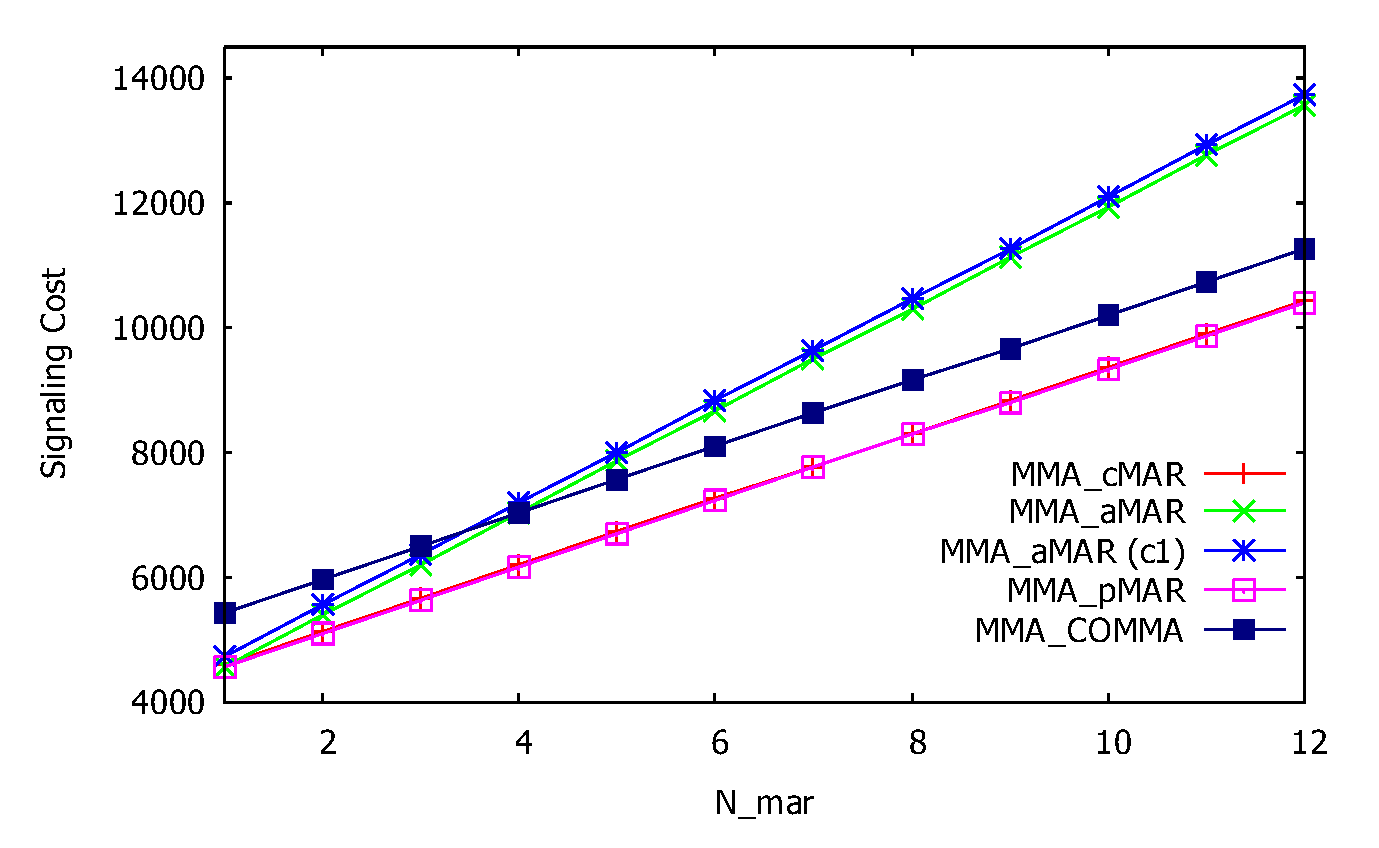
\includegraphics[width=0.50\textwidth]{./Part3/Chapter8/figures/c10_sc_n_mar.eps} \label{fig:c10_sc_n_mar}}
\subfloat[]{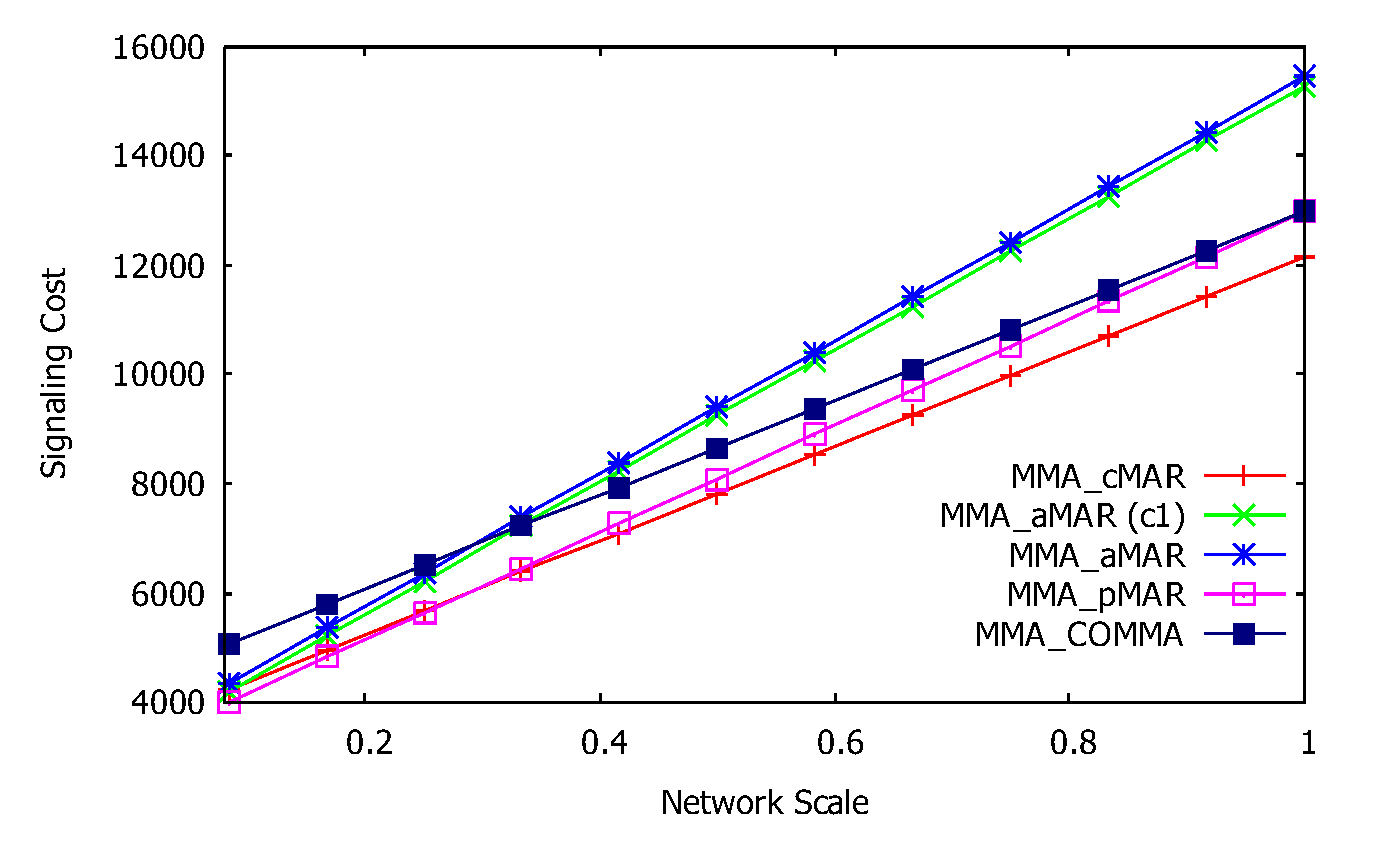
\includegraphics[width=0.50\textwidth]{./Part3/Chapter8/figures/c10_sc_scale.eps}\label{fig:c10_sc_scale}}\,
\subfloat[]{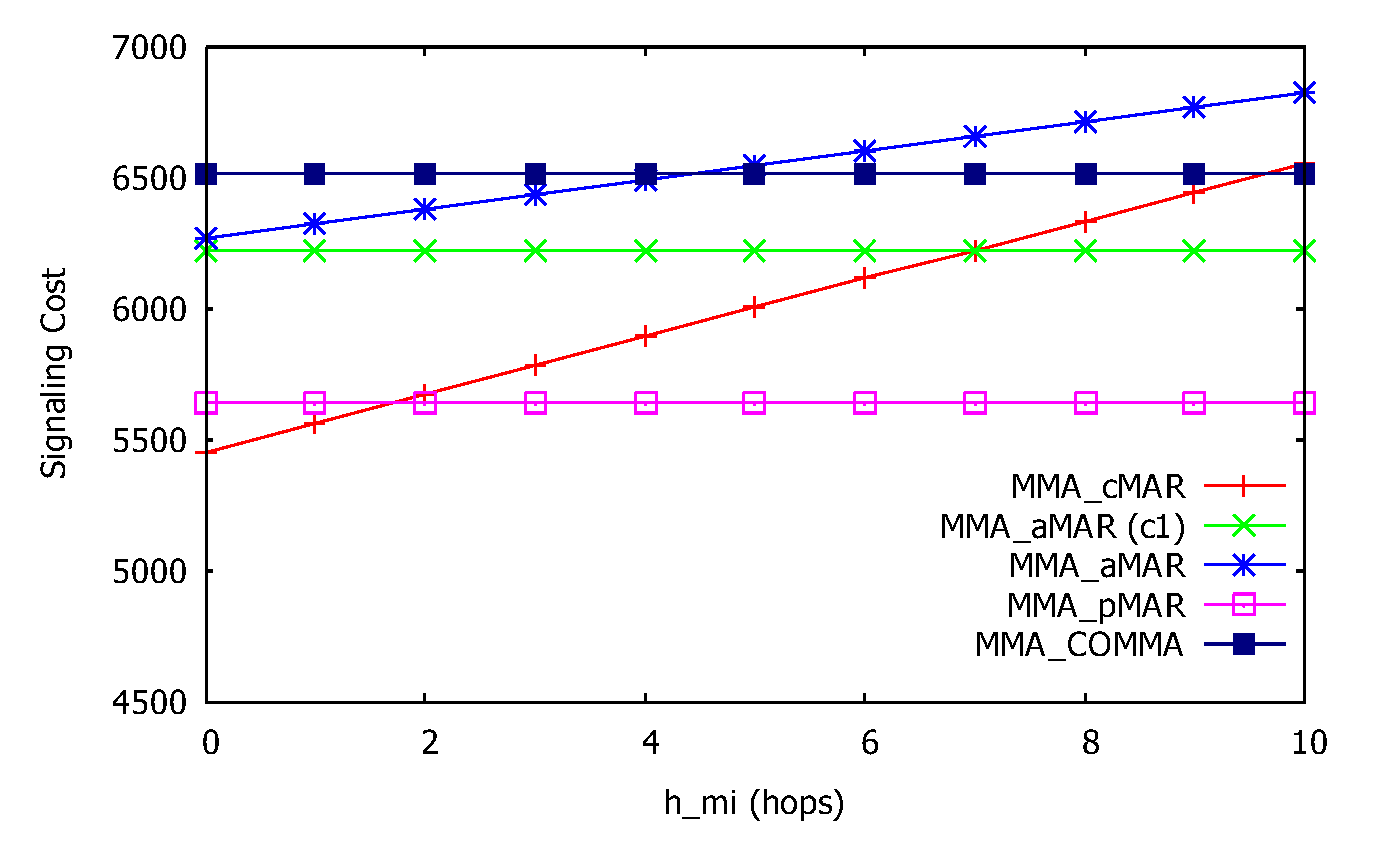
\includegraphics[width=0.50\textwidth]{./Part3/Chapter8/figures/c10_sc_h_mi.eps}\label{fig:c10_sc_h_mi}}
\caption[Signaling cost.]{Signaling cost as a function of: (a) $N_{mar}$, (b) $\psi$, (c) $h_{mi}$.}
\label{fig:c10_sc}
\end{figure}
\subsubsection{Signaling Cost}
Fig.~\ref{fig:c10_sc} shows the signaling cost as a function of  $N_{mar}$, $\psi$, and $h_{mi}$. In general, the signaling cost increases when $N_{mar}$ and $\psi$ increase. In Fig.~\ref{fig:c10_sc_n_mar}, the signaling cost in the MMA\_cMAR and MMA\_pMAR is lower than that in the other cases. In Fig.~\ref{fig:c10_sc_scale}, the signaling cost in the MMA\_pMAR is lowest when $\psi$ is small. Otherwise, it is the lowest in the MMA\_cMAR. In both cases, when $N_{mar}$ and $\psi$ are small enough, the signaling cost in case of MMA\_COMMA is getting highest. Otherwise, the signaling cost in case of MMA\_aMAR becomes highest. As can be seen in Fig.~\ref{fig:c10_sc_h_mi} (when $h_{mi}$ is varied), the MMA\_pMAR outperforms the others when $h_{mi}$ is greater than 2. 

\subsubsection{Packet Delivery Cost}
\begin{figure}[h!]
\centering
\subfloat[]{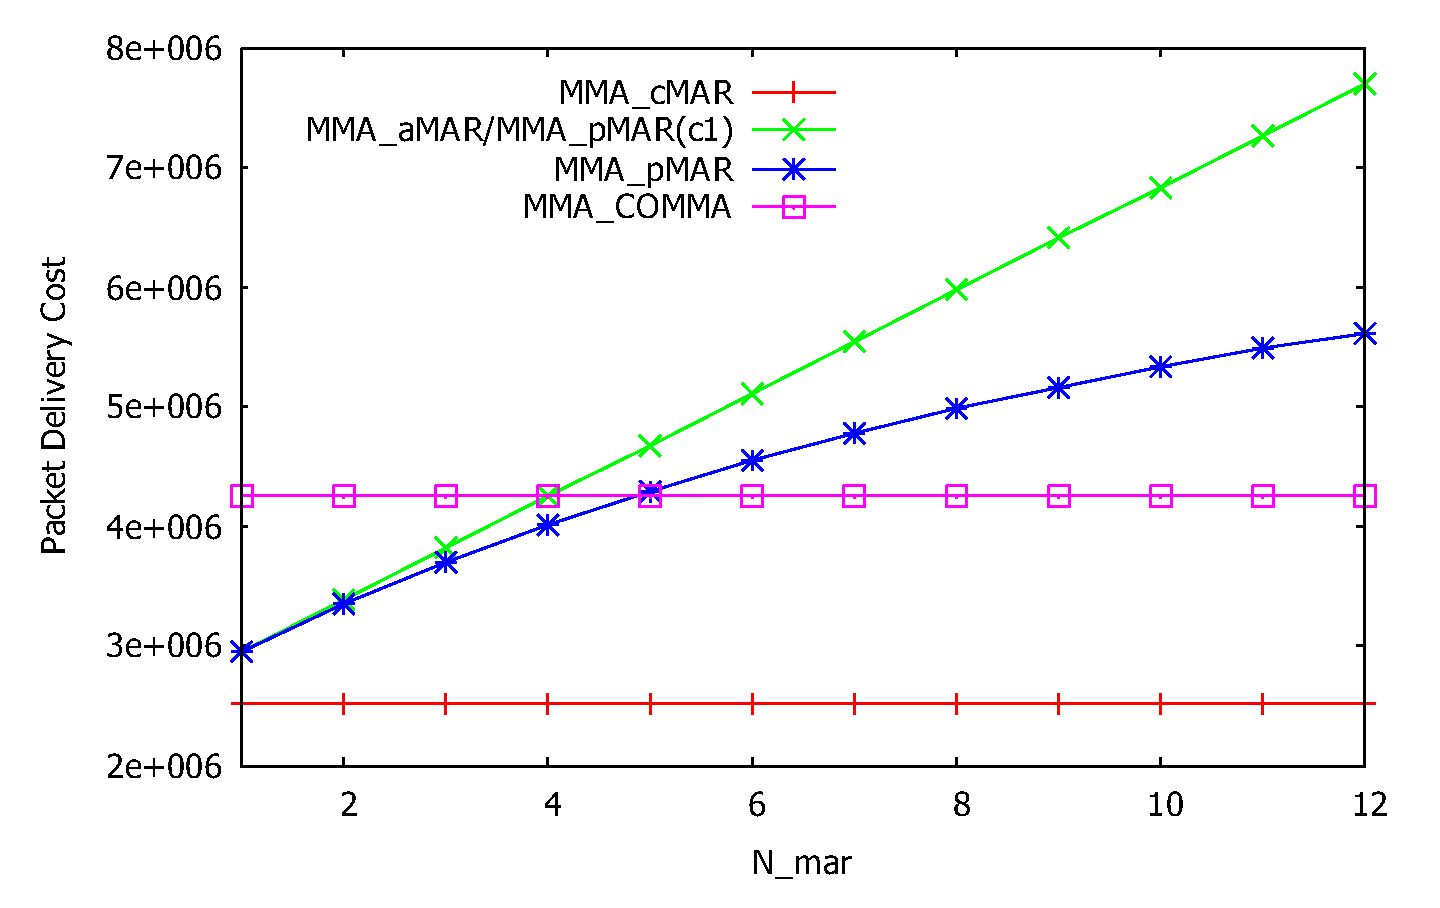
\includegraphics[width=0.50\textwidth]{./Part3/Chapter8/figures/c10_pc_n_mar.eps} \label{fig:c10_pc_n_mar}}
\subfloat[]{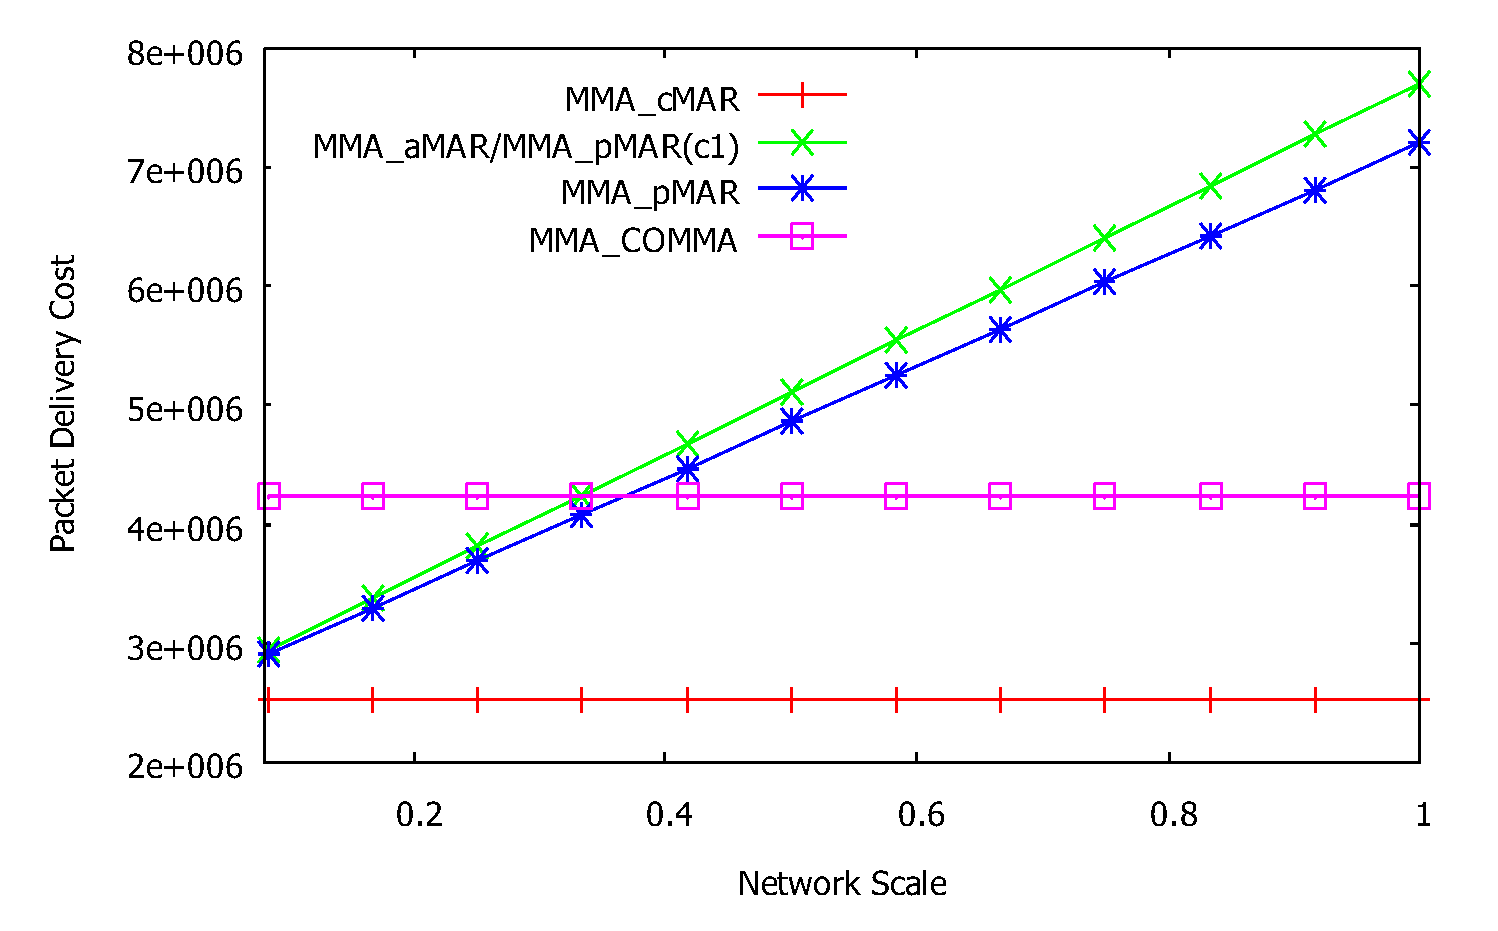
\includegraphics[width=0.50\textwidth]{./Part3/Chapter8/figures/c10_pc_scale.eps}\label{fig:c10_pc_scale}}\,
\subfloat[]{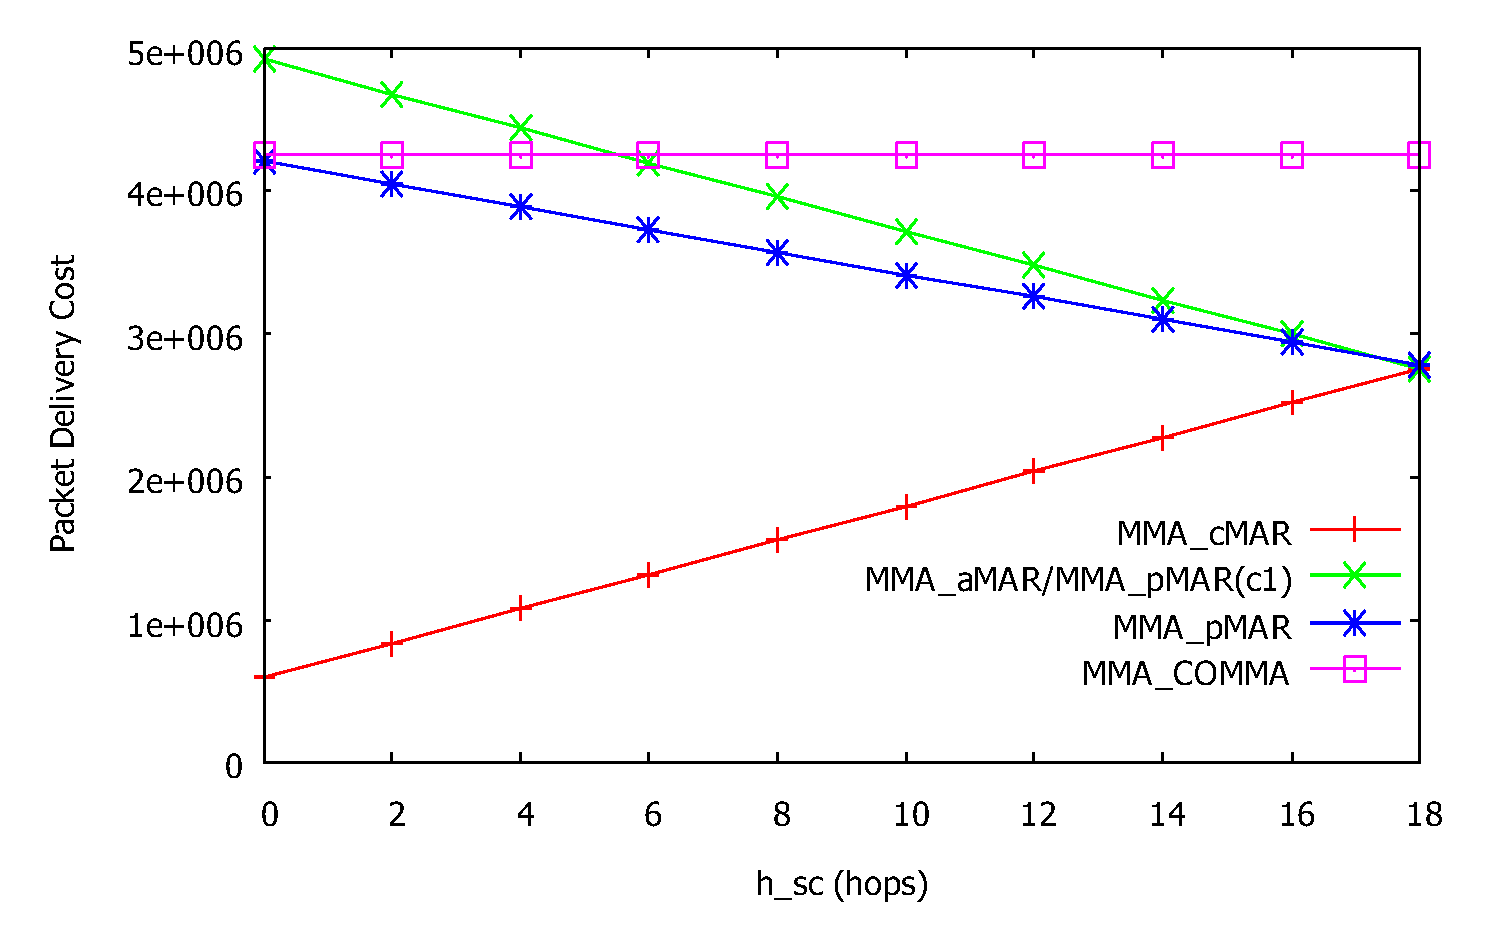
\includegraphics[width=0.50\textwidth]{./Part3/Chapter8/figures/c10_pc_h_sc.eps}\label{fig:c10_pc_h_sc}}
\caption[Packet delivery cost.]{Packet delivery cost a function of: (a) $N_{mar}$, (b) $\psi$, (c) $h_{sc}$.}
\label{fig:c10_pc}
\end{figure}

Similar to the end-to-end delay, the packet delivery cost (as a function of $N_{mar}$ and  $\psi$) in case of MMA\_cMAR and MMA\_COMMA is kept constant while that in case of MMA\_aMAR and MMA\_pMAR is greatly increased. Fig.~\ref{fig:c10_pc_h_sc} shows the packet delivery cost as a function of $h_{sc}$ when $h_{sa} + h_{sc}$ is fixed (18 hops). It appears clearly that the packet delivery cost in MMA\_cMAR is definitely lower than that in the others, even when the source is very close to the aMAR. Also, we can observe that this cost in case of MMA\_pMAR(c1) is greater than that in MMA\_pMAR as a result of enabling the multiple upstream interfaces. 

\subsubsection{Tunneling Cost}
\begin{figure}[h!]
 	\begin{center} 
		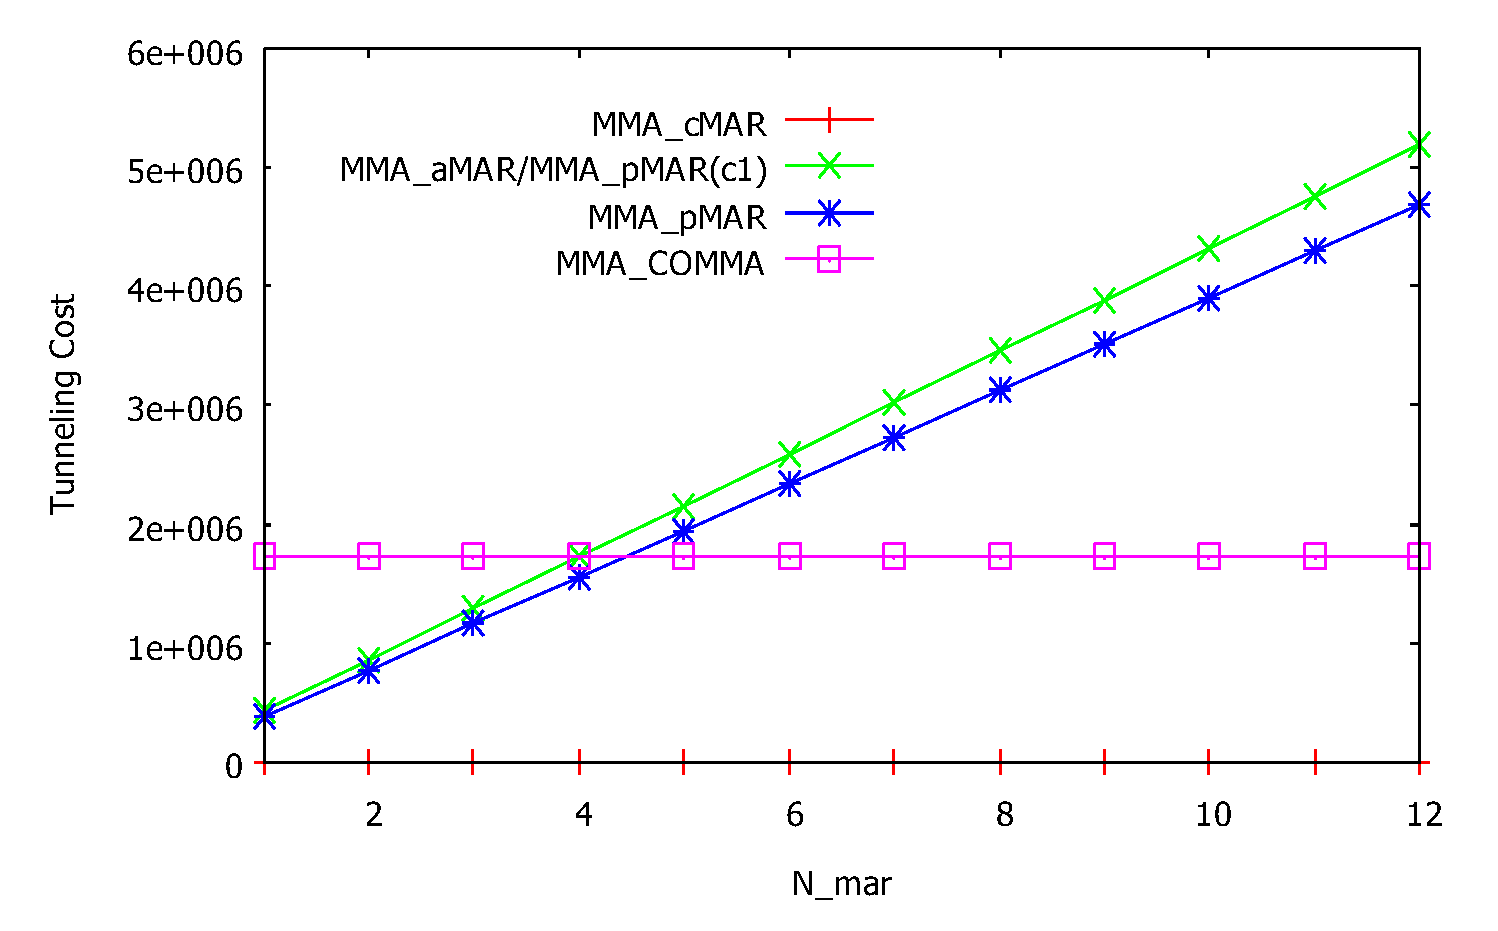
\includegraphics[width=0.50\textwidth]{./Part3/Chapter8/figures/c10_tc_n_mar.eps}
		\caption[Tunneling cost.]{Tunneling cost as a function of $N_{mar}$.}
		\label{fig:c10_tc_n_mar}
	\end{center}
\end{figure}

Regarding the tunneling cost, Fig.~\ref{fig:c10_tc_n_mar} plots the tunneling cost as a function of $N_{mar}$. The MMA\_cMAR does not introduce any tunneling overhead, while the tunneling cost in the MMA\_COMMA is fixed. On the other hand, it is significantly increased as $N_{mar}$ increases in case of MMA\_aMAR and MMA\_pMAR. Again, by applying the multiple upstream interfaces, the tunneling cost in case of MMA\_pMAR slightly increases.

\subsubsection{Packet Loss}
\begin{figure}[h!]
\centering
\subfloat[]{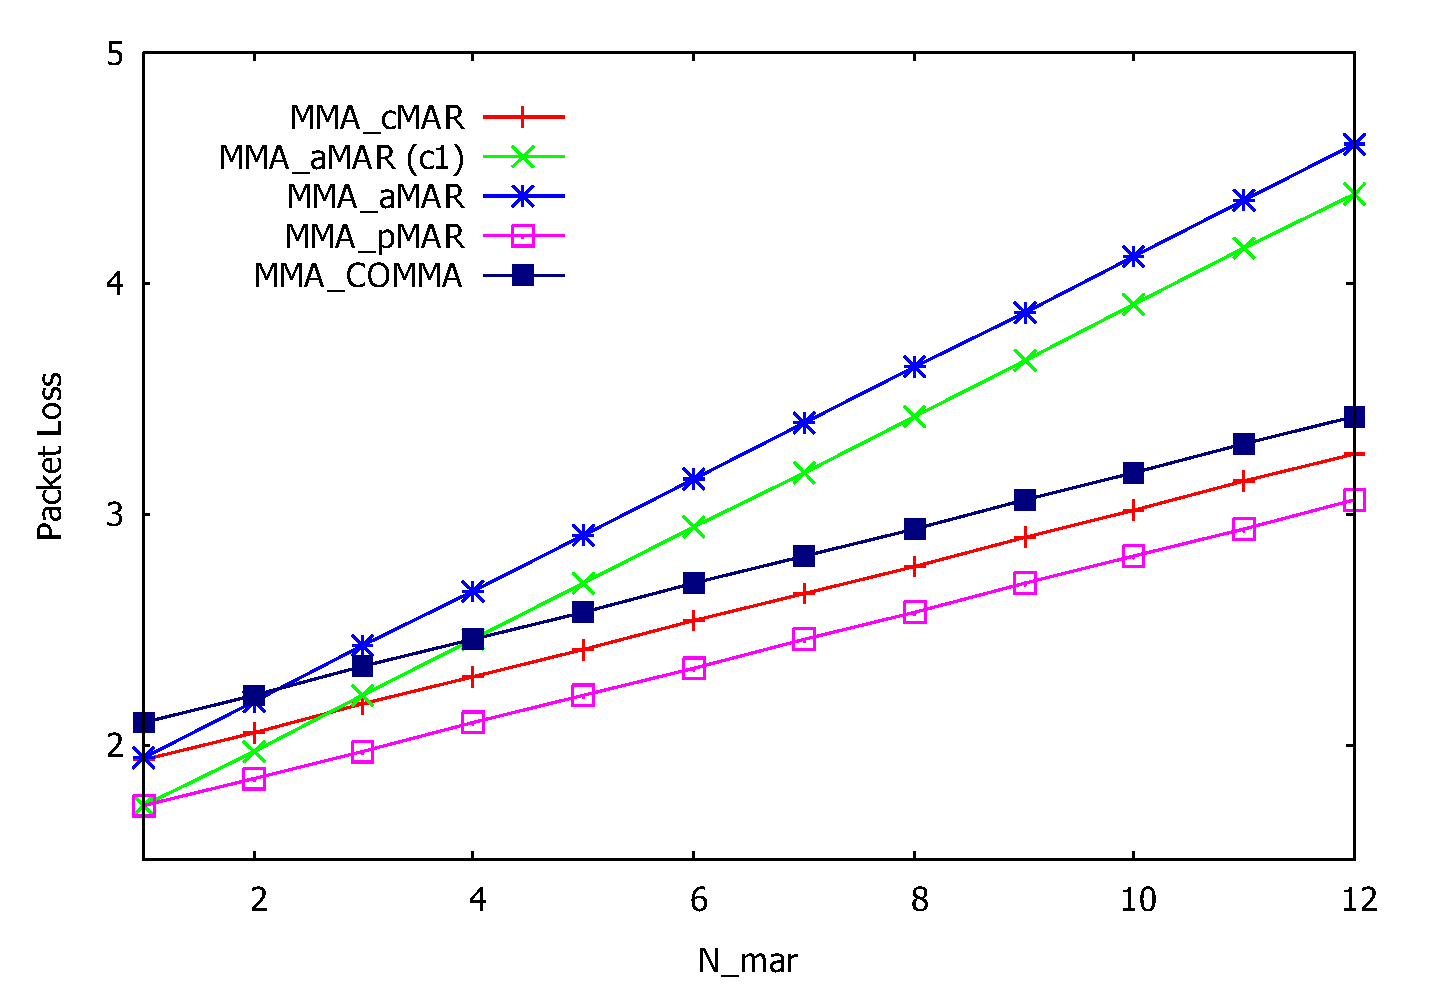
\includegraphics[width=0.37\textwidth]{./Part3/Chapter8/figures/c10_pl_n_mar.eps} \label{fig:c10_pl_n_mar}}
\subfloat[]{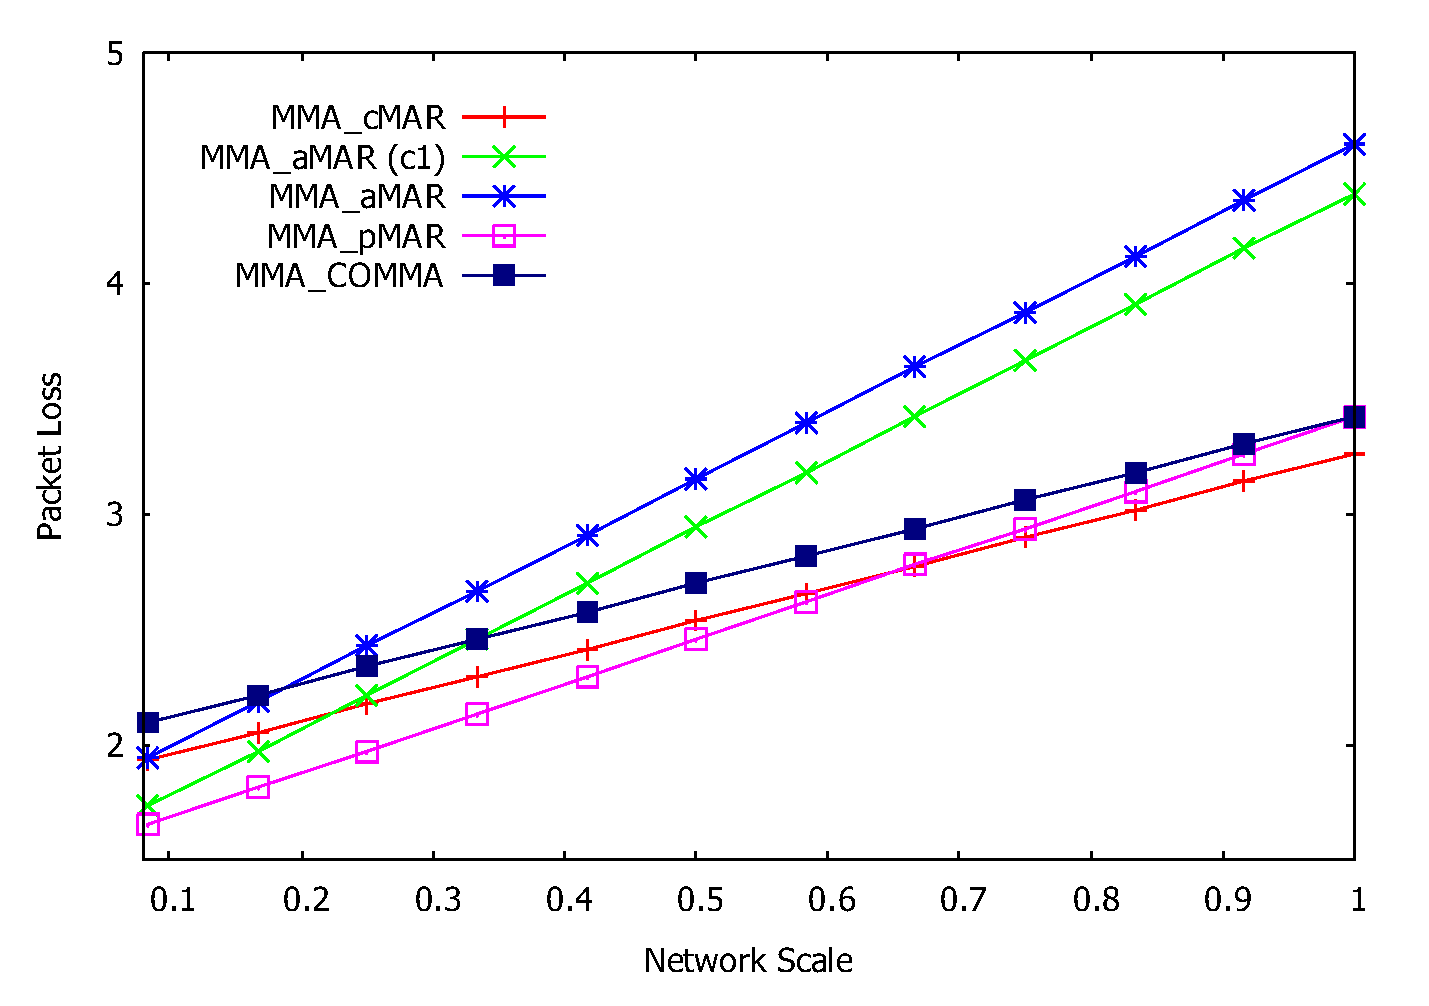
\includegraphics[width=0.37\textwidth]{./Part3/Chapter8/figures/c10_pl_scale.eps}\label{fig:c10_pl_scale}}
\subfloat[]{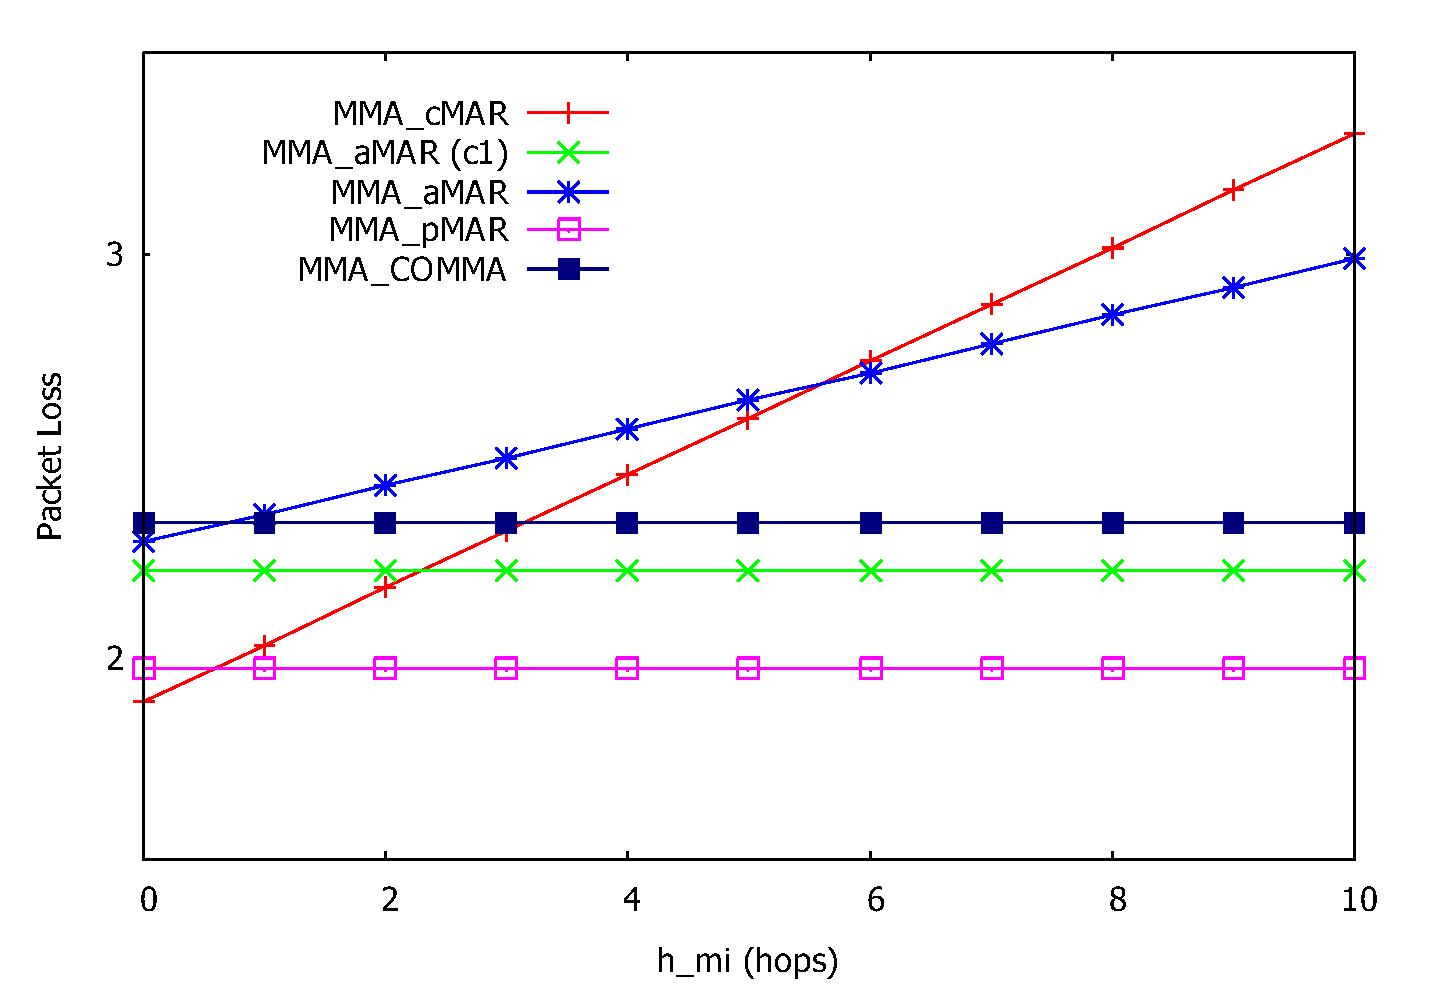
\includegraphics[width=0.37\textwidth]{./Part3/Chapter8/figures/c10_pl_h_mi.eps}\label{fig:c10_pl_h_sc}}
\caption[Packet Loss.]{Packet loss as a function of: (a) $N_{mar}$, (b) $\psi$, (c) $h_{mi}$.}
\label{fig:c10_pl}
\end{figure}
Fig.~\ref{fig:c10_pl} illustrates the packet loss. Since the number of lost packets during handover is directly proportional to the service disruption time, the shape of the curves is similar to that in Fig.~\ref{fig:c10_sd}. 

\subsubsection{Expected Number of Handovers}
Now we investigate the relation between number of handovers $N_{mar}$, the velocity and the MAR's coverage area. It is assumed that the subnet residence time (MAR subnet) and the session duration are random variables which follow an exponential distribution with mean value 1/$\mu_{c}$ and 1/$\mu_{s}$, respectively. According to \cite{HO_comparison_Makaya}, the expected number of handovers is defined as \\
\begin{equation}
  E=\frac{\mu_{c}}{\mu_{s}}.
\end{equation}

In this chapter, we consider the case where the MN always moves from MAR to MAR as if they were linearly deployed (the user is moving further away from the first attached MAR and never attaches back to a previously visited MAR, representing the worst-case scenario). Thus, $N_{mar} =  E$. Assuming that MAR's coverage area is circular with radius R, then, $\mu_{c}$ is calculated as \cite{HO_comparison_Makaya} \\
\begin{equation}
\mu_{c}=\frac{2 \upsilon}{\pi R},
\end{equation}
where $\upsilon$ is the average velocity of the MN.

\begin{figure}[h!]
\centering
\subfloat[]{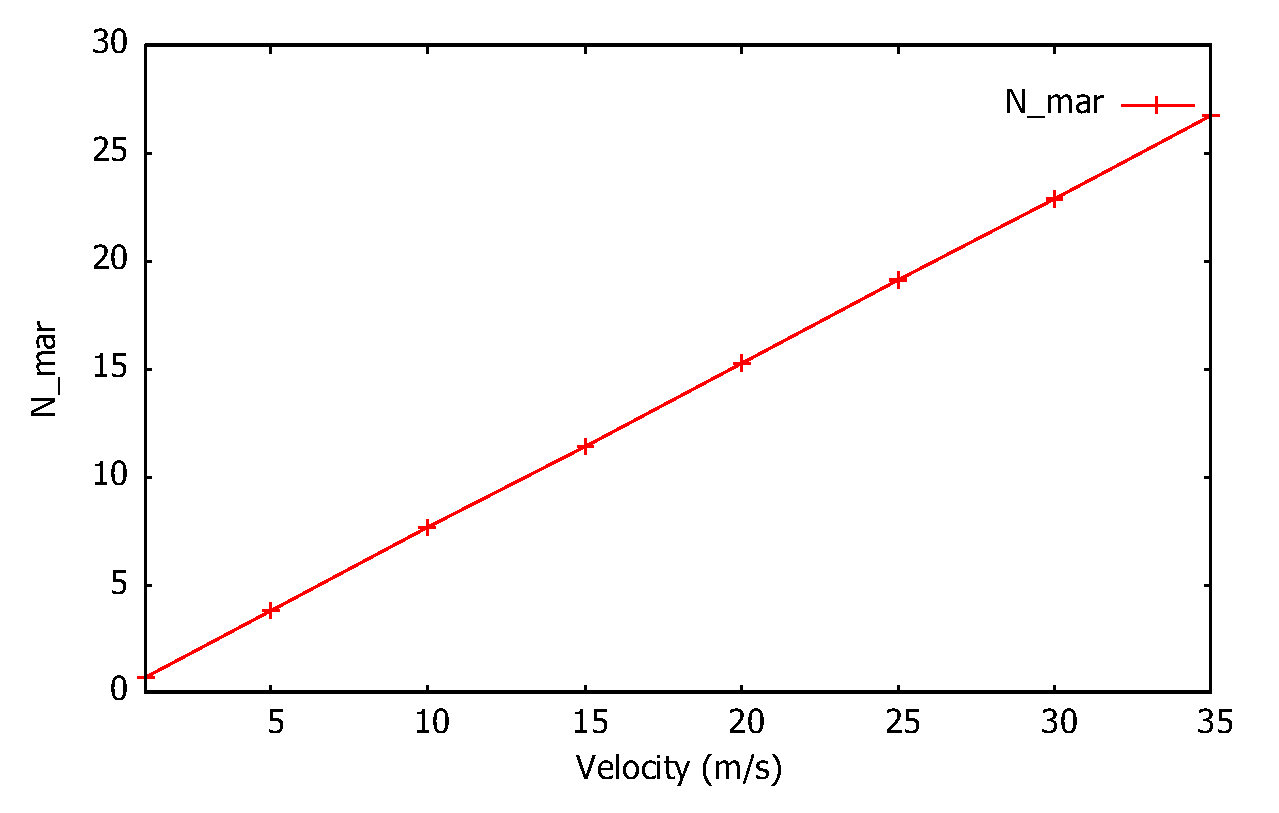
\includegraphics[width=0.37\textwidth]{./Part3/Chapter8/figures/c10_v.eps} \label{fig:c10_v}}
\subfloat[]{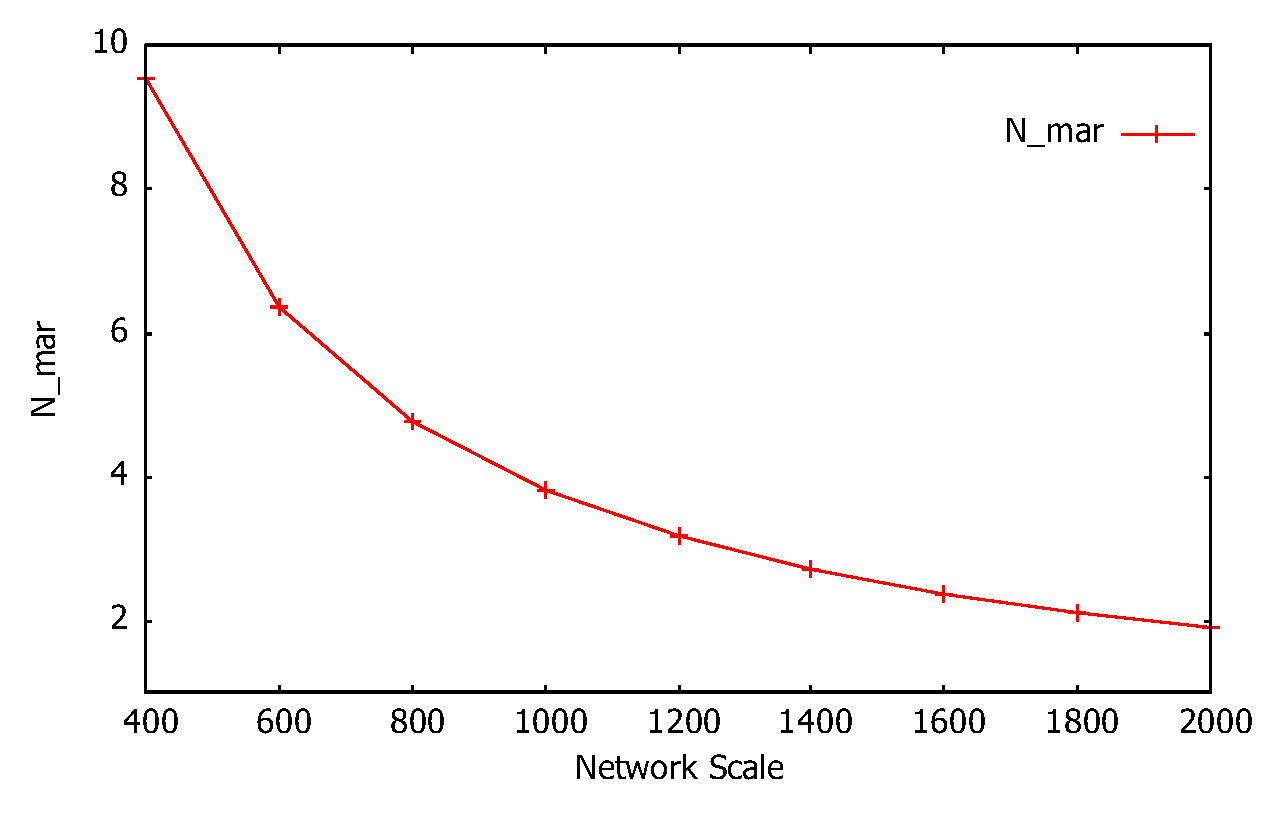
\includegraphics[width=0.37\textwidth]{./Part3/Chapter8/figures/c10_r.eps}\label{fig:c10_r}}
\subfloat[]{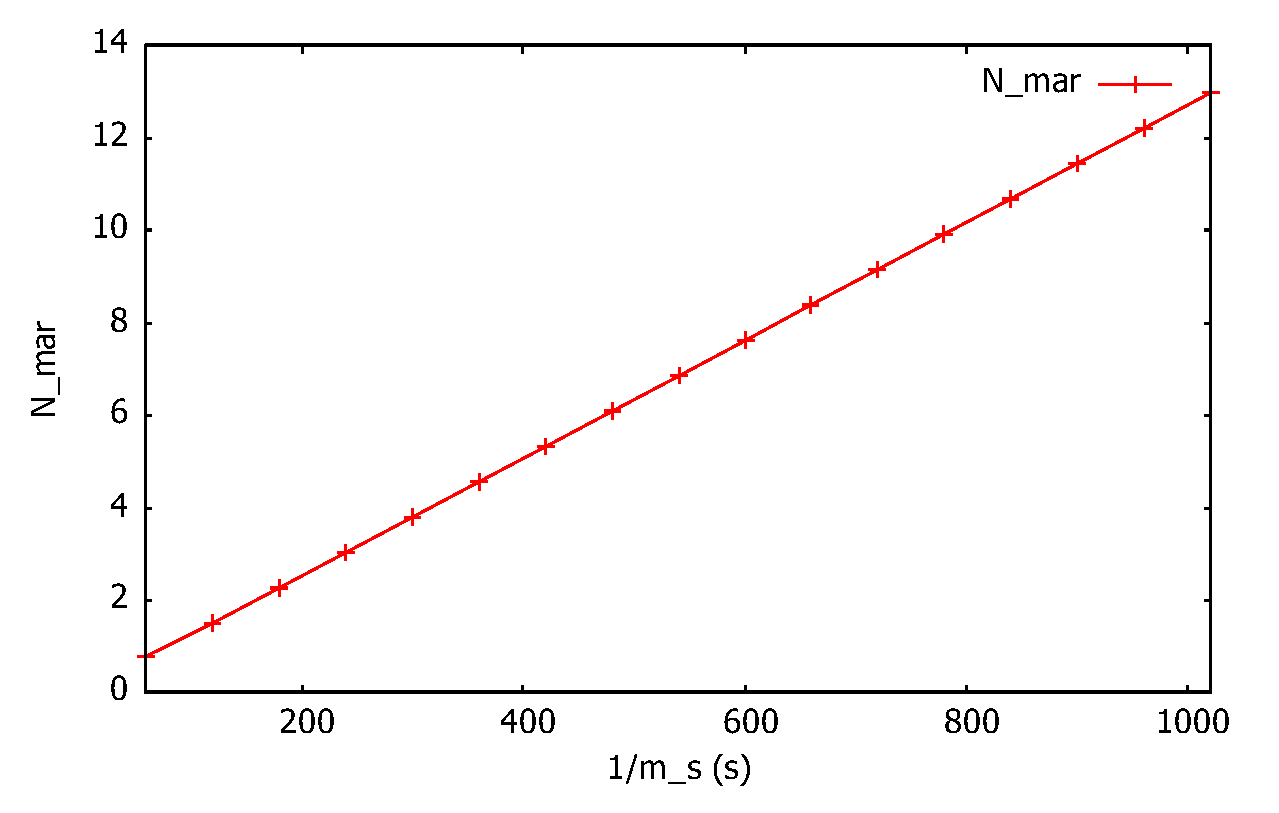
\includegraphics[width=0.37\textwidth]{./Part3/Chapter8/figures/c10_mc.eps}\label{fig:c10_mc}}
\caption[Expected number of handovers.]{$N_{mar}$ as a function of: (a) velocity, (b) subnet radius, (c) 1/$\mu_{s}$.}
\label{fig:c10_n_mar}
\end{figure}

Fig.~\ref{fig:c10_v} depicts $N_{mar}$ as a function of the velocity when 1/$\mu_{s} $ is fixed to 600s. As the velocity increases, $N_{mar}$ increases. Thus, the high value of $N_{mar}$ corresponds to the high mobility scenario. Then we take a look at the impact of subnet radius R on the value of $N_{mar}$. The higher value of R means the size of the access network is bigger. As R increases, the residence time in a subnet decreases, thus the  number of handover ($N_{mar}$) decreases (see Fig.~\ref{fig:c10_r}). Fig.~\ref{fig:c10_mc} plots $N_{mar}$ as a function of 1/$\mu_{s}$ when $\upsilon$ and $R$ are set to 10m/s and 500m, respectively. As 1/$\mu_{s}$  increases, $N_{mar}$ increases. In our analysis, the high value of 1/$\mu_{s}$ illustrates the long-lived flow scenario. 

\subsection{Conclusion of the Quantitative Analysis}
From the performance analysis and numerical results, we conclude that none of the approaches is always better than the others. For example, the MMA\_pMAR generally is a good choice when considering the multicast service disruption; the MMA\_cMAR, in contrast, is a better choice regarding the end-to-end delay. The other approaches can be the most suitable, however, in a specific situation. The performance analysis also gives an idea of using a common MMA (COMMA) which serves as an only multicast anchor for all the nodes in the domain, thus, reflecting the PMIPv6 deployment. Although this approach introduces an acceptable performance, e.g., when $N_{mar}$ and $\psi$ are small, COMMA poses a bottleneck and a single point of failure. It is also not a good choice when a local content is available. As a result, the comparison between the MMA\_COMMA and the default mode gives the idea of the performance of DMM with respect to PMIPv6 regarding multicast service. 

Basically, the performance of the approaches depends on such factors as the number of handovers ($N_{mar}$, which can be considered as a function of the velocity and the subnet radius), the network scale ($\psi$), the position of the source ($h_{sc}$, $h_{sa}$) and the listener density ($h_{mi}$). Those are the reasons why a fixed MMA is not a good strategy. In addition, the daily mobile users spend up to 62\% of their time at home and work (in general, typical location) \cite{cisco_connected_lives}. Thus, in some cases, the typical location would also be a good candidate. Even the mobility anchors are distributed, some of them are overloaded more than the others \cite{anchor_selection}. As a result, a per-flow multicast support should be provided. 

In the next section, a dynamic multicast mobility anchor mechanism will be introduced. Based on the collected contexts, the MMA will be selected dynamically in order to meet a set of requirements. From a service point of view, it helps satisfy the requirements in terms of service disruption and delay, especially when considering real-time services. It also provides a mechanism to better distribute the load among MARs. Other issues such as packet duplication and leave latency (waste of resource) can be reduced. The MMA selection takes into account not only the multicast service context (e.g., interruption-sensitive and delay-sensitive services) but also the mobile node’s mobility context and the network context (such as the load of MARs and the multicast channel policy), thus enabling a per-flow multicast support. In other words, each multicast flow can be treated differently up on the contexts. The MMA selection can be made dynamically when a multicast flow is initiated or when the listener performs a handover thanks to the MLD proxy supporting multiple upstream interfaces.

\section{Dynamic Multicast Mobility Anchor Selection} \label{c10:dmma}
To mitigate the issues caused by the movement of a listener following the multicast default mode, this section proposes a mechanism which allows dynamically selecting and using the appropriate MMA among the candidates, namely dynamic multicast mobility anchor mechanism or DMMA. This idea follows the assumption of the DMM protocol specified by the IETF \cite{dmm-best-practice}. The MMA selection can be made whenever the listener performs a handover or a multicast flow is initiated. As a result, the tunnel convergence problem is completely avoided. 

To dynamically select the appropriate MMA, different contexts should be taken into account as the multicast service context (e.g., interruption-sensitive, delay-sensitive, and long-lived/short-lived flow), the MN's mobility context (high/low mobility)\footnote{The MMA selection also depends on the role of the node in the multicast session (source or listener).}, and the network context (like load of MARs, geographical proximity, and multicast channel policy). Each context can be assigned with a priority number. For example, a lower value indicates the more important context. 

At this stage, similar to the default mode, when a listener initiates a multicast flow, the cMAR will act as the MMA for this flow (the multicast traffic will be received directly from the native multicast infrastructure). This means the MMA selection in the initial phase will be left for future works. For a handover flow, the multicast traffic can be received from the aMAR, the pMAR, the cMAR, or even an MAR in which the multicast channel is already available, or a less loaded MAR so as to meet a set of requirements. In addition, we consider the typical location (tMAR) corresponding to the MMA\_tMAR approach. 

Our solution is not only for the service disruption and the end-to-end delay issues, but also for another multicast related issues. Thus, it can offer such benefits as:
\begin{itemize}
\item \textit{A complete solution} for most of the multicast listener mobility-related issues (including service disruption, tunnel convergence problem, leave latency (network resource waste), sub-optimal routing and packet loss);
\item \textit{Route optimization}: The multicast flows will be routed in a better route since they do not always pass through their mobility anchor. 
\item \textit{Tunnel convergence problem avoidance}: This solution can fully resolve the tunnel convergence problem;
\item \textit{Dynamic utilization of mobility tunnel}: The utilization of mobility tunnel for the ongoing multicast sessions is enabled in appropriate cases e.g., for remote content, or for a channel with strict delay requirements;
\item \textit{Effective tunnel management}: In a DMM environment, it is unfeasible to pre-establish all the tunnels between MARs since the number of MARs is supposed to be large. By enabling the multiple upstream interfaces in DMM, it may cause the complex tunnel management (e.g., maintenance of the tunnel and keep alive signaling). Thus, the proposed solution, which is based on the multicast mobility management module, can help to solve this issue;
\item \textit{Multicast flow load distribution}: Since the MMA selection takes the current load of the MARs into account, it helps better distribute the multicast traffic load among MARs. 
\item \textit{Centralized channel management}: The central entity (Multicast Control Entity, or MCE) collects and manages the considered contexts (e.g., the multicast channels and their scope (local or remote), thus enhancing the control of network providers;
\item \textit{Possibility to be applied with multicast source mobility};
\item \textit{Compatibility with unicast mobility}.
\end{itemize}

\subsection{Considered Contexts}
\paragraph{Multicast service context}
When services are sensitive to interruption or packet loss, the service disruption time should be minimized. For instance, it should be less than 300ms for a real-time service, while 500ms for a normal one \cite{interruption_requirements}. For the end-to-end delay-sensitive service, the long mobility tunnel, which can result in a high end-to-end delay, should be avoided. ITU-T Recommendation G.114 \cite{itu-t} suggests that if one-way transmission time for connection delays can be kept below 150ms, most applications will experience a transparent interactivity. Moreover, the long-lived flows may perform many handovers while the short-lived ones seem to be initiated and terminated at the same MAR without performing any handover. Even if a short-lived flow could make it, it is expected that the flow does not last long after the handover. 

\paragraph{Mobile node context}
A mobile node with high mobility performs frequent handovers. In this case, almost all ongoing multicast flows are the handover ones which may cause the longer tunnel. If the multicast traffic is always routed through the aMAR, the longer dwell time is, the more serious the impact will be. Also, the number of anchors and tunnels may be increased. On the contrary, for the low mobility node, the MN is expected to stay at one or several MARs most of the time. Since the users spend most Internet usage time at their typical locations (tMAR), in some cases, the tMAR can be a good candidate. 

\paragraph{Network context}
The MMA selection can also be based on several network contexts such as current load of the MARs, geographical proximity of the MAR to the MN as well as the multicast channel policy\footnote{The network operator can define the channel policy in which some channels should be received directly from the native multicast infrastructure (to gain benefit from local content) while the others from their anchor MAR \cite{Thinh_VTC}}. For example, when the load of MAR is high, it may cause long delays and packet losses if it is selected as the multicast anchor. In this case, the least loaded MAR (among the MARs having the multicast forwarding state for this channel) can be a potential candidate. The reason lies in the fact that if the channel is already available at the selected MAR, the service disruption time can be minimized (no need extra time to join the multicast channel). Also, with a negligible increase of load, this MAR can forward the traffic to the cMAR \cite{developing_ip_multicast}.

\subsection{Architecture Description}
In order to collect and manage the considered contexts, a network entity, called Multicast Control Entity (MCE) is introduced. The MCE can be collocated with the CMD. The MAR periodically updates the MN context and MAR's current load to the MCE by using an extension of PBU/PBA (or an extension of the Heartbeat messages \cite{heartbeat}). The MCE also manages all the multicast channel in the domain for network policy configuration. The service context can be defined based on the QoS class. 

Residing in the MAR, the multicast mobility management module (MUMO) takes responsibility for all actions related to the multicast mobility. The structure of this module is depicted in Fig.~\ref{fig:multicast_module} and briefly described as follows: 

\begin{figure}[t!]
 	\begin{center} 
		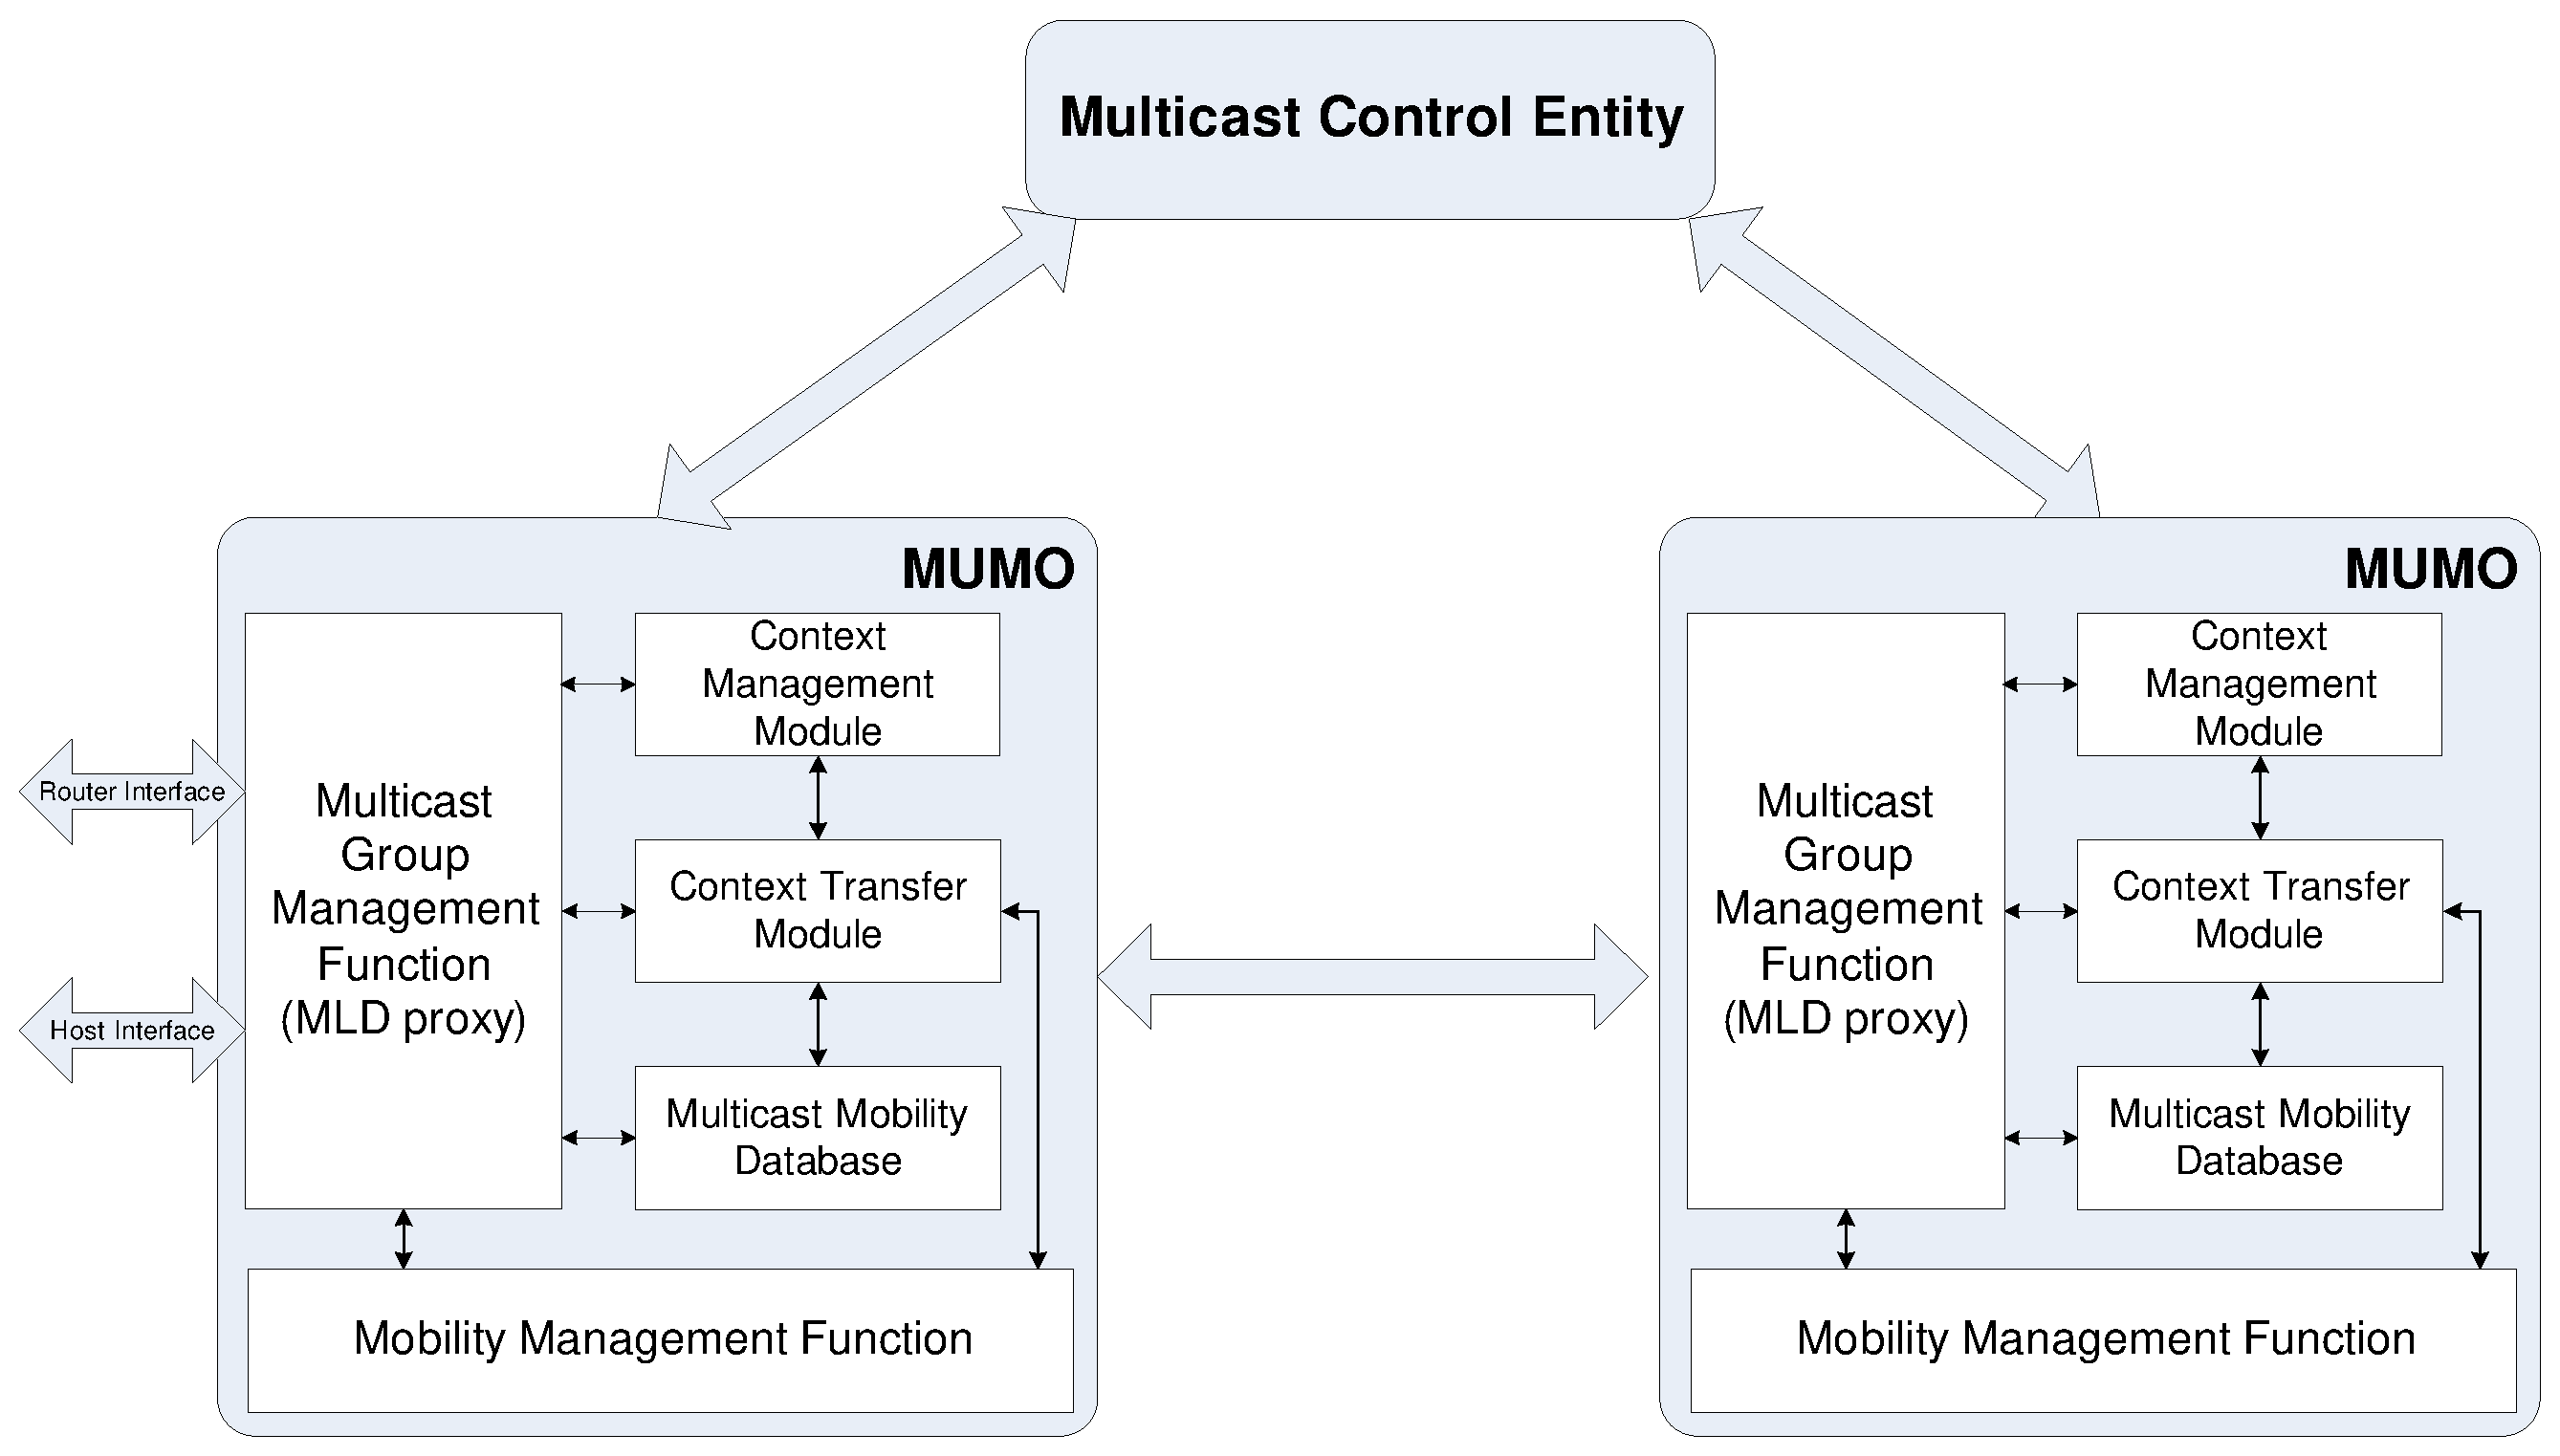
\includegraphics[width=0.90\textwidth]{./Part3/Chapter8/figures/c10_mume.eps}
		\caption{Multicast mobility management module (MUMO) in the MAR.}
		\label{fig:multicast_module}
	\end{center}
\end{figure}

\begin{itemize}
\item The multicast group management function (MGMF) refers to the multicast group management operations and information storage, which is developed based on the MLD proxy with multiple upstream interfaces\footnote{This module can also be relied on the multicast router function e.g., MRDv6.}. This module also supports the multicast explicit tracking function in order to keep a per-host multicast membership state \cite{explicit_tracking}. It is done based on its Multicast Mobility Database (MMD), which stores entries with the following information: i) MN's identifier (MN\_ID); MN's address; and multicast subscriptions (aligned with the structure of MLD multicast information). Besides, it holds a counter structure for the number of listeners per IP multicast channel, allowing it to identify when a node is the last subscriber of a group. This information is in particular essential for a proper multicast context transfer operation.
\item The context management function (CMF) communicates with the MCE to retrieve the channel configuration information including the address of the corresponding MMA, and MMA type (i.e., the previous, anchor, and current MAR or another). Based on this information, MLD proxy configures its upstream interfaces towards the corresponding MAR. 
\item The multicast context transfer function (MCTF) is responsible for exchanging the MN's multicast subscription information between MARs. So that the new MAR can join the on-going flows in advance to minimize the service disruption. 
\item The mobility management function (MMF) resembles the mobility protocol stack. It is responsible for assigning and maintaining the IP connectivity of an MN roaming inside the DMM domain. In other words, it is responsible for all the mobility management-related actions.  
\end{itemize}
\subsection{Operations of the Solution}
\begin{figure}[tb!] 
  \begin{center} 
    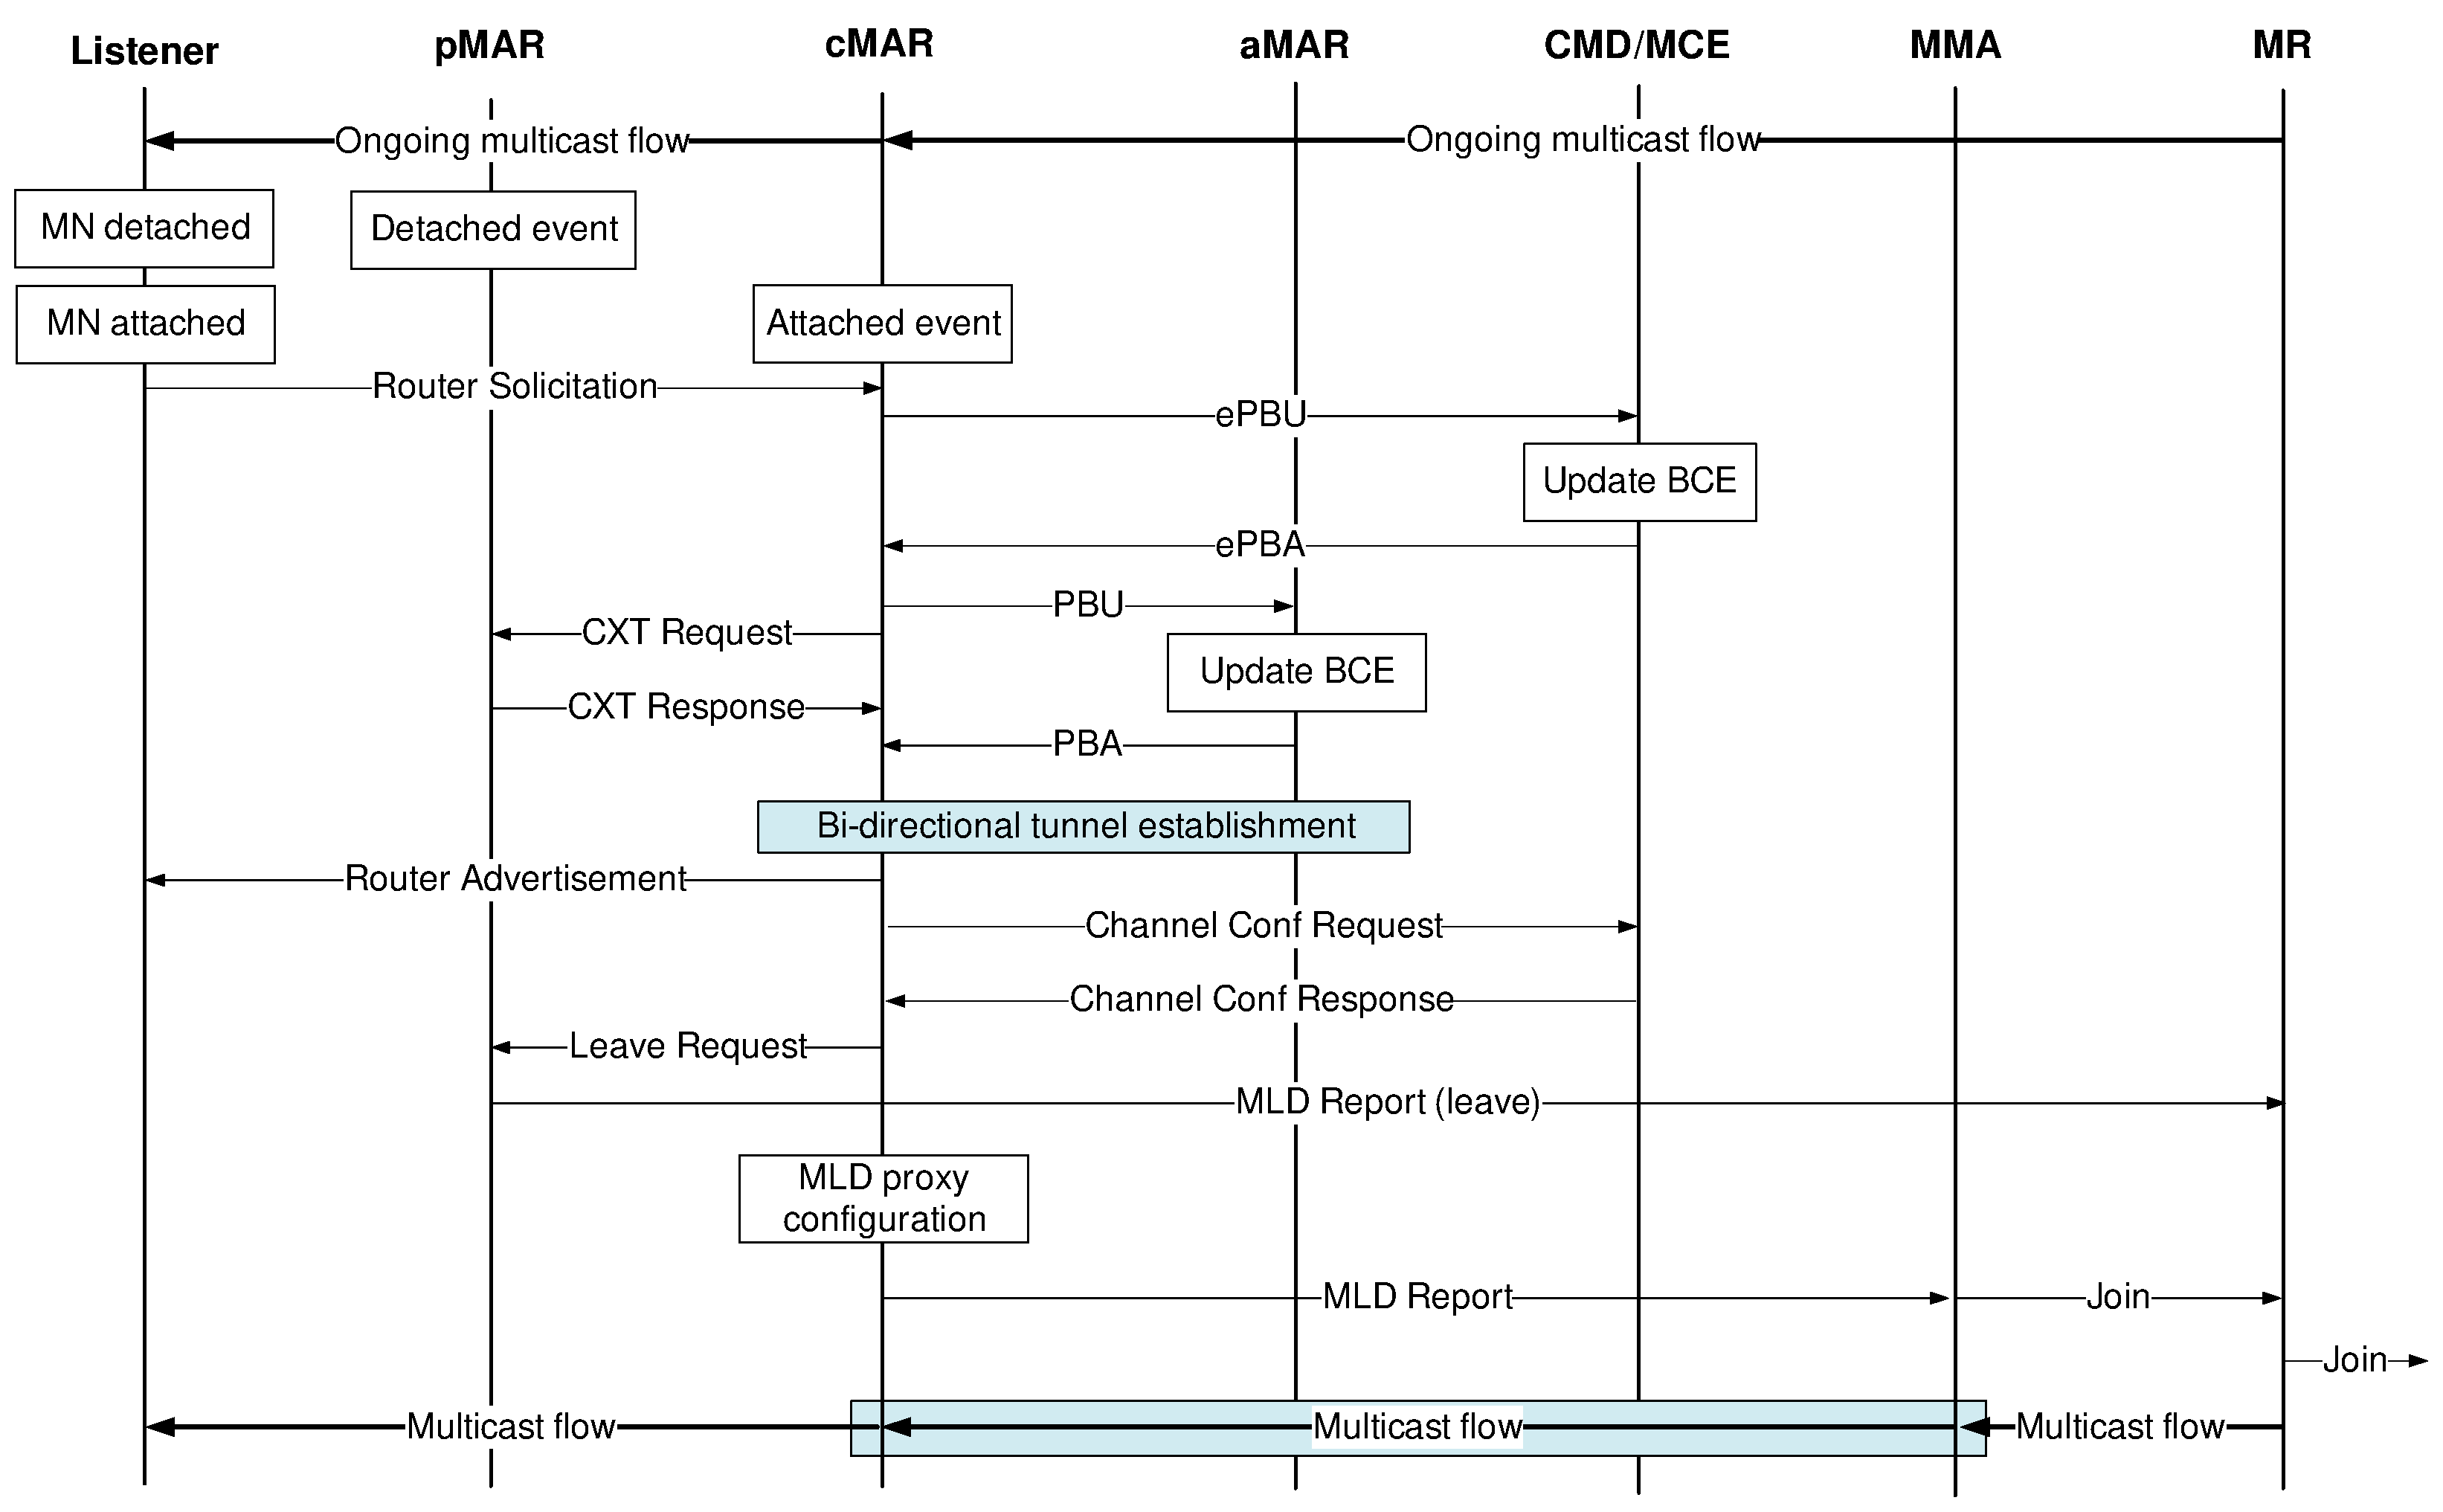
\includegraphics[width=0.85\textwidth]{./Part3/Chapter8/figures/c10_service_disruption_CXT_MMA.eps} 
    \caption{Multicast-related handover signaling with the multicast context transfer.}
    \label{fig:c10_handover_signaling}
  \end{center} 
\end{figure}

The operations of the solution are briefly introduced as follows. Once the MN enters a DMM domain (attaches to MAR1), a network prefix is allocated to it (say Pref1). MAR1 then sends a PBU message including the MN's identifier (MN\_ID) and Pref1 to the CMD to register this MN. After receiving the PBU, the CMD creates a BCE which consists of the MN\_ID, the Pref1, and the address of MAR1 (as aMAR) for this MN. In response, the PBA message is sent from CMD to MAR1 to inform that the location of the MN is updated. MAR1 then sends a Router Advertisement including the allocated prefix to the MN. The MN, after configuring its IPv6 address, can join a multicast flow via the cMAR (MAR1).

In case of handover (see Fig.~\ref{fig:c10_handover_signaling}), the cMAR allocates a new network prefix for this MN (called Pref2). The cMAR then sends a PBU to the CMD for the new prefix registration. This message includes the MN\_ID, the new prefix allocated at the current MAR (Pref2). By looking up the BCE table, the CMD updates the entry corresponding to the MN\_ID with the current location of the MN. The CMD then replies by a PBA including the list of addresses of the anchors, the corresponding prefixes, and the address of the previous MAR. Upon receiving this message, the cMAR exchanges the PBU/PBA messages with the anchor MARs to update the current location of the MN. Thus, the bi-directional tunnel is established between the cMAR and the aMAR, if necessary. The cMAR then sends a RA message including the new prefix allocated to the MN. The MN, upon this prefix, can configure its IPv6 address and start a new communication with the CN. In parallel, the multicast context transfer messages are exchanged between the cMAR and the pMAR allowing the cMAR to obtain the ongoing multicast flows of the MN. Based on this information, the cMAR contacts with the MCE to get the channel configurations which consist of the following information (per channel): S, G, MMA's address, and a field indicating the role of MMA (e.g., 0 for cMAR, 1 for pMAR, 2 for aMAR, 3 for COMMA, 4 for tMAR, and 5 for others). The PBU/PBA messages can be extended to convey the channel configuration information. The cMAR then configures an upstream interface towards the MMA, and sends an MLD report to the MMA to join the ongoing multicast channel. After joining the multicast delivery tree (if necessary), the MMA forwards the multicast packets to the cMAR, and they finally reach the MN. If the cMAR does not get the multicast traffic from the pMAR, it will request the pMAR to stop forwarding the channel. Thanks to the explicit tracking function, the pMAR stops forwarding the channel if the MN is the last member of the channel. Thus, it shortens the leave latency and reduces waste of resources. The operation in details is illustrated in Fig.~\ref{fig:c10_multicast_signaling} (Further information on the interactions between modules inside MUMO can be found in \cite{Thinh_VTC, d4.4}). 

\begin{figure}[t!]
 	\begin{center} 
		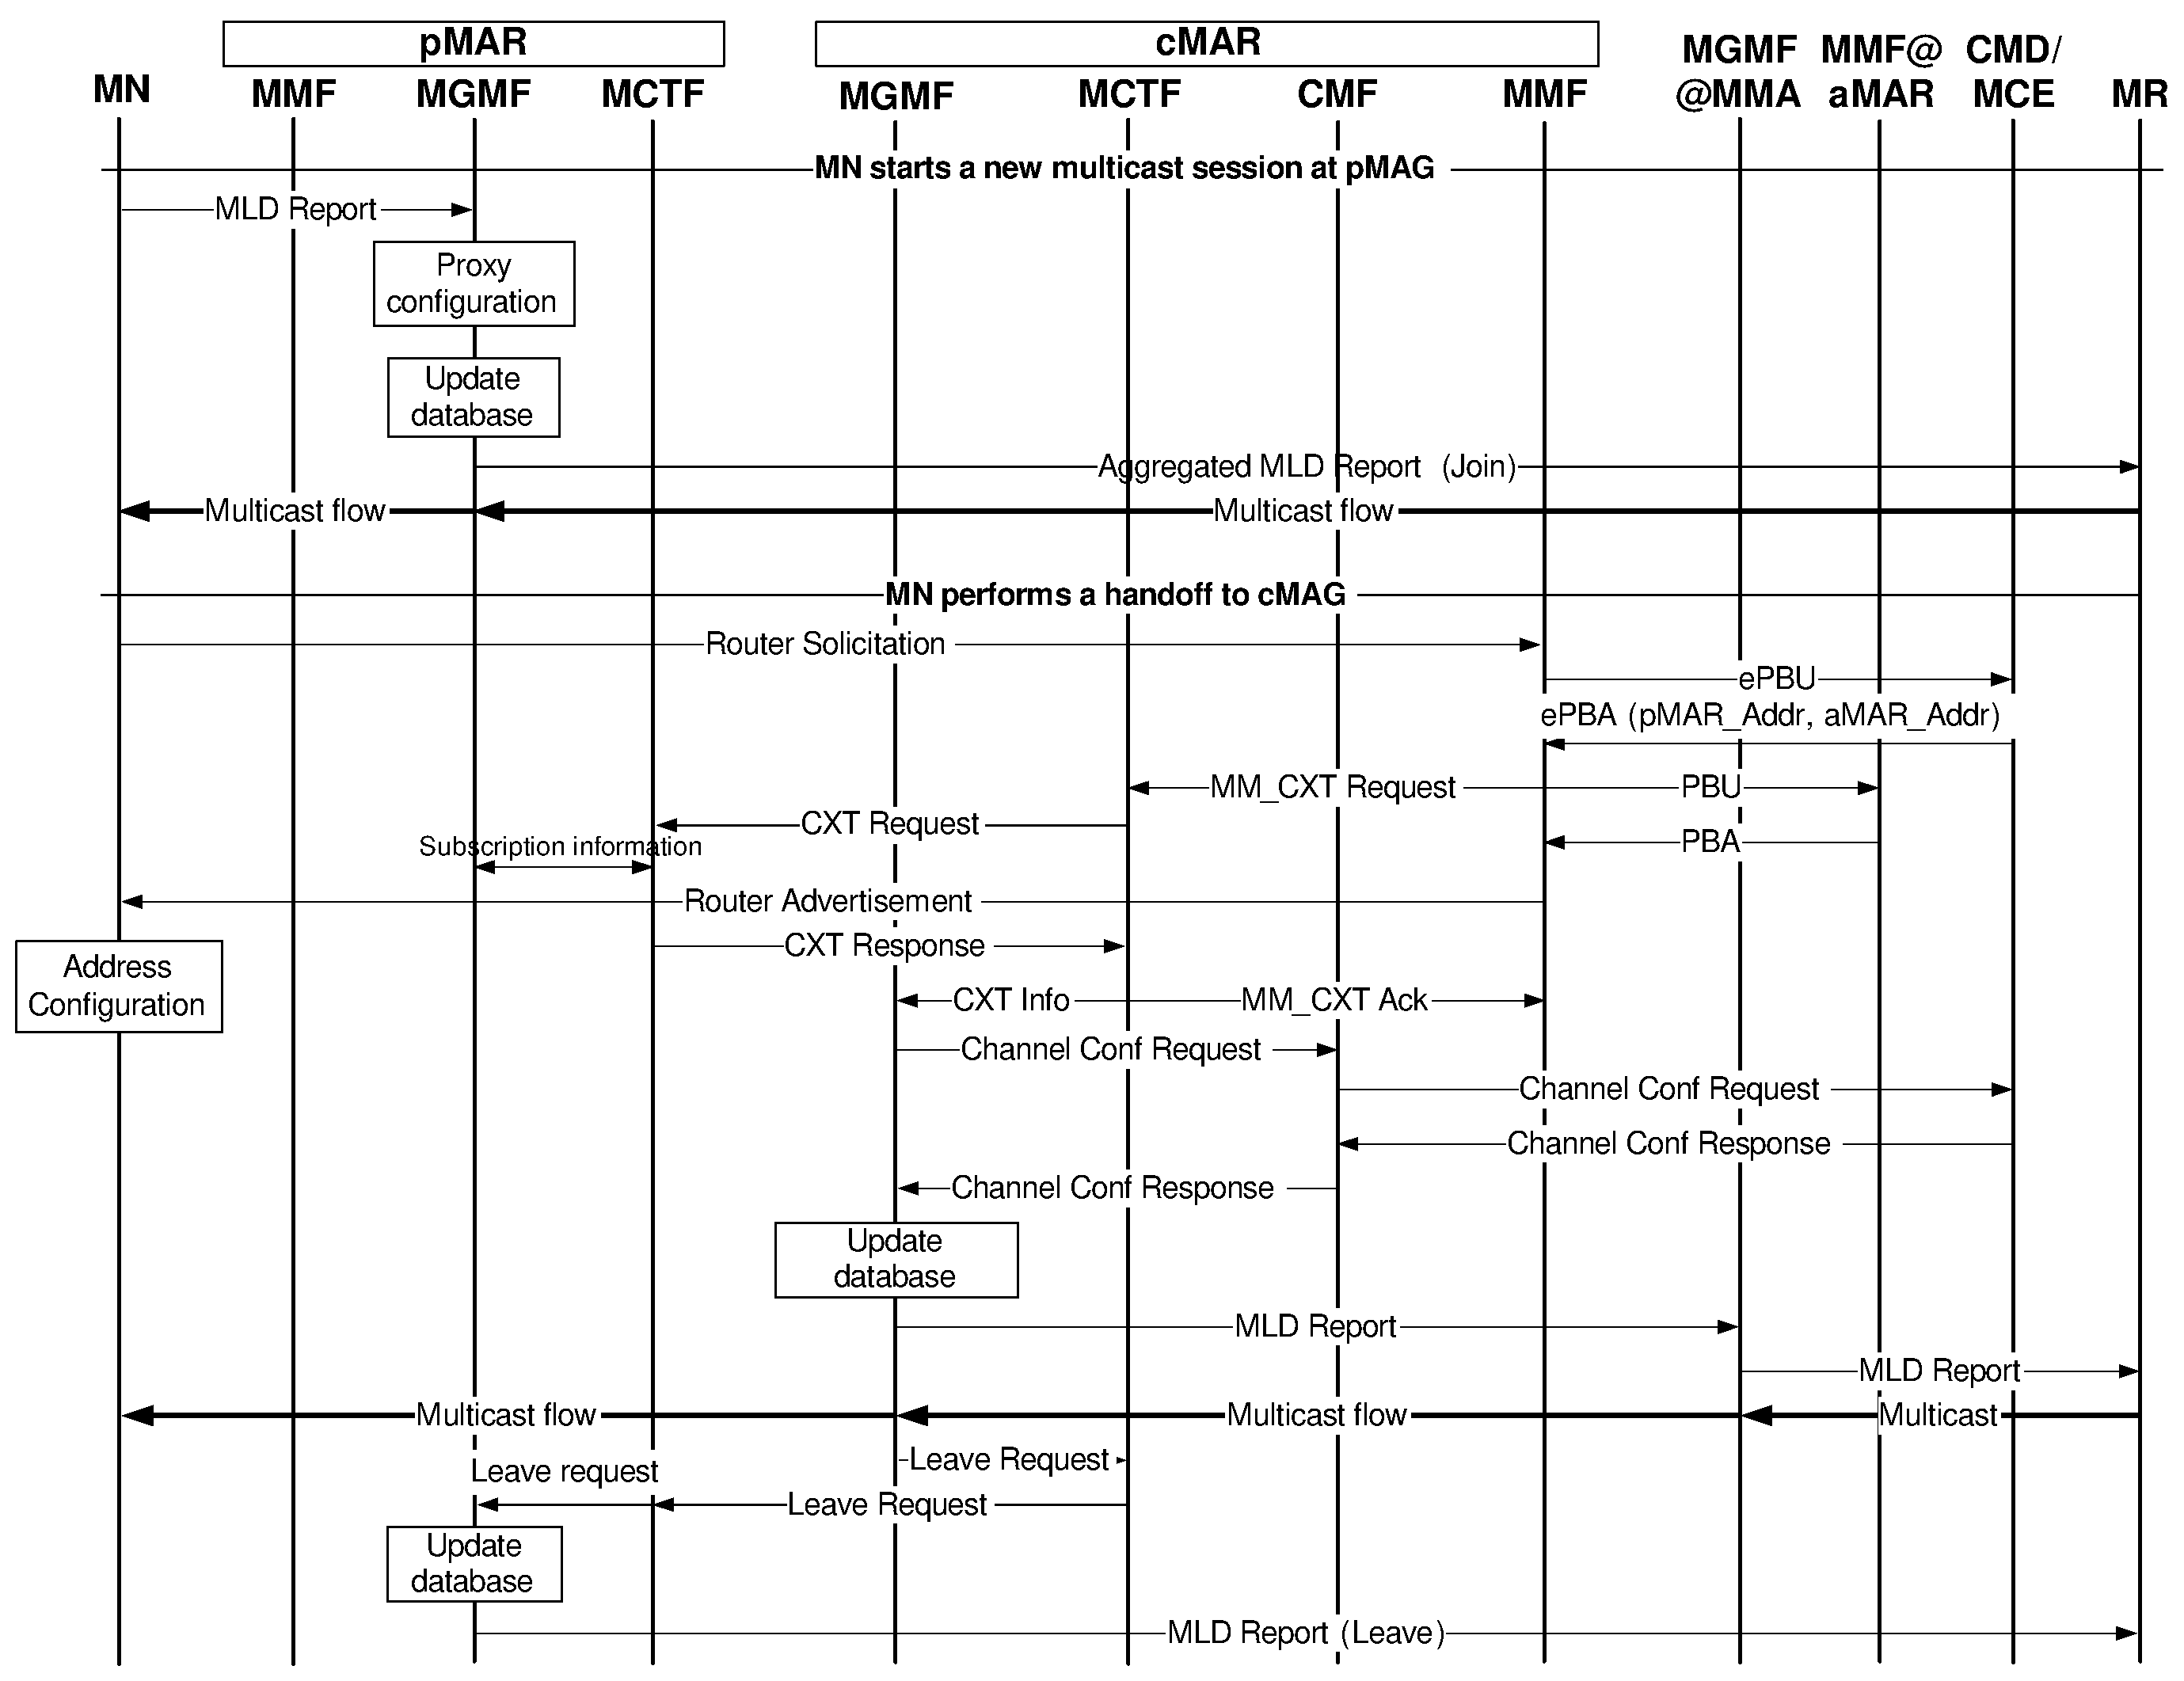
\includegraphics[width=1.05\textwidth]{./Part3/Chapter8/figures/c10_multicast_signaling.eps}
		\caption{Multicast-related handover signaling: Interactions between the modules.}
		\label{fig:c10_multicast_signaling}
	\end{center}
\end{figure}

\subsection{Other Considerations}
To reduce the complexity of MCE and the signaling cost for the context collection process, two possible enhancements can be considered as follows:
\begin{itemize}
\item The mobile node's  and the multicast service contexts can be collected and managed by the CMF module while the MCE is responsible for managing the network context\footnote{Also, in case of the fully distributed scheme, the MCE functionality will be responsible by the CMF in a distributed manner}. 
\item The MCE can store the MN's subscription information but only for the channels with strict requirement in terms of service disruption and end-to-end delay. For those channels, the MMA selection will be taken by the MCE while for the normal channels, it is done by the MUMO at the cMAR. As a result, for the channels with the strict requirement, the channel configuration will be conveyed via the extended PBA from the CMD/MCE to the cMAR. 
\end{itemize} 
\subsection{Performance Evaluation}
Compared to the performance analysis in the previous section, the DMMA may introduce an extra delay to the lowest value of the multicast service disruption (from the channel configuration acquisition process). The additional delay is calculated as \\
\begin{equation}
T_{AD} = max \lbrace T_{CXT} + T_{CF}, T_{LU} \rbrace - max \lbrace T_{CXT}, T_{LU} \rbrace,
\end{equation}
where $T_{CF}$ is the time needed for the channel configuration acquisition, and is given by\\
\begin{equation}
T_{CF} = d_{wd}(L_{CF-Req}, h_{cd}) + d_{wd}(L_{CF-Res}, h_{cd}).
\end{equation}

\begin{figure}[h!]
\centering
\subfloat[]{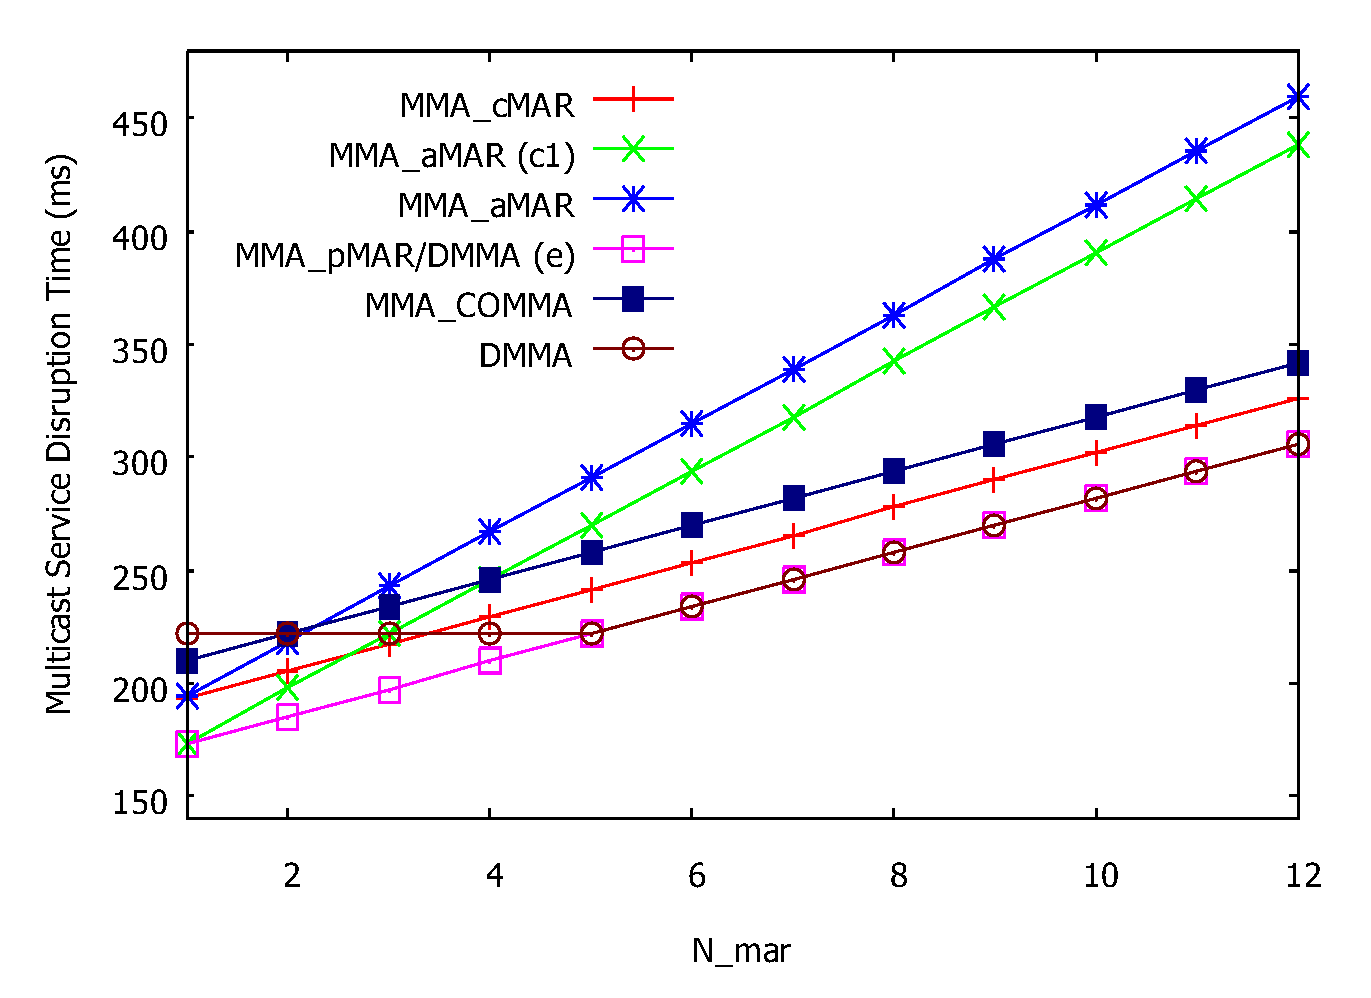
\includegraphics[width=0.50\textwidth]{./Part3/Chapter8/figures/c10_sd_ad.eps} \label{fig:c10_sd_ad}}
\subfloat[]{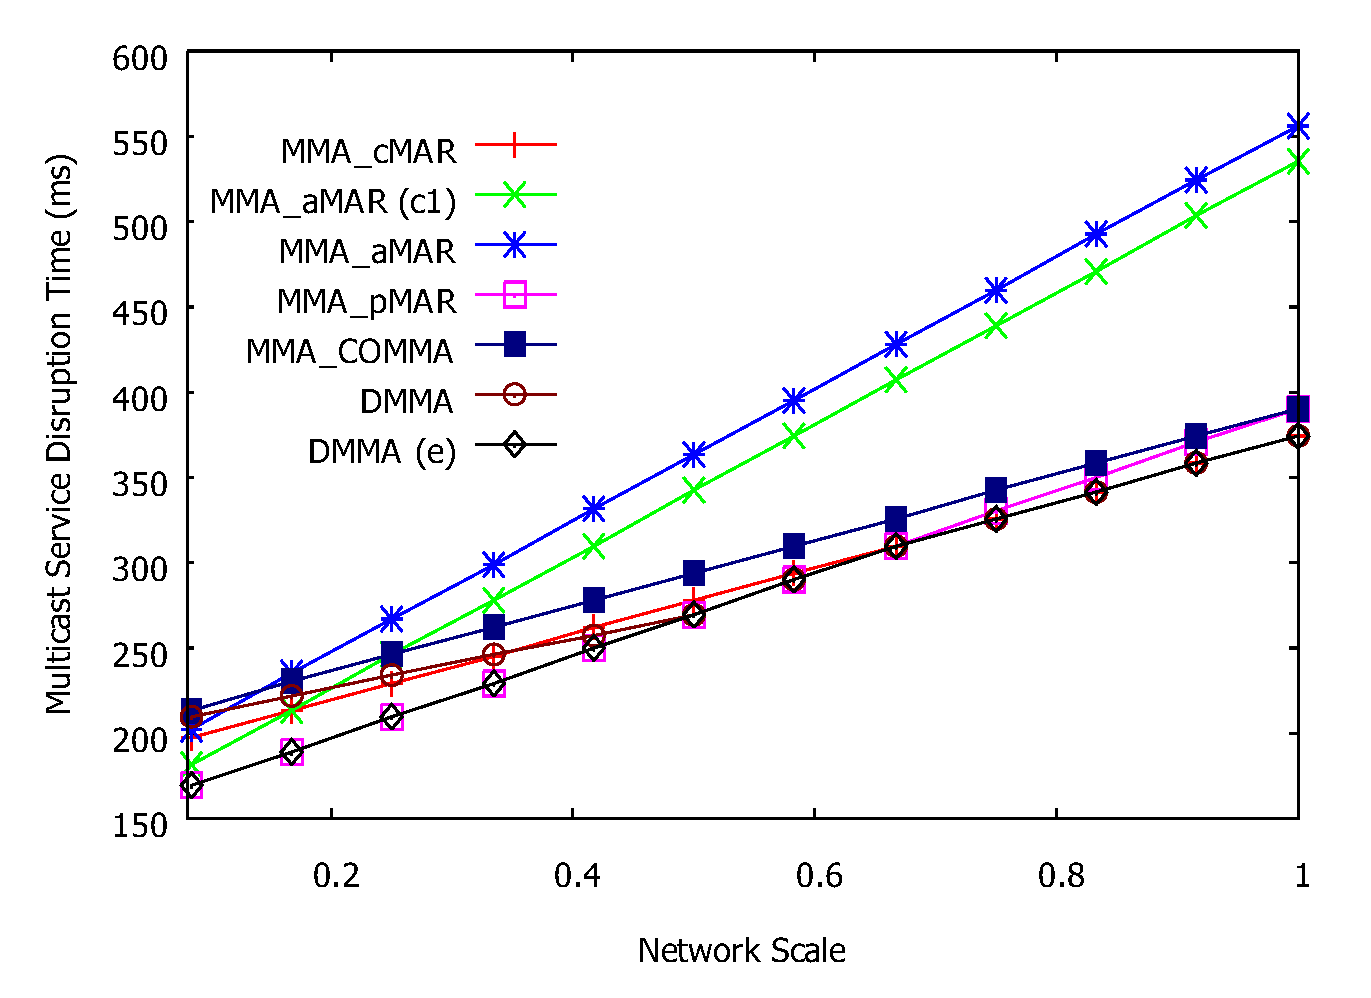
\includegraphics[width=0.50\textwidth]{./Part3/Chapter8/figures/c10_sd_ad_scale.eps}\label{fig:c10_sd_ad_scale}}\,
\subfloat[]{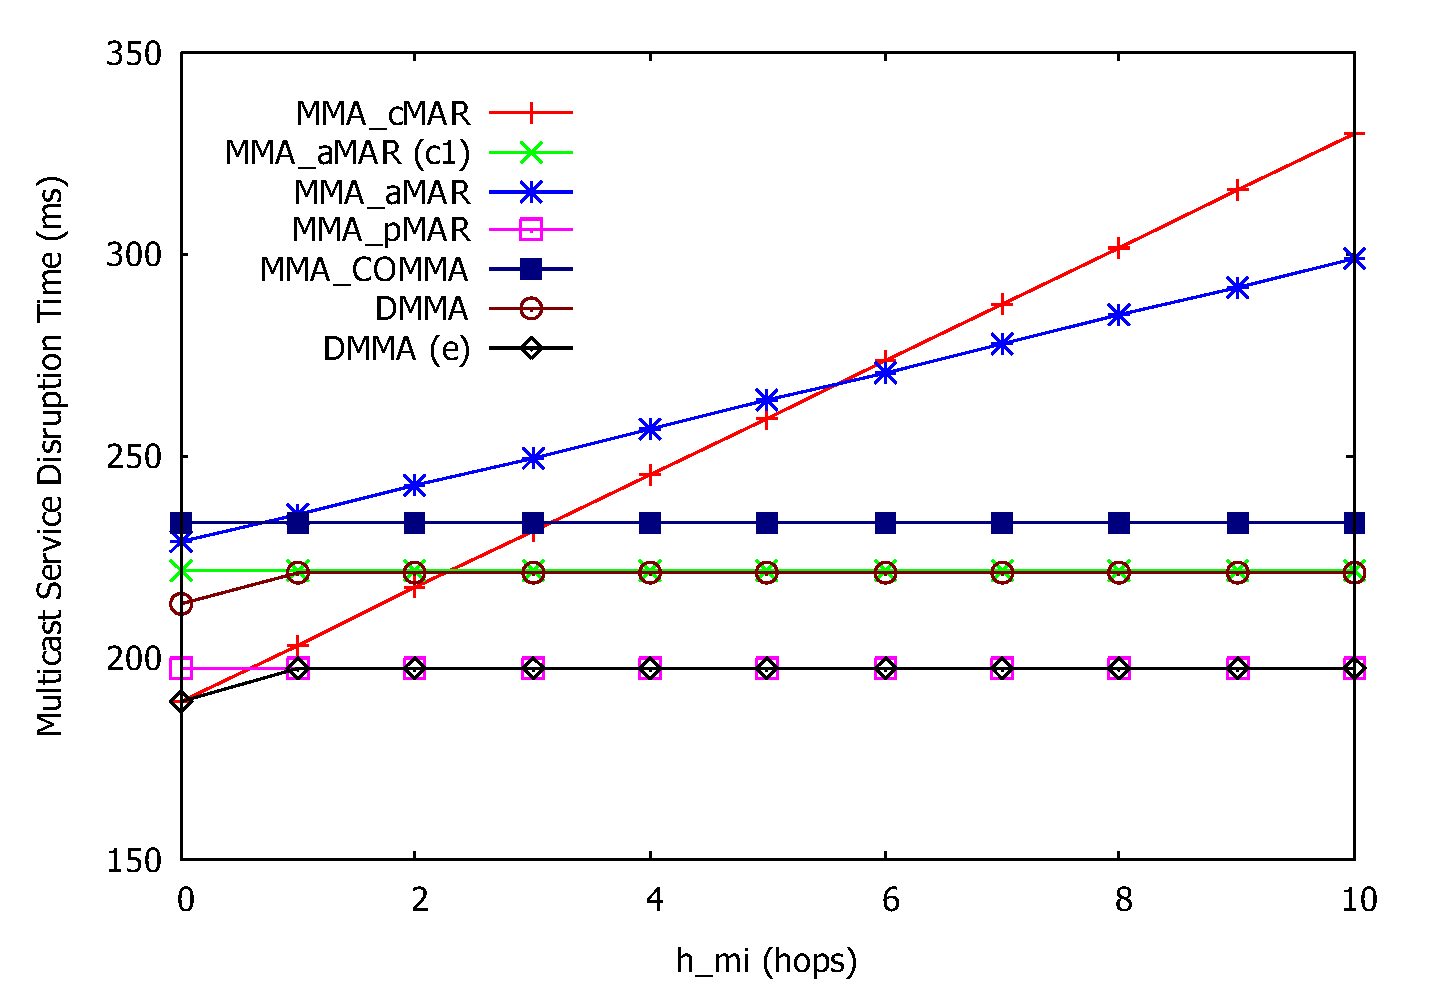
\includegraphics[width=0.50\textwidth]{./Part3/Chapter8/figures/c10_sd_ad_h_mi.eps}\label{fig:c10_sd_ad_h_mi}}
\caption[Multicast service disruption time in DMMA.]{Multicast service disruption time in DMMA: (a) $N_{mar}$, (b) $\psi$, (c) $h_{mi}$.}
\label{fig:c10_ad_all}
\end{figure}
When applying the first enhancement, the cMAR will be responsible for the MMA selection, thus, there is no need for the channel configuration acquisition. Similarly, in the second enhancement, the channel configuration information can be conveyed in the PBA message from the CMD to the cMAR. As a result, in both cases the DMMA does not introduce any additional delay. Fig.~\ref{fig:c10_sd_ad} shows the performance of the DMMA solution compared to the other approaches regarding the multicast service disruption time. 

Also, the DMMA does not introduce any extra delay regarding the end-to-end delay. The same thing happens in case of packet delivery cost, tunneling cost and packet loss. In other words, the lowest value in the end-to-end delay, packet delivery cost, tunneling cost and packet loss is set to the corresponding value of DMMA. 

\begin{figure}[h!]
\centering
\subfloat[]{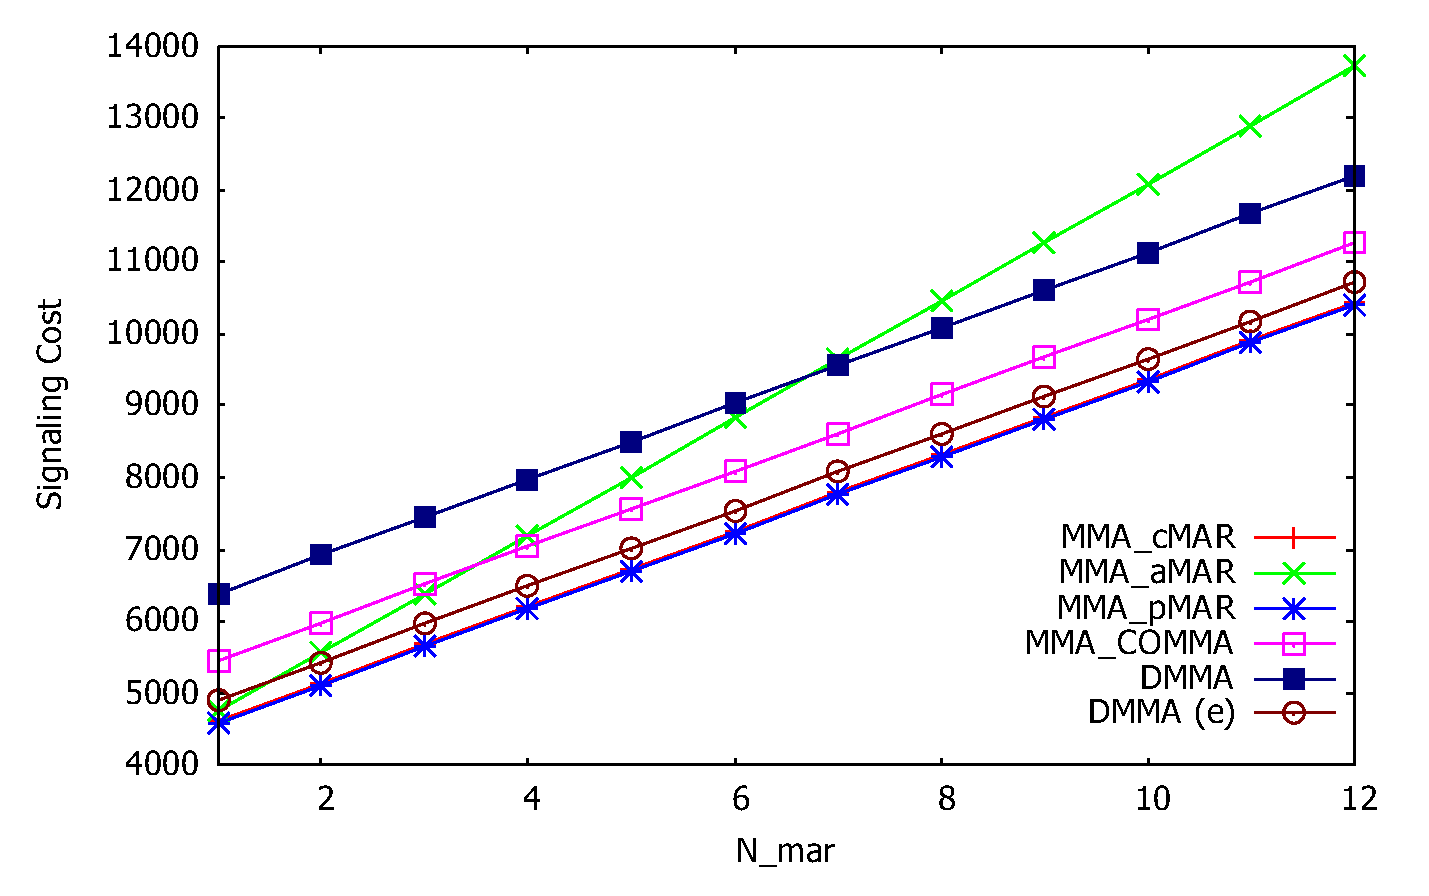
\includegraphics[width=0.50\textwidth]{./Part3/Chapter8/figures/c10_sc_ad.eps} \label{fig:c10_sc_ad}}
\subfloat[]{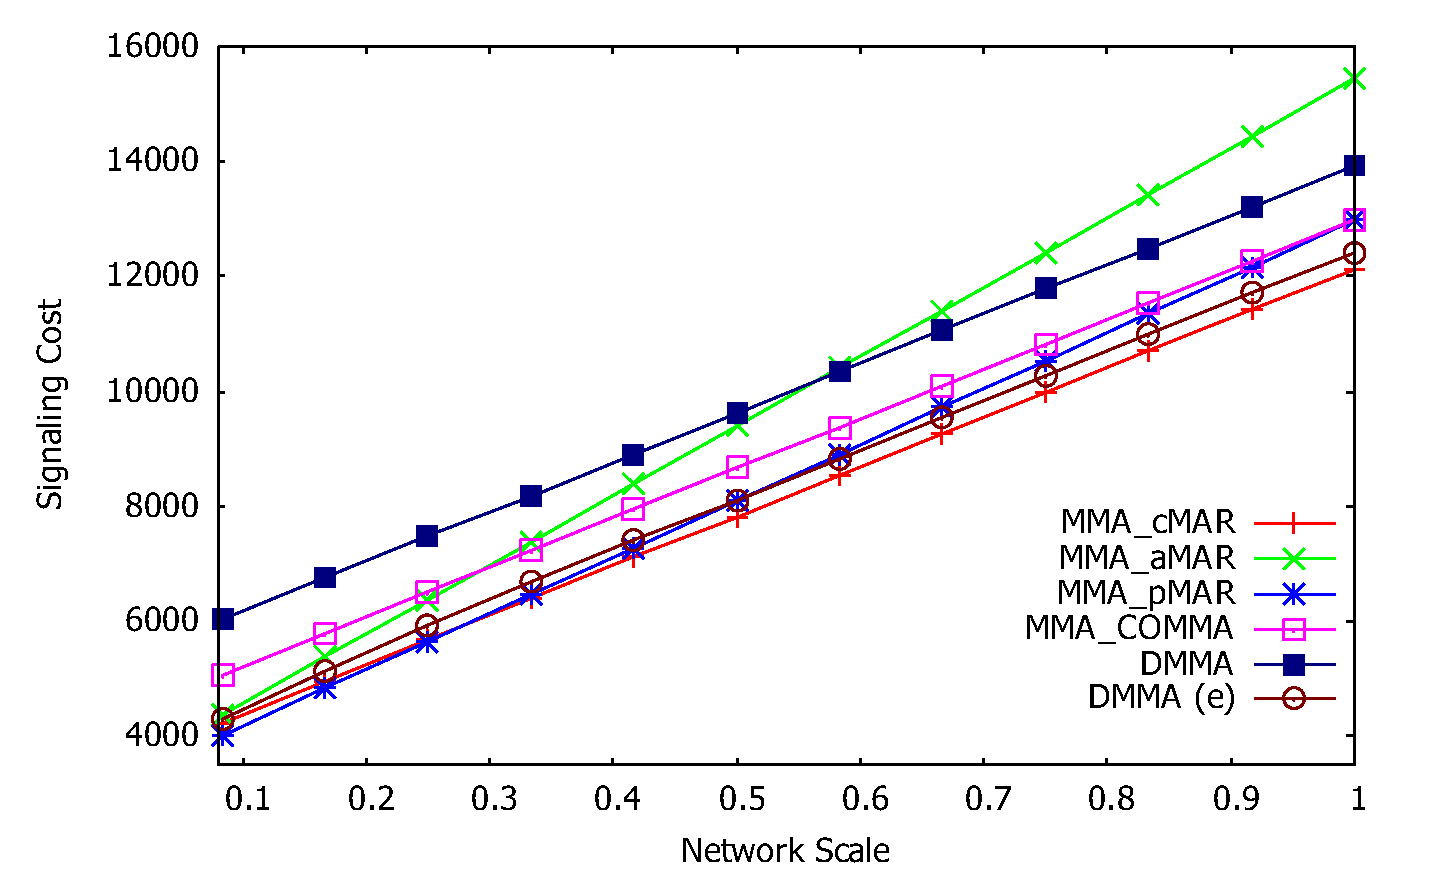
\includegraphics[width=0.50\textwidth]{./Part3/Chapter8/figures/c10_sc_ad_scale.eps}\label{fig:c10_sc_ad_scale}}\,
\subfloat[]{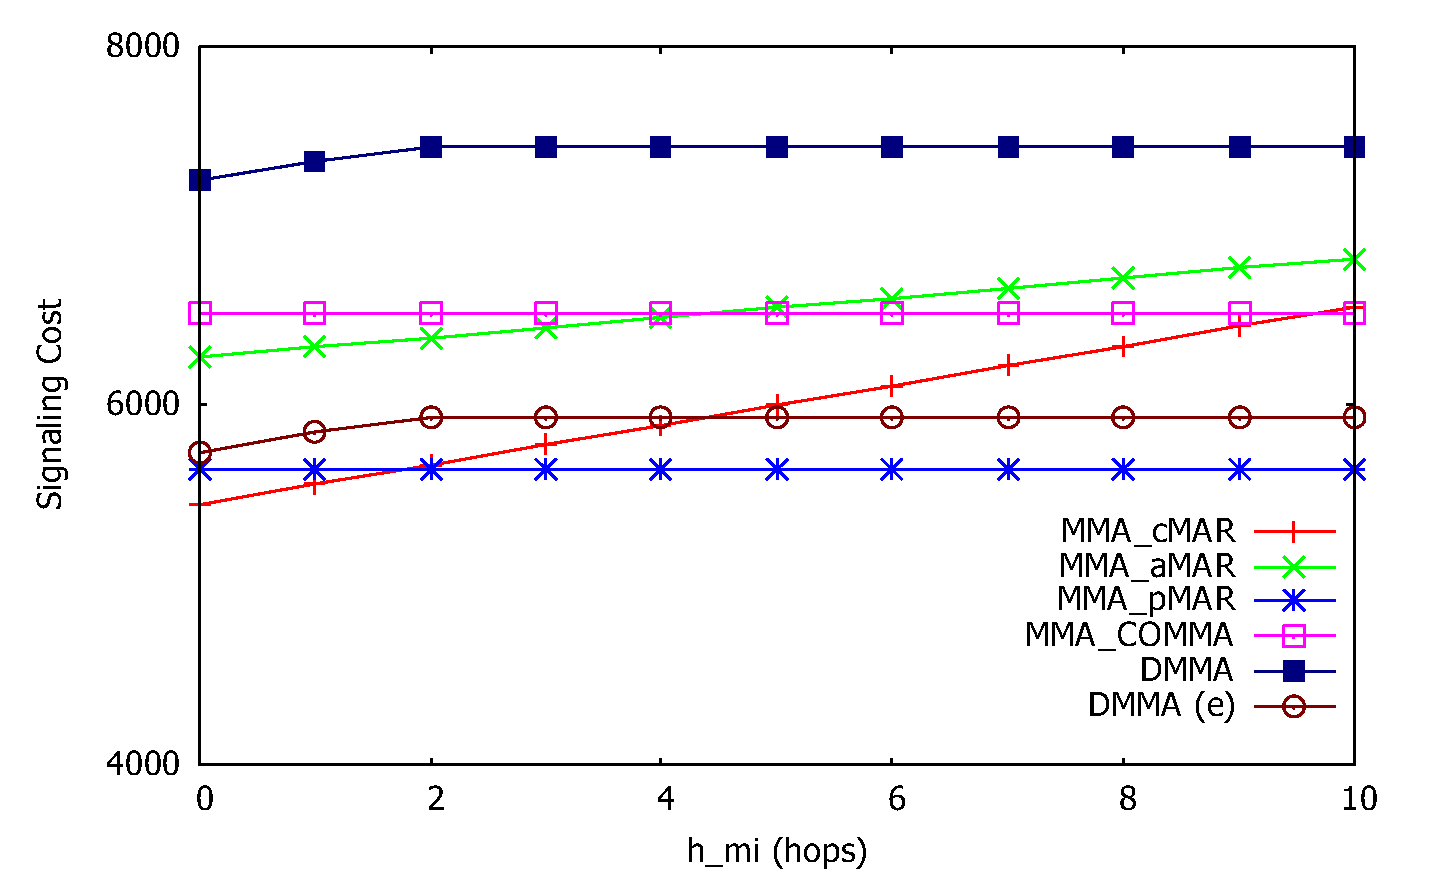
\includegraphics[width=0.50\textwidth]{./Part3/Chapter8/figures/c10_sc_ad_h_mi.eps}\label{fig:c10_sc_ad_h_mi}}
\caption[Signaling cost in DMMA.]{Signaling cost in DMMA: (a) $N_{mar}$, (b) $\psi$, (c) $h_{mi}$.}
\label{fig:c10_sc_all}
\end{figure}
Regarding the signaling cost, the additional cost is calculated as\\
\begin{equation}
SC_{AD} =\alpha L_{CF-Req} h_{cd} + \alpha L_{CF-Res} h_{cd} + \alpha L_{leave} h_{pc},
\end{equation}
where $L_{leave}$ is the size of the leave request message sent from the cMAR to the pMAR, which is 96 bytes. When applying these enhancements, the additional cost is only derived from the leave request message. Fig.~\ref{fig:c10_sc_all} shows the performance of the DMMA solution compared to the other approaches regarding the signaling cost. The signaling cost in case of DMMA is quite high compared to that in the MMA\_pMAR and MMA\_cMAR. On the contrary, in case of DMMA (e) it is slightly higher than the lowest value as an acceptable cost for the reduction of other metrics (service disruption time, end-to-end delay, packet delivery cost, tunneling cost). 

\section{Discussions}\label{c10:discussion}
\subsection{Implementation Work}
An early version of the DMMA was available thanks to the Medieval project \cite{d4.4, d6.4, ICC_Sergio}. In this implementation, the context management module (CMF) executes in a simple way: when the MN acts as a multicast listener, the cMAR always plays the role of the MMA. On the contrary, the aMARs acts as the MMA when the MN plays the role of a multicast source. 
However, the procedures for the considered contexts acquisition are still under development. Aslo, the MMF module is being developed based on the OAI PMIPv6 implementation. The other modules i.e., MGMF and MCTF are already available as described in Chapter \ref{ch:performance_evaluation} and Chapter \ref{ch:multicast_PMIP}. In the next step, the full implementation of the CMF module will be deployed. Experiments then will be conducted based on the testbed using the method described in Chapter \ref{ch:performance_evaluation}. 


\subsection{Multicast Router Function Deployment at MAR}
Our analysis can also be applied when the multicast router function is deployed at MAR. As in the Medieval project, the MGMF represents the functionality of a multicast router (e.g., based on MRD6 implementation). In this case, the Multicast Routing Information Base (MRIB) can be not only based on the unicast RIB, but also on the information from the CMF. For example, in order to set the pMAR as the upstream multicast router for a specific channel (say C1), the cMAR uses an explicit PIM join message to join the C1 at pMAR. In other words, pMAR becomes a RPF neighbor router of the cMAR regarding the channel C1. 

\subsection{Multicast Source Mobility Support}
At this stage, our solution can also support source mobility in DMM. However, the aMAR will always act as the MMA for the source to avoid the potential impact on the service disruption. In case of ASM, an extension of PIM-SM \cite{explicit_rpf} can be used to route the multicast traffic directly from the cMAR to the RP bypassing the aMAR. Thus, the multicast traffic is routed in a better way. In more details, the explicit reserve path forwarding (RPF) mechanism is used to build the multicast delivery tree via an explicitly configured path included in the PIM join messages. After receiving the unicast-encapsulation packets from the current MAR, the RP will send a Join message including the address of the sender (cMAR's address) in a new type-length-vector (TLV). It allows the RP to establish the shortest path tree towards the current location of the source. The native multicast traffic then will be sent via the new delivery tree from the cMAR and reaches the listeners (PIM phase two).  

\section{Conclusion}\label{c10:conclusion}
In this chapter, we have presented a performance analysis for different approaches to support the multicast listener mobility in DMM. The analytical results can be very useful in the design of IP mobile multicast solutions in a DMM environment. We argued that, under certain scenarios, it is hardly possible to achieve the requirements in terms of service interruption and delay for specific services (e.g., real-time service). We then introduced a dynamic multicast mobility anchor mechanism in order to mitigate these issues. This mechanism takes into account various contexts ranging from the multicast service, the mobile node's mobility to the network context, thereby, enabling a per-flow multicast support. Numerical results showed that for each scenario these requirements can be satisfied. Also, several benefits can be offered such as tunnel convergence avoidance, effective tunnel management, route optimization and waste of resource reduction. 
